\documentclass{article}
\usepackage[final]{graphicx}
\graphicspath{{graphes/}}
\usepackage{amsmath}
\usepackage{amssymb} % AJOUT (correctif de compilation) : requis pour \mathbb et \lesssim
\usepackage{float}
\usepackage{booktabs}
\usepackage[utf8]{inputenc}
\usepackage[T1]{fontenc}
\usepackage[english]{babel}
\usepackage{indentfirst}
\usepackage{graphicx}
\usepackage{xcolor} % AJOUT : couleur pour les corrections
\usepackage[colorlinks=true,
            linkcolor=blue,
            urlcolor=blue,
            citecolor=blue]{hyperref}
\usepackage{geometry}
\usepackage{ragged2e}
\usepackage{xurl}
\usepackage{enumitem}
\geometry{margin=2.5cm}
\date{}
\justifying
\newcommand{\rev}[1]{{\color{red}#1}}
\providecommand{\og}{«~}
\providecommand{\fg}{~»}
\providecommand{\up}[1]{\textsuperscript{#1}}
\title{Summer Project : Du modèle à la stratégie : un cadre jump-diffusion pour le pairs trading}
\begin{document}
\maketitle
\section{Le pairs trading}
\subsection{Principe général}
Le pairs trading est né au début des années 1980 chez Morgan Stanley. Le concept est en lui-même assez simple, mais lorsque nous y regardons de plus près, celui-ci est en fait plutôt complexe. L'idée principale est la suivante. Prenons deux actifs qui sont en quelque sorte "liés" l'un à l'autre comme Coca-Cola et PepsiCo : deux entreprises cotées, directement concurrentes, qui vendent des produits similaires et subissent les mêmes chocs (coûts des alimentaires, salaires, réglementation, humeur des consommateurs). Leurs cours de bourse ont donc tendance à bouger ensemble sur le long terme. Mais de temps en temps, l'un des deux prend temporairement de l'avance sur l'autre --- une nouvelle, un flux d'acheteurs, rien de fondamental. Le pari du pairs trading est simple : cet écart va se résorber. On achète celui qui est temporairement « trop bas », on vend (à découvert) celui qui est « trop haut », et on gagne quand ils se rapprochent, que le marché entier monte ou descende, cela ne change, en première approximation, rien. C'est ce qu'on appelle une stratégie market-neutral.\\
\subsubsection{Market neutral}
C'est une stratégie d'investissement conçue pour rendre le rendement, en première approximation, insensible à l'exposition linéaire au facteur marché. Cette neutralité est conditionnelle à la stabilité des bêtas estimés et ne protège pas des expositions non linéaires (convexités, corrélations qui augmentent en période de crise) : elle ne rend pas le rendement \emph{indépendant} du marché au sens probabiliste. Il y a plusieurs niveaux de neutralité :
\begin{enumerate}
    \item \textbf{Neutralité en dollars} : Valeur longue = Valeur courte.
    \item \textbf{Neutralité en beta (beta-neutral)} : $\sum_i w_i \beta_i = 0$, on pondère les positions de façon à ce que la somme des betas (sensibilité au marché) s'annule.
    \item \textbf{Neutralité sectorielle/factorielle} : On neutralise aussi l'exposition à des facteurs comme la taille (size), la value, le momentum, etc., pour isoler un pur signal de sélection.
\end{enumerate}
\subsubsection{Explication de $\beta$ et $w_i$}
Dans la formule
\begin{equation}
    \sum_i w_i \beta_i = 0,
\end{equation}
$w_i$ et $\beta_i$ sont deux éléments clés de la construction de portefeuille.
\paragraph{$w_i$ : le poids de l'actif $i$.}
C'est la pondération (ou taille relative) de la position sur l'actif $i$ dans le portefeuille :
\begin{equation}
    w_i = \frac{\text{Valeur de la position sur l'actif } i}{\text{Valeur totale du portefeuille}}.
\end{equation}
\begin{itemize}
    \item $w_i > 0$ $\rightarrow$ position \textbf{longue} (achat)
    \item $w_i < 0$ $\rightarrow$ position \textbf{courte} (vente à découvert)
    \item $|w_i|$ $\rightarrow$ l'ampleur de la position
\end{itemize}
\paragraph{Exemple.} Portefeuille de 100~000\$ avec :
\begin{itemize}
    \item 60~000\$ investis en position longue sur Apple $\rightarrow$ $w_{\text{Apple}} = +0{,}6$
    \item 40~000\$ en position courte sur Microsoft $\rightarrow$ $w_{\text{Microsoft}} = -0{,}4$
\end{itemize}
\paragraph{$\beta_i$ : le beta de l'actif $i$.}
Le beta mesure la sensibilité du rendement de l'actif $i$ par rapport au rendement du marché (souvent représenté par un indice comme le S\&P~500). Il est estimé par régression linéaire :
\begin{equation}
    R_i = \alpha_i + \beta_i R_m + \varepsilon_i,
\end{equation}
où :
\begin{itemize}
    \item $R_i$ : rendement de l'actif $i$
    \item $R_m$ : rendement du marché
    \item $\alpha_i$ : rendement ``anormal'' (indépendant du marché), souvent la grandeur que l'on cherche à capturer
    \item $\varepsilon_i$ : terme d'erreur
\end{itemize}
Mathématiquement, $\beta_i$ correspond à :
\begin{equation}
    \beta_i = \frac{\text{Cov}(R_i, R_m)}{\text{Var}(R_m)}.
\end{equation}
On notera que $\beta_i = \rho_{im}\,\sigma_i/\sigma_m$ : le bêta mesure la sensibilité \emph{systématique} de l'actif au marché, et non sa volatilité totale. Un actif de faible bêta peut être très volatil si son risque idiosyncratique est important.
\begin{table}[H]
    \centering
    \begin{tabular}{ll}
        \toprule
        \textbf{Valeur de $\beta$} & \textbf{Signification} \\
        \midrule
        $\beta = 1$      & L'actif bouge en moyenne comme le marché \\
        $\beta = 2$      & En moyenne, l'actif varie de 2\,\% quand le marché varie de 1\,\% (composante systématique) \\
        $\beta = 0{,}5$  & En moyenne, l'actif varie de 0{,}5\,\% quand le marché varie de 1\,\% ; sa volatilité totale peut néanmoins excéder celle du marché \\
        $\beta = 0$      & L'actif est non corrélé (linéairement) avec le marché \\
        $\beta < 0$      & L'actif évolue en moyenne en sens inverse du marché \\
        \bottomrule
    \end{tabular}
    \caption{Interprétation du coefficient $\beta$}
    \label{tab:beta_interpretation}
\end{table}
La question est maintenant la suivante : comment rendre rigoureux, mathématiquement, l'idée que "ces deux prix sont liés" et que "leur écart va se résorber" ? Toute tentative de réponse se heurte d'abord à un obstacle : un prix, pris seul, n'a pas de moyenne vers laquelle revenir.
\subsection{Pourquoi on ne peut pas prédire un prix seul ?}
Un modèle de référence, difficile à battre empiriquement en prévision,  pour décrire l'évolution d'un prix financier est la \textbf{marche aléatoire} :
\begin{equation}
P_{t+1} = P_t + \varepsilon_{t+1}
\label{eq:rw}
\end{equation}
où $\varepsilon_{t+1}$ est un bruit aléatoire d'espérance nulle, imprévisible à partir de l'information disponible en $t$. Trois précisions de cadrage s'imposent. Premièrement, la convention d'indexation : l'innovation qui réalise le passage de $t$ à $t+1$ est notée $\varepsilon_{t+1}$, car elle est $\mathcal{F}_{t+1}$-mesurable et non $\mathcal{F}_t$-mesurable. En effet, $\varepsilon_{t+1}=P_{t+1}-P_t$ est mesurable par rapport à $\mathcal{F}_{t+1}=\sigma(P_0,\dots,P_{t+1})$ : c'est une fonction (la différence) de deux quantités déjà contenues dans cette tribu, donc elle en hérite la mesurabilité. Elle ne peut en revanche être $\mathcal{F}_t$-mesurable : si elle l'était, elle serait connue dès l'instant $t$ et sortirait de l'espérance conditionnelle comme une constante, $E[\varepsilon_{t+1}\mid\mathcal{F}_t]=\varepsilon_{t+1}$ ; combinée à l'hypothèse $E[\varepsilon_{t+1}\mid\mathcal{F}_t]=0$ du modèle, cela imposerait $\varepsilon_{t+1}=0$ presque sûrement, c'est-à-dire un bruit nul et un prix parfaitement prévisible, exactement ce que le modèle de marche aléatoire exclut par construction.
Deuxièmement, cette spécification omet toute dérive : les prix d'actions présentent empiriquement un drift positif de long terme, et la formulation complète serait $P_{t+1}=\mu+P_t+\varepsilon_{t+1}$ ; nous posons $\mu=0$ pour simplifier l'exposition. Troisièmement, une marche aléatoire additive autorise des prix négatifs ; la convention standard applique ce modèle au log-prix $\ln P_t$, convention que nous adoptons implicitement dans tout ce travail (cf. sous-partie 2.4). Cette équation énonce un résultat en apparence décourageant : la meilleure prévision du prix de demain, $E[P_{t+1} \mid P_t]$, est simplement le prix d'aujourd'hui, $P_t$. Il n'existe, à partir du passé du prix, aucune information permettant d'anticiper en espérance s'il va monter ou descendre. Cette propriété porte un nom : un processus intégrable et adapté dont l'espérance conditionnelle future est égale à sa valeur présente est appelé une \textbf{martingale}. Montrons ce résultat explicitement. En prenant l'espérance conditionnelle de l'équation~\eqref{eq:rw}, sachant l'information disponible en $t$ ($P_0$, $P_1$, ...,$P_t$, notée $\mathcal{F}_t$, qui contient en particulier $P_t$) :
\begin{align}
E[P_{t+1} \mid \mathcal{F}_t] &= E[P_t + \varepsilon_{t+1} \mid \mathcal{F}_t] \\
&= E[P_t \mid \mathcal{F}_t] + E[\varepsilon_{t+1} \mid \mathcal{F}_t] \\
&= P_t + E[\varepsilon_{t+1} \mid \mathcal{F}_t]
\end{align}
La première égalité découle de la linéarité de l'espérance. La seconde utilise le fait que $P_t$ est déjà connu à l'instant $t$ (il est donc une constante conditionnellement à $\mathcal{F}_t$, et sort de l'espérance sans modification). Il reste à évaluer le second terme : par construction, $\varepsilon_{t+1}$ représente un bruit imprévisible à partir de l'information passée et est d'espérance nulle, c'est-à-dire
\begin{equation}
E[\varepsilon_{t+1} \mid \mathcal{F}_t] = 0.
\end{equation}
En substituant, on obtient :
\begin{equation}
E[P_{t+1} \mid \mathcal{F}_t] = P_t.
\end{equation}
C'est précisément la définition d'une \textbf{martingale} (sous réserve d'intégrabilité, $E[|P_t|]<\infty$, et d'adaptation à la filtration $(\mathcal{F}_t)$, deux conditions vérifiées ici) : l'espérance conditionnelle de la valeur future, sachant tout ce qui s'est passé jusqu'à présent, est égale à la valeur actuelle. Par la loi des espérances itérées, la propriété à un pas s'étend à tout horizon : $E[P_{t+s}\mid\mathcal{F}_t]=P_t$ pour tout $s\geq 0$. Aucune information contenue dans l'historique du prix ne permet donc d'anticiper en espérance un mouvement à la hausse ou à la baisse. 
Cette absence de prévisibilité a une conséquence directe sur la variance du processus. En itérant la relation depuis un instant initial $0$ :
\begin{equation}
P_t = P_0 + \sum_{i=1}^{t} \varepsilon_i
\end{equation}\\
En supposant de plus l'homoscédasticité, $\text{Var}(\varepsilon_i)=\sigma_\varepsilon^2$ pour tout $i$, hypothèse supplémentaire, qui ne découle pas de la seule propriété de martingale, et en notant que $E[\varepsilon_j\mid\mathcal{F}_{j-1}]=0$ avec $\varepsilon_i\in\mathcal{F}_{j-1}$ pour $i<j$ implique $\text{Cov}(\varepsilon_i,\varepsilon_j)=0$ :  \\
\begin{align}
\text{Var}(P_t \mid P_0)&= \text{Var}\left(\sum_{i=1}^{t} \varepsilon_i\right)
&& \text{($P_0$ constante, n'affecte pas la variance)} \\
&= \sum_{i=1}^{t} \text{Var}(\varepsilon_i) + 2\sum_{i<j} \text{Cov}(\varepsilon_i, \varepsilon_j)
&& \text{(variance d'une somme)} \\
&= \sum_{i=1}^{t} \text{Var}(\varepsilon_i)
&& \text{(non-corrélation, établie ci-dessus}) \\
&= t \, \sigma_\varepsilon^2
&& \text{(} \text{Var}(\varepsilon_i) = \sigma_\varepsilon^2 \text{)}
\end{align}
La variance du prix croît linéairement avec le temps, sans jamais se stabiliser. Autrement dit, plus on regarde loin dans le futur, plus l'incertitude sur la position du prix est grande, il n'existe aucune borne vers laquelle cette incertitude convergerait.
Cette propriété distingue la marche aléatoire d'un processus \textbf{stationnaire} au second ordre, c'est-à-dire un processus dont la moyenne, la variance et la structure de covariance temporelle restent constantes dans le temps. Précisons que la stationnarité garantit l'existence d'un niveau moyen fixe, mais pas, à elle seule, un \og retour \fg{} rapide vers ce niveau : la \emph{vitesse} de retour à la moyenne, déterminante pour le trading, est une propriété supplémentaire, quantifiée en sous-partie 2.6. Un prix financier, suivant une marche aléatoire, ne possède aucune de ces propriétés : il n'a pas de niveau d'équilibre, et donc pas de « moyenne » vers laquelle revenir. Parier sur un retour à la moyenne d'un prix pris isolément n'a, dans ce cadre, c'est-à-dire conditionnellement au modèle de marche aléatoire, aucun fondement statistique.
Ce constat est le mur conceptuel que le pairs trading doit contourner : puisqu'un prix seul n'offre aucune prise au retour à la moyenne, il s'agit de construire, à partir de deux prix non-stationnaires, une nouvelle quantité qui, elle, le soit. C'est précisément l'objet de la notion de cointégration, introduite dans la sous-partie suivante.
\subsection{Corrélation ou cointégration ?}
La sous-partie précédente a établi qu'un prix pris isolément ne revient jamais vers une valeur d'équilibre. La question devient alors : peut-on trouver, à partir de \emph{deux} prix non-stationnaires, une manière de capturer un lien suffisamment fort entre eux pour fonder une stratégie de retour à la moyenne ? La réponse intuitive\rev{,} utiliser la corrélation\rev{,} s'avère insuffisante, pour une raison qu'il convient de détailler avant d'introduire le bon outil : la cointégration.
\subsubsection*{Ce que mesure (et ne mesure pas) la corrélation}
La corrélation entre deux variables aléatoires de variance finie $X$ et $Y$ se définit par :
\begin{equation}
\rho(X,Y) = \frac{\text{Cov}(X,Y)}{\sigma_X \, \sigma_Y}
\end{equation}
Cette quantité, comprise entre $-1$ et $1$, mesure l'intensité d'une association \emph{linéaire et contemporaine} : si $X$ augmente, $Y$ a-t-il tendance à augmenter également, au même instant ? En finance, la corrélation est le plus souvent calculée sur les \emph{rendements} (variations relatives de prix), non sur les prix eux-mêmes.
Cette mesure ne dit cependant rien sur ce qui se passe à long terme. Deux prix peuvent avoir des rendements fortement corrélés, ils montent et descendent ensemble, jour après jour -- tout en s'éloignant progressivement et indéfiniment l'un de l'autre en niveau. La corrélation des rendements est une propriété \emph{instantanée} : elle ne garantit aucune relation d'équilibre stable dans le temps, et donc aucune raison statistique de parier sur un rapprochement futur des deux prix.
\subsubsection*{Une image pour distinguer les deux notions}
L'illustration classique de cette distinction est la suivante. Considérons deux ivrognes qui marchent chacun au hasard dans une rue, indépendamment l'un de l'autre : chacun suit une marche aléatoire. Rien n'empêche la distance qui les sépare de croître sans limite au fil du temps, cette distance est elle-même une marche aléatoire, sans niveau d'équilibre.
Considérons à présent une femme ivre promenant son chien en laisse. Elle marche au hasard ; son chien aussi, tirant tantôt à gauche, tantôt à droite. Chacun de leurs déplacements, pris isolément, est imprévisible. Mais la distance qui les sépare, elle, reste bornée par la longueur de la laisse : si le chien s'éloigne trop, la laisse le ramène vers sa maîtresse. Cette distance, contrairement à la position de chacun est une quantité stationnaire.
C'est exactement cette seconde situation que le pairs trading cherche à identifier entre deux actifs : chaque prix, pris seul, est imprévisible ; mais il existe une combinaison des deux qui, elle, se comporte comme la laisse, bornée, oscillant autour d'un niveau fixe.
\subsubsection*{Définition formelle de la cointégration}
Un prix suivant une marche aléatoire est dit \textbf{intégré d'ordre 1}, noté $I(1)$ : la série elle-même n'est pas stationnaire, mais sa différence première l'est, puisque $\Delta P_t = P_t - P_{t-1} = \varepsilon_t$ est un bruit stationnaire dès lors que les $\varepsilon_t$ le sont, ce qui est une hypothèse sur le bruit, non une conséquence automatique de la construction.
Deux séries $X_t$ et $Y_t$, toutes deux $I(1)$, sont dites \textbf{cointégrées} s'il existe des coefficients $\alpha$ et $\beta$ tels que la combinaison linéaire
\begin{equation}
s_t = Y_t - \beta X_t
\end{equation}
soit stationnaire, c'est-à-dire $I(0)$.  Le coefficient $\beta$ joue le rôle de la longueur de la laisse : c'est la proportion exacte dans laquelle combiner les deux prix pour que leur tendance stochastique commune s'annule, ne laissant subsister qu'un écart borné, $s_t$, qui oscille autour d'une moyenne fixe. C'est cette quantité $s_t$, appelée le \textbf{spread} qui constitue l'objet central du pairs trading, et dont l'estimation est détaillée dans la sous-partie suivante.
\subsection{Le spread et le hedge ratio $\beta$}
\paragraph{Convention retenue pour tout ce travail.} $X_t$ et $Y_t$ désignent désormais les \emph{log-prix} des deux actifs, $X_t=\ln P^X_t$ et $Y_t=\ln P^Y_t$. Ce choix (i) rend la marche aléatoire de 2.2 compatible avec la positivité des prix, (ii) est celui effectivement utilisé dans l'application empirique de la partie 4, et (iii) donnera au saut multiplicatif de Merton (partie 3) une traduction additive naturelle sur le spread (sous-partie 4.1). Conséquence importante : $\beta$ est alors une élasticité, et le ratio de couverture s'interprète en \emph{valeurs} (notionnels), non en nombres de titres, point repris en 2.8.
En reprenant la définition établie en section 2.3, on définit le spread théorique comme $s_t = Y_t - \beta X_t$. Il représente l'écart, mesuré en unités de log-prix, entre $Y_t$ et sa valeur « théorique » $\beta X_t$ telle qu'impliquée par la relation d'équilibre de long terme entre les deux actifs. Sous l'hypothèse de cointégration, qui devra être testée en 2.5, le spread oscille autour d'une moyenne fixe ; c'est précisément cette propriété qui permet d'y appliquer une stratégie de retour à la moyenne, contrairement à $X_t$ ou $Y_t$ pris isolément.
Le $\beta$ défini en 2.3 et 2.4 est cependant un paramètre théorique inconnu : il caractérise la vraie relation d'équilibre entre $X_t$ et $Y_t$, mais il n'est jamais observé directement. On ne peut donc pas exprimer $s_t$ directement à partir des données\rev{ ;} c'est l'estimation de $\beta$ qui doit permettre de le construire. On formule à la place une régression linéaire portant uniquement sur les quantités observables, $X_t$ et $Y_t$ :
\begin{equation}
Y_t = \alpha + \beta X_t + \varepsilon_t
\end{equation}
L'estimateur des moindres carrés ordinaires minimise la somme des carrés des résidus :
\begin{equation}
S(\alpha, \beta) = \sum_{t=1}^{T} \left(Y_t - \alpha - \beta X_t\right)^2
\end{equation}
Les conditions du premier ordre s'écrivent :
\begin{align}
\frac{\partial S}{\partial \alpha} &= -2\sum_{t=1}^{T} (Y_t - \alpha - \beta X_t) = 0 \\
\frac{\partial S}{\partial \beta} &= -2\sum_{t=1}^{T} X_t(Y_t - \alpha - \beta X_t) = 0
\end{align}
De la première équation : $\alpha = \bar{Y} - \beta \bar{X}$. En substituant dans la seconde et en résolvant pour $\beta$ :
\begin{equation}
\hat{\beta} = \frac{\sum_{t=1}^T (X_t - \bar{X})(Y_t - \bar{Y})}{\sum_{t=1}^T (X_t - \bar{X})^2} = \frac{\widehat{\text{Cov}}(X,Y)}{\widehat{\text{Var}}(X)}
\end{equation}
Cette distinction entre $\beta$ (paramètre théorique) et $\hat{\beta}$ (estimateur) doit être gardée à l'esprit pour tout le reste du papier. Une fois $\hat\alpha$ et $\hat\beta$ obtenus, le spread devient enfin calculable :
\begin{equation}
\hat{s}_t = Y_t - \hat{\beta} X_t
\end{equation}
Le paramètre $\hat\alpha$ correspond au niveau d'équilibre de long terme du spread, de sorte que le résidu de la régression, $\hat\varepsilon_t = \hat{s}_t - \hat\alpha$, représente le spread centré autour de zéro ; c'est cette quantité qui sera directement mobilisée dans la construction du z-score en sous-partie~2.7 et dans le test de la sous-partie 2.5.
Au-delà de sa définition statistique, $\hat\beta$ admet une interprétation économique directe : le spread étant construit sur des log-prix, un $\hat\beta$ de $1{,}5$ signifie que pour chaque dollar de notionnel long sur l'actif $Y$, il convient de vendre à découvert $1{,}5$ dollar de notionnel de l'actif $X$, afin que la position combinée soit insensible, au premier ordre, à la tendance commune des deux actifs. (Sur des prix en niveaux, la même valeur s'interpréterait en nombres de titres ; les deux lectures ne coïncident pas, et la confusion entre elles est une source classique d'erreurs d'implémentation.)
Il convient de souligner qu'il ne faut pas confondre ce coefficient $\hat\beta$ avec le bêta du CAPM, bien qu'ils portent le même nom. Le bêta du CAPM mesure la sensibilité du rendement d'un actif aux mouvements du marché dans son ensemble ; le $\hat\beta$ ici défini mesure la relation d'équilibre de long terme entre deux actifs spécifiques, indépendamment de tout marché de référence. Les deux quantités reposent d'ailleurs sur des régressions de nature différente : l'une porte sur des rendements, l'autre sur des niveaux de log-prix cointégrés.
Une limite de cette estimation mérite d'être signalée dès à présent. La régression par moindres carrés ordinaires n'est pas symétrique : régresser $Y_t$ sur $X_t$ ne fournit pas, en général, le même coefficient que l'inverse de celui obtenu en régressant $X_t$ sur $Y_t$. Cette asymétrie provient du fait que les moindres carrés ordinaires minimisent uniquement les écarts verticaux à la droite, en supposant implicitement que la variable explicative ($X_t$) est mesurée sans erreur. Or, dans le cas de deux prix financiers, cette hypothèse n'a aucune justification particulière : les deux séries sont également bruitées. Deux remarques tempèrent toutefois cette objection. D'une part, sous cointégration, la super-convergence de $\hat\beta$ rend l'asymétrie asymptotiquement négligeable : les deux régressions convergent vers le même vecteur cointégrant normalisé. D'autre part, la solution adaptée au problème d'erreurs-sur-les-variables en échantillon fini serait la régression orthogonale (moindres carrés totaux), et non le filtre de Kalman de la sous-partie 2.10, qui traite $X_t$ exactement comme l'OLS et répond à un problème entièrement différent : l'instabilité temporelle de $\beta$.
\subsection{Tester rigoureusement la cointégration : le test ADF (Augmented Dickey-Fuller)}
Dans la partie 2.4, nous avons construit une estimation du spread. Mais qu'est-ce qui nous dit que le spread construit est bien stationnaire ? De plus, l'existence d'une relation de cointégration a été supposée, jamais démontrée. C'est là que le test ADF entre en jeu.
On peut poser les deux hypothèses $H_0$ et $H_1$ à tester :
$H_0$ : le spread est non stationnaire (racine unitaire).
$H_1$ : le spread est stationnaire. \\
Tout d'abord, revenons aux bases du langage statistique. L'hypothèse nulle $H_0$ représente une affirmation scientifique de référence, ici, l'absence de cointégration, tandis que l'hypothèse alternative $H_1$ représente la façon dont on s'attend à ce que $H_0$ soit contredite par les données. Un test statistique ne « prouve » jamais qu'une hypothèse est vraie ; il ne fait que déterminer si les données fournissent une évidence suffisante pour rejeter $H_0$.
Lorsque le test ne rejette pas $H_0$, cela ne prouve pas que $H_0$ est vraie\rev{ ;} cela signifie seulement que les données ne suffisent pas à la réfuter. C'est pour cette raison que l'on dit \emph{« nous ne rejetons pas $H_0$ »}, et non \emph{« nous acceptons $H_0$ »}.
Lorsque le test rejette $H_0$, les données ne sont pas compatibles avec l'hypothèse de racine unitaire ; on peut alors affirmer sans ambiguïté \emph{« nous rejetons $H_0$ »}. On se garde en revanche de dire \emph{« nous acceptons $H_1$ »} : l'hypothèse alternative n'a été construite que comme un outil permettant de détecter les lacunes de $H_0$, non comme une hypothèse validée en tant que telle. Précisons enfin que $H_0$ et $H_1$ n'épuisent pas l'ensemble des possibilités : le cas explosif ($\gamma>0$) est exclu par le caractère unilatéral du test, et des alternatives comme l'intégration fractionnaire, les ruptures de tendance ou les changements de régime ne rentrent dans aucune des deux hypothèses. Le rejet de $H_0$ s'interprète donc, en pratique, comme une évidence en faveur de la stationnarité \emph{conditionnellement à la bonne spécification du modèle AR($p$) sous-jacent}.
\subsubsection*{Étape préalable : vérifier que $X_t$ et $Y_t$ sont $I(1)$}
La définition de la cointégration (2.3) exige que les deux séries soient chacune $I(1)$. La procédure complète comporte donc une étape zéro, souvent omise : appliquer le test ADF à $X_t$ et $Y_t$ en niveaux (le non-rejet de la racine unitaire est attendu), puis à $\Delta X_t$ et $\Delta Y_t$ (le rejet est attendu), confirmant l'ordre d'intégration 1. Si l'une des séries est déjà $I(0)$, ou est $I(2)$, la régression de cointégration et l'interprétation du test sur résidus s'effondrent. Cette vérification sera systématiquement effectuée, et rapportée, dans l'application empirique.
\subsubsection*{Le modèle AR(1) : formaliser ce que signifie « non stationnaire »}
Pour rendre ces hypothèses testables, il faut d'abord un modèle qui décrive précisément comment le spread évolue d'un instant à l'autre. Le plus simple, et celui sur lequel repose le test ADF, est le modèle \textbf{autorégressif d'ordre 1}, noté AR(1), appliqué au spread \emph{centré} $\hat\varepsilon_t=\hat s_t-\hat\alpha$ (de moyenne nulle par construction de l'OLS de 2.4, appliquer un AR(1) sans constante à la série non centrée $\hat s_t$, de moyenne $\hat\alpha\neq 0$, serait mal spécifié) :
\begin{equation}
\hat{\varepsilon}_t = \phi\, \hat{\varepsilon}_{t-1} + u_t\,
\end{equation}
où $u_t$ est une différence de martingale de variance finie $\sigma_u^2$ --- la normalité, souvent écrite par commodité, n'est pas requise par la théorie asymptotique du test, et serait d'ailleurs incohérente avec la non-gaussianité des données financières documentée en partie 3. Ce modèle énonce que la valeur du spread aujourd'hui dépend linéairement de sa valeur d'hier, à un bruit aléatoire près. Le paramètre $\phi$ en est le cœur : il détermine entièrement le comportement du processus dans le temps.
\begin{itemize}
\item Si $|\phi| < 1$, chaque écart par rapport à zéro tend à se résorber progressivement : le processus revient vers sa moyenne. Le spread est \textbf{stationnaire} (asymptotiquement, sous l'hypothèse que $u_t$ l'est).
\item Si $\phi = 1$, l'équation devient $\hat{\varepsilon}_t = \hat{\varepsilon}_{t-1} + u_t$, exactement une marche aléatoire, la même dynamique que celle établie pour un prix seul en sous-partie 2.2. Il n'existe alors plus aucune force de rappel : le spread est \textbf{non stationnaire}.
\end{itemize}
Ce cas limite, $\phi = 1$, porte un nom dans la littérature économétrique : on dit que le processus a une \textbf{racine unitaire}. Tester $H_0$ (non-stationnarité) revient donc précisément à tester l'hypothèse $\phi = 1$.
\subsubsection*{De l'hypothèse sur $\phi$ à une équation testable}
L'hypothèse $\phi = 1$ n'est pas directement testable sous cette forme par une régression standard. On reformule l'équation en soustrayant $\hat{\varepsilon}_{t-1}$ des deux côtés :
\begin{equation}
\hat{\varepsilon}_t - \hat{\varepsilon}_{t-1} = (\phi - 1)\, \hat{\varepsilon}_{t-1} + u_t
\end{equation}
En notant $\Delta \hat{\rev{\varepsilon}}_t = \hat{\varepsilon}_t - \hat{\varepsilon}_{t-1}$ (la différence première) et $\gamma = \phi - 1$, on obtient :
\begin{equation}
\Delta \hat{\varepsilon}_t = \gamma\, \hat{\varepsilon}_{t-1} + u_t
\end{equation}
Les hypothèses se reformulent alors en termes de $\gamma$, directement estimable par régression de $\Delta \hat{\varepsilon}_t$ sur $\hat{\varepsilon}_{t-1}$:
\begin{equation}
H_0 : \gamma = 0 \qquad \text{contre} \qquad H_1 : \gamma < 0
\end{equation}
C'est cette régression, et le test du ratio $t$ associé à $\hat\gamma$, qui constitue le test de Dickey-Fuller. La version \emph{augmentée} (ADF) ajoute des termes différenciés retardés supplémentaires pour absorber une éventuelle autocorrélation résiduelle, c'est l'objet d'une sous-partie ultérieure.
Le test ADF tel que présenté ci-dessus permet de vérifier la stationnarité d'une série donnée. Mais dans notre cas, cette série, le spread, n'est pas directement observée : elle dépend d'un paramètre, $\hat\beta$, qu'il a d'abord fallu estimer par régression (sous-partie 2.4). Tester la cointégration entre $X_t$ et $Y_t$ nécessite donc de combiner ces étapes dans un ordre précis : vérifier les ordres d'intégration, puis construire le spread, puis en tester la stationnarité. C'est exactement la démarche formalisée par Engle et Granger (1987).
\subsubsection*{La procédure d'Engle-Granger en deux étapes}
L'ensemble de la démarche suivie depuis la sous-partie 2.4 correspond exactement à la procédure en deux étapes proposée par Engle et Granger (1987) pour tester la cointégration entre deux séries (précédée de l'étape zéro de vérification des ordres d'intégration) :
\begin{enumerate}
\item \textbf{Étape 1 -- Régression.} Estimer $\hat\alpha$ et $\hat\beta$ par régression OLS de $Y_t$ sur $X_t$, et en déduire le résidu centré $\hat\varepsilon_t = Y_t-\hat\alpha-\hat\beta X_t$ (sous-partie 2.4).
\item \textbf{Étape 2 -- Test ADF sur les résidus.} Appliquer le test ADF (sans constante, le résidu étant de moyenne nulle par construction) directement sur $\hat{\varepsilon}_t$, afin de déterminer s'il est stationnaire.
\end{enumerate}
Un point de rigueur mérite d'être signalé : parce que $\hat{\varepsilon}_t$ est lui-même un résidu \emph{estimé} et non la vraie série, les valeurs critiques usuelles du test ADF ne s'appliquent pas exactement dans ce contexte. 
\subsubsection*{L'équation de test augmentée}
L'équation $\Delta \hat{\varepsilon}_t = \gamma \hat{\varepsilon}_{t-1} + u_t$, obtenue précédemment, suppose que le bruit $u_t$ n'est pas autocorrélé, une hypothèse rarement vérifiée sur des données financières réelles, où un choc à l'instant $t$ a souvent des répercussions sur plusieurs périodes suivantes. La version \emph{augmentée} du test ajoute des termes différenciés retardés pour absorber cette autocorrélation :
\begin{equation}
\Delta \hat{\varepsilon}_t = \gamma\, \hat{\varepsilon}_{t-1} + \sum_{i=1}^{p} \delta_i\, \Delta \hat{\varepsilon}_{t-i} + u_t
\end{equation}
Les termes $\Delta \hat{\varepsilon}_{t-i}$ contrôlent la dynamique de court terme du spread (sa propre autocorrélation), afin que le bruit résiduel $u_t$ soit, lui, réellement non autocorrélé, condition nécessaire à la validité du test. Le nombre de retards $p$ est généralement choisi par un critère d'information (AIC ou BIC). L'hypothèse testée reste inchangée, portant uniquement sur le coefficient $\gamma$ associé à $\hat{\varepsilon}_{t-1}$ :
\begin{equation}
H_0 : \gamma = 0 \quad (\text{racine unitaire, non-stationnaire}) \qquad \text{contre} \qquad H_1 : \gamma < 0 \quad (\text{stationnaire})
\end{equation}
La statistique de test associée à $\hat\gamma$ ne suit pas une loi de Student standard, ce qui impose l'usage de tables de valeurs critiques spécifiques (MacKinnon), plutôt que les tables usuelles.
\subsubsection*{Le cas multivarié : Johansen}
La procédure d'Engle-Granger décrite ici s'applique à une paire d'actifs. Lorsque l'on souhaite étudier simultanément plus de deux actifs, potentiellement liés par plusieurs relations d'équilibre distinctes, le test de \textbf{Johansen} généralise cette logique en s'appuyant sur une régression de rang réduit du VAR en niveaux, résolue par un problème de valeurs propres généralisées, plutôt que sur une simple régression bivariée. Cette étude restant centrée sur une paire d'actifs, la procédure d'Engle-Granger décrite ci-dessus suffit, et le test de Johansen ne sera pas davantage détaillé.
\subsection{Modéliser la dynamique du spread : le processus d'Ornstein-Uhlenbeck}
Le test ADF de la sous-partie 2.5 permet de confirmer, ou non, que le spread revient statistiquement vers une moyenne fixe. Il ne dit en revanche rien sur \emph{la manière} dont ce retour s'opère : à quelle vitesse le spread se résorbe-t-il après un écart, et quelle amplitude de divergence faut-il s'attendre à observer ? Ces questions sont pourtant essentielles pour construire une stratégie de trading, elles déterminent notamment combien de temps une position doit rester ouverte, et à partir de quel écart il devient risqué de parier sur un retour. C'est précisément ce que formalise le processus d'Ornstein-Uhlenbeck.
\subsubsection*{Intuition : le spread comme un ressort}
Le comportement du spread peut se comprendre par une image mécanique simple : imaginons un objet relié par un ressort à un point d'ancrage fixe, représentant la moyenne d'équilibre $\mu_s$. Plus l'objet s'éloigne de ce point, plus le ressort exerce une force de rappel intense pour l'y ramener ; à l'inverse, lorsqu'il est proche de l'ancrage, la force de rappel est faible. Le spread se comporte de façon analogue : plus il s'écarte de sa moyenne de long terme, plus la force qui le pousse à y revenir est forte.
\subsubsection*{L'équation du processus}
Cette intuition se formalise par l'équation différentielle stochastique suivante :
\begin{equation}
ds_t = \theta(\mu_s - s_t)\,dt + \sigma_s\,dW_t, \qquad \theta>0
\label{eq:ou}
\end{equation}
Chaque terme y joue un rôle précis :
\begin{itemize}
\item $\mu_s$ est le \textbf{niveau d'équilibre} de long terme du spread, le point d'ancrage du ressort.
\item $\theta$ est la \textbf{vitesse de rappel}, la raideur du ressort. La condition $\theta>0$ est essentielle : c'est elle qui garantit l'existence d'une distribution stationnaire et le retour à la moyenne. Le terme $\theta(\mu_s - s_t)$ constitue la force de rappel elle-même : si $s_t > \mu_s$, cette quantité est négative et pousse le spread à la baisse ; si $s_t < \mu_s$, elle est positive et le pousse à la hausse. Dans les deux cas, la force agit toujours en direction de $\mu_s$.
\item $\sigma_s$ est l'\textbf{amplitude du bruit}, et $dW_t$ un mouvement brownien standard représentant les chocs aléatoires qui perturbent continuellement le retour à l'équilibre.
\end{itemize}
\subsubsection*{La demi-vie : combien de temps faut-il attendre ?}
Le résultat qui suit vaut en toute généralité pour l'\emph{espérance conditionnelle} du processus, bruit inclus --- le détour par le cas déterministe $\sigma_s=0$ n'est qu'une commodité de présentation. En prenant l'espérance conditionnelle de l'équation \eqref{eq:ou} (le terme brownien, centré, ne contribue pas), on obtient l'équation différentielle ordinaire :
\begin{align}
\frac{d\,E[s_t\mid s_0]}{dt} &= \theta(\mu_s - E[s_t\mid s_0])
\end{align}
En posant $y_t = E[s_t\mid s_0] - \mu_s$ (l'écart espéré par rapport à la moyenne), et puisque $\mu_s$ est constant, on obtient $dy_t/dt=-\theta y_t$, qui admet pour solution explicite :
\begin{equation}
E[s_t\mid s_0] - \mu_s = (s_0 - \mu_s)\, e^{-\theta t}
\end{equation}
L'écart initial par rapport à la moyenne décroît donc exponentiellement en espérance. La \textbf{demi-vie}, notée $t_{1/2}$, est le temps nécessaire pour que cet écart espéré soit réduit de moitié :
\begin{equation}
e^{-\theta t_{1/2}} = \frac{1}{2} \quad \Longrightarrow \quad t_{1/2} = \frac{\ln(2)}{\theta}
\end{equation}
Une nuance d'interprétation s'impose : $t_{1/2}$ est la demi-vie de l'écart \emph{en espérance} ; le temps de premier retour effectif à la moyenne est une variable aléatoire dont la médiane peut s'écarter sensiblement de $t_{1/2}$. Cette quantité a une utilité pratique directe. Une paire avec une demi-vie courte (quelques jours) permet de recycler rapidement le capital investi et limite l'exposition aux coûts de portage ; une paire avec une demi-vie longue (plusieurs mois) immobilise le capital durablement et expose davantage la position au risque qu'un choc structurel survienne avant que le retour à la moyenne ne se réalise. La demi-vie constitue ainsi un critère naturel de sélection et de comparaison entre paires candidates, et servira, en sous-partie 2.9, à définir une règle de sortie temporelle (clôturer la position si le spread n'est pas revenu à l'équilibre après un multiple donné de $t_{1/2}$).
\subsubsection*{Le schéma d'Euler-Maruyama : de l'équation continue à l'estimation discrète}
L'équation d'Ornstein-Uhlenbeck décrit une évolution en \emph{temps continu} : elle est définie à chaque instant infinitésimal $dt$. Or ni les données disponibles, ni un ordinateur, ne peuvent travailler directement avec une telle équation, les prix ne sont observés qu'à des instants discrets, et toute estimation statistique ou simulation numérique doit nécessairement s'appuyer sur une version discrétisée du processus. Il faut donc une méthode pour transformer l'équation continue en une relation reliant des observations à des instants espacés d'un pas de temps fini $\Delta t$. C'est précisément le rôle du \textbf{schéma d'Euler-Maruyama}, la méthode de discrétisation la plus simple pour une équation différentielle stochastique (EDS).
\paragraph{Principe général.} Considérons une EDS générale de la forme
\begin{equation}
dX_t = a(X_t)\,dt + b(X_t)\,dW_t
\end{equation}
où $a(X_t)$ est le terme de \textbf{dérive} (la tendance déterministe du processus) et $b(X_t)$ le terme de \textbf{diffusion} (l'amplitude du bruit aléatoire). Le schéma d'Euler-Maruyama consiste à remplacer les quantités infinitésimales par leurs approximations discrètes :
\begin{align}
dt &\longrightarrow \Delta t \\
dW_t &\longrightarrow \sqrt{\Delta t}\, \varepsilon_t, \qquad \varepsilon_t \sim \mathcal{N}(0,1) \text{ i.i.d.}
\end{align}
\paragraph{Pourquoi $\sqrt{\Delta t}$ et non $\Delta t$ ?} Ce choix n'est pas arbitraire : il découle directement d'une propriété fondamentale du mouvement brownien. Par définition, les accroissements du mouvement brownien sont gaussiens, d'espérance nulle et de variance égale à la durée de l'intervalle considéré :
\begin{equation}
W_{t+\Delta t} - W_t \sim \mathcal{N}(0, \Delta t)
\end{equation}
Pour reproduire cette propriété à partir d'un choc gaussien \emph{standard} $\varepsilon_t \sim \mathcal{N}(0,1)$ (de variance égale à 1), il faut le multiplier par un facteur $k$ tel que $\text{Var}(k\,\varepsilon_t) = k^2 = \Delta t$, soit $k = \sqrt{\Delta t}$. C'est cette exigence, reproduire exactement la variance des accroissements browniens, qui impose le facteur $\sqrt{\Delta t}$, et non $\Delta t$ comme pour le terme de dérive.
\paragraph{Application au processus d'Ornstein-Uhlenbeck.} Dans notre cas, la dérive est $a(s_t) = \theta(\mu_s - s_t)$ et la diffusion est constante, $b(s_t) = \sigma_s$. En substituant dans le schéma général :
\begin{equation}
s_{t+\Delta t} - s_t \approx \theta(\mu_s - s_t)\,\Delta t + \sigma_s \sqrt{\Delta t}\,\varepsilon_t
\end{equation}
En développant le terme de dérive et en regroupant l'ensemble des termes proportionnels à $s_t$ :
\begin{align}
s_{t+\Delta t} &= s_t + \theta \mu_s \Delta t - \theta \Delta t\, s_t + \sigma_s \sqrt{\Delta t}\,\varepsilon_t \\
&= \underbrace{(1 - \theta \Delta t)}_{\phi}\, s_t + \underbrace{\theta \Delta t\, \mu_s}_{c} + \underbrace{\sigma_s \sqrt{\Delta t}\,\varepsilon_t}_{u_t}
\end{align}
On retrouve ainsi exactement la forme d'un modèle AR(1), $s_{t+\Delta t} = c + \phi\, s_t + u_t$, avec la correspondance $\phi = 1 - \theta \Delta t$ entre le paramètre autorégressif discret et la vitesse de rappel continue. Cette correspondance n'a de sens que pour $\phi\in(0,1)$, c'est-à-dire $0<\theta\Delta t<1$ ; en pratique, on vérifie $\theta\Delta t\ll 1$.
\paragraph{Une limite à garder à l'esprit.} Le schéma d'Euler-Maruyama n'est qu'une \emph{approximation}. Sa convergence forte est d'ordre $1/2$ dans le cas général d'un coefficient de diffusion dépendant de l'état ; pour l'Ornstein-Uhlenbeck, dont le bruit est \emph{additif} ($b$ constant), le schéma coïncide avec celui de Milstein et atteint l'ordre 1. La limite pertinente ici n'est donc pas l'ordre de convergence trajectorielle, mais le biais de discrétisation systématique sur les paramètres : il existe pour l'Ornstein-Uhlenbeck une discrétisation \emph{exacte}, tirant parti de sa solution analytique connue, qui remplace $1-\theta\Delta t$ par $e^{-\theta \Delta t}$ \textbf{et} la variance d'innovation $\sigma_s^2\Delta t$ par $\sigma_s^2(1-e^{-2\theta\Delta t})/(2\theta)$ --- les deux corrections sont du même ordre en $\theta\Delta t$ et vont de pair. Les estimateurs de la sous-partie suivante, fondés sur Euler-Maruyama, sont donc des approximations au premier ordre en $\theta\Delta t$ ; leurs versions exactes sont $\hat\theta=-\ln\hat\phi/\Delta t$ et $\hat\sigma_s^2=2\hat\theta\hat\sigma_u^2/(1-\hat\phi^2)$. Le schéma d'Euler-Maruyama reste néanmoins suffisant dès lors que $\Delta t$ est petit à l'échelle du phénomène étudié (par exemple, des données journalières face à une demi-vie de plusieurs semaines), et présente l'avantage de faire apparaître immédiatement et intuitivement le lien avec le modèle AR(1).
\subsubsection*{Dérivation de l'estimateur par régression}
On dispose d'une série de spread estimé $\hat{s}_1, \hat{s}_2, \dots, \hat{s}_T$. La régression AR(1) relie chaque valeur $\hat{s}_t$ à la valeur précédente $\hat{s}_{t-1}$, formant $T-1$ paires d'observations $(\hat{s}_{t-1}, \hat{s}_t)$ pour $t = 2, \dots, T$ :
\begin{equation}
\hat{s}_t = c + \phi\, \hat{s}_{t-1} + u_t
\end{equation}
Un point de rigueur mérite d'être signalé avant de poursuivre : contrairement à la régression du hedge ratio en sous-partie 2.4, où $X_t$ et $Y_t$ sont deux actifs distincts, $\hat{s}_{t-1}$ et $\hat{s}_t$ sont ici deux fenêtres décalées de la \emph{même} série, elles ne sont donc pas indépendantes. Cette dépendance ne modifie pas le calcul de l'estimateur $\hat\phi$ lui-même, dont les formules restent identiques, mais elle invalide certaines hypothèses classiques de l'inférence OLS, en particulier l'indépendance entre le régresseur et les erreurs à tous les décalages. Sa conséquence pratique la plus importante est un biais d'échantillon fini : l'estimateur OLS de $\phi$ dans un AR(1) avec constante est biaisé vers le bas (biais de Hurwicz-Kendall, $E[\hat\phi]-\phi\approx -(1+3\phi)/T$). Il en résulte que $\hat\theta$ \emph{sur}estime $\theta$, et donc que la demi-vie $\hat t_{1/2}=\ln 2/\hat\theta$ est systématiquement \emph{sous}-estimée --- un biais qui joue toujours dans le sens d'un excès d'optimisme pour la sélection des paires (4.5) et les règles de sortie temporelle (2.9). Une correction (analytique, jackknife ou bootstrap) est recommandée avant tout usage opérationnel de $\hat t_{1/2}$.
L'estimation par moindres carrés ordinaires minimise la somme des carrés des résidus :
\begin{equation}
S(c, \phi) = \sum_{t=2}^{T} \left(\hat{s}_t - c - \phi\, \hat{s}_{t-1}\right)^2
\end{equation}
Les conditions du premier ordre s'écrivent :
\begin{align}
\frac{\partial S}{\partial c} &= -2\sum_{t=2}^{T} \left(\hat{s}_t - c - \phi\, \hat{s}_{t-1}\right) = 0 \\
\frac{\partial S}{\partial \phi} &= -2\sum_{t=2}^{T} \hat{s}_{t-1}\left(\hat{s}_t - c - \phi\, \hat{s}_{t-1}\right) = 0
\end{align}
De la première équation, en notant $\bar{s} = \dfrac{1}{T-1}\displaystyle\sum_{t=2}^{T} \hat{s}_t$ et $\bar{s}_{-1} = \dfrac{1}{T-1}\displaystyle\sum_{t=2}^{T} \hat{s}_{t-1}$ les moyennes respectives des deux séries décalées :
\begin{equation}
\hat{c} = \bar{s} - \hat\phi\, \bar{s}_{-1}
\end{equation}
En substituant dans la seconde équation et en résolvant pour $\phi$, exactement comme pour $\hat\beta$ en sous-partie 2.4 :
\begin{equation}
\hat{\phi} = \frac{\displaystyle\sum_{t=2}^{T} (\hat{s}_{t-1} - \bar{s}_{-1})(\hat{s}_t - \bar{s})}{\displaystyle\sum_{t=2}^{T} (\hat{s}_{t-1} - \bar{s}_{-1})^2} = \frac{\widehat{\text{Cov}}(\hat{s}_{t-1}, \hat{s}_t)}{\widehat{\text{Var}}(\hat{s}_{t-1})}
\end{equation}
\subsubsection*{Passage aux paramètres de l'Ornstein-Uhlenbeck}
Une fois $\hat\phi$ et $\hat{c}$ obtenus, la correspondance établie précédemment, $\phi = 1-\theta\Delta t$, se résout directement pour $\theta$ :
\begin{equation}
\hat\theta = \frac{1 - \hat\phi}{\Delta t}
\end{equation}
De même, en régime stationnaire, l'espérance de $\hat{s}_t$ doit satisfaire $\bar{s} = \hat{c} + \hat\phi\,\bar{s}$, ce qui donne, en isolant le niveau d'équilibre :
\begin{equation}
\hat\mu_s = \frac{\hat{c}}{1 - \hat\phi}
\end{equation}
Deux mises en garde accompagnent ces formules. D'une part, rien n'empêche l'OLS de produire $\hat\phi\geq 1$ (auquel cas $\hat\theta\leq 0$ : aucun retour à la moyenne détecté, la paire doit être écartée) ; la correspondance suppose $\hat\phi\in(0,1)$. D'autre part, $\hat\mu_s$ est un estimateur en ratio dont le dénominateur $1-\hat\phi$ s'approche de zéro précisément pour les spreads à retour lent : sa variance croît alors en $(1-\phi)^{-2}$, et pour des demi-vies longues l'estimation directe de la moyenne empirique du spread sur fenêtre longue est préférable.
\subsubsection*{Estimer $\sigma_s$ : compléter les paramètres de l'Ornstein-Uhlenbeck}
La régression AR(1) de la sous-partie précédente a fourni $\hat\theta$ et $\hat\mu_s$, mais pas encore $\sigma_s$, le troisième paramètre de l'équation~\eqref{eq:ou}, l'amplitude du bruit instantané du processus. Il se déduit directement des résidus de cette même régression.
Rappelons que le schéma d'Euler-Maruyama identifie le terme d'erreur de la régression à $u_t = \sigma_s \sqrt{\Delta t}\,\varepsilon_t$. Les résidus estimés de la régression, $\hat{u}_t = \hat{s}_t - \hat{c} - \hat\phi\,\hat{s}_{t-1}$, en sont donc une estimation directe, de variance $\text{Var}(\hat{u}_t) = \sigma_s^2 \Delta t$. On en déduit :
\begin{equation}
\hat\sigma_s = \frac{\hat\sigma_u}{\sqrt{\Delta t}}, \qquad \text{où } \hat\sigma_u^2 = \frac{1}{T-3}\sum_{t=2}^{T} \hat{u}_t^2
\end{equation}
 Ainsi, la même régression AR(1) qui a fourni $\hat\theta$ et $\hat\mu_s$ fournit également $\hat\sigma_s$ : l'ensemble des trois paramètres de l'Ornstein-Uhlenbeck s'obtient donc en une seule estimation.
\subsubsection*{Un point de notation à clarifier avant le z-score}
Il convient de distinguer $\sigma_s$, l'amplitude du bruit \emph{instantané} de l'équation~\eqref{eq:ou}, de l'écart-type du \emph{niveau} du spread, que nous noterons désormais $\Sigma_s$, deux quantités reliées, mais non identiques, et que la littérature note souvent, fâcheusement, par le même symbole. Nous maintenons la distinction typographique dans tout ce travail. En régime stationnaire, la variance du niveau du spread converge vers
\begin{equation}
\text{Var}(s_t) \xrightarrow[t\to\infty]{} \frac{\sigma_s^2}{2\theta}
\end{equation}
de sorte que l'écart-type stationnaire théorique du spread vaut $\Sigma_s \equiv \sigma_s/\sqrt{2\theta}$, et non $\sigma_s$ lui-même. En pratique, deux approches sont possibles pour construire le dénominateur du z-score : (i) l'estimer directement et empiriquement à partir de la série observée du spread, par exemple sur une fenêtre glissante, ou (ii) le dériver du modèle OU via $\hat\Sigma_s = \hat\sigma_s/\sqrt{2\hat\theta}$. La première approche, plus robuste car elle ne dépend pas de la validité exacte du modèle OU, est retenue dans la suite de ce travail ; la seconde offre néanmoins un test de cohérence naturel, les deux estimations devant converger l'une vers l'autre si le modèle OU décrit correctement le spread. \\
Ainsi, la même régression AR(1) qui a servi à tester la stationnarité du spread en sous-partie 2.5 fournit l'ensemble des paramètres du processus d'Ornstein-Uhlenbeck, $\hat\theta$, $\hat\mu_s$ directement, et $\hat\sigma_s$ à partir de la variance de ses résidus, nécessaires à la construction du signal de trading, développé en sous-partie 2.7.
\subsection{Générer le signal de trading : le z-score}
Le processus d'Ornstein-Uhlenbeck fournit un modèle complet de la dynamique du spread, mais pas encore de règle de décision opérationnelle : à quel niveau d'écart devient-il pertinent d'agir ? Le spread brut ne permet pas de répondre directement à cette question, il faut d'abord le standardiser.
\subsubsection*{Pourquoi standardiser}
Le spread $\hat{s}_t$ est exprimé dans l'unité des log-prix : un écart donné n'a pas la même signification selon que le spread oscille typiquement entre $-1$ et $+1$, ou entre $-10$ et $+10$. Comparer directement des spreads bruts, entre différentes paires ou à différents moments, n'a donc pas de sens : il faut une mesure de l'écart qui tienne compte de l'amplitude de variation propre à chaque spread. C'est le rôle du \textbf{z-score}, qui exprime l'écart en nombre d'écarts-types plutôt qu'en unités brutes, une quantité sans dimension, directement comparable d'une paire à l'autre.
\subsubsection*{Formule du z-score}
La formule du z-score,
\begin{equation}
z_t = \frac{\hat{s}_t - \hat{\mu}_s}{\hat{\Sigma}_s},
\end{equation}
fait intervenir trois quantités distinctes, dont il convient de préciser rigoureusement la définition.
\paragraph{$\hat{s}_t$ : le spread observé à l'instant $t$.} C'est la réalisation courante du spread, telle que construite en sous-partie 2.4 à partir du hedge ratio estimé :
\begin{equation}
\hat{s}_t = Y_t - \hat\beta X_t
\end{equation}
C'est la seule des trois quantités qui varie à chaque instant $t$ ; les deux suivantes sont des paramètres du modèle, réestimés périodiquement mais fixes sur la fenêtre d'estimation considérée.
\paragraph{$\hat{\mu}_s$ : le niveau d'équilibre estimé.} C'est le niveau de long terme vers lequel le spread tend à revenir, tel qu'obtenu en sous-partie 2.6 à partir de la régression AR(1) sur les résidus :
\begin{equation}
\hat\mu_s = \frac{\hat{c}}{1 - \hat\phi}
\end{equation}
C'est le point de référence par rapport auquel l'écart $\hat{s}_t - \hat\mu_s$ est mesuré.
\paragraph{$\hat{\Sigma}_s$ : l'écart-type du niveau du spread.} C'est l'échelle de dispersion utilisée pour standardiser cet écart. Comme précisé en sous-partie 2.6, cette quantité \emph{n'est pas} l'amplitude du bruit instantané $\sigma_s$ de l'équation de l'Ornstein-Uhlenbeck, mais l'écart-type de la distribution stationnaire du \emph{niveau} du spread. Deux méthodes d'estimation sont possibles : directement sur la série observée du spread par une fenêtre glissante, ou dérivée du modèle OU via $\hat\Sigma_s = \hat\sigma_u/\sqrt{2\hat\theta \Delta t}$ (obtenue en combinant $\hat\sigma_u$ de sous-partie 2.6 avec la relation $\text{Var}(s_t) \to \sigma_s^2/(2\theta)$).
\paragraph{Un point de rigueur commun aux trois quantités.} $\hat{s}_t$, $\hat\mu_s$ et $\hat{\Sigma}_s$ sont tous les trois des estimateurs, non les vraies valeurs théoriques\rev{,} d'où la présence systématique du chapeau. Un point de méthode plus subtil, essentiel pour la validité du signal, mérite d'être souligné explicitement : $\hat\mu_s$ et $\hat{\Sigma}_s$ doivent être estimés \emph{uniquement à partir de données passées}, sur une fenêtre glissante se terminant strictement avant l'instant $t$ où le signal est généré. Utiliser des données futures, ou l'ensemble de la série pour estimer ces deux quantités, introduirait un \textbf{biais d'anticipation} (\emph{look-ahead bias}) : le signal disposerait alors d'une information que la stratégie n'aurait, en pratique, jamais pu connaître au moment de la décision. Ce point sera développé plus en détail dans le protocole expérimental de la sous-partie~4.4.
\subsubsection*{La règle de décision}
Une fois le z-score défini, il reste à traduire sa valeur en décision de trading. Cette règle repose sur un paramètre supplémentaire, le \textbf{seuil d'entrée} $\kappa > 0$ : un nombre d'écarts-types, fixé (et non estimé à partir des données, contrairement à $\hat\mu_s$ et $\hat{\Sigma}_s$), au-delà duquel un écart du spread est jugé suffisamment significatif pour justifier l'ouverture d'une position. $\kappa$ définit ainsi deux seuils symétriques $\pm\kappa$ sur l'axe du z-score :
\begin{itemize}
\item \textbf{Entrée en position vendeuse du spread} : si $z_t > +\kappa$, le spread est jugé anormalement élevé. On vend $\hat{s}_t$ (position courte sur $Y_t$, longue sur $\hat\beta$ dollars de notionnel de $X_t$ par dollar de notionnel court sur $Y_t$), en pariant sur son retour vers $\hat\mu_s$.
\item \textbf{Entrée en position acheteuse du spread} : si $z_t < -\kappa$, le spread est jugé anormalement bas. On achète $\hat{s}_t$ (position longue sur $Y_t$, courte sur $\hat\beta$ dollars de notionnel de $X_t$ par dollar long de $Y_t$).
\item \textbf{Sortie} : la position est débouclée lorsque $z_t$ revient au voisinage de $0$, c'est-à-dire lorsque le spread retrouve son niveau d'équilibre $\hat\mu_s$.
\end{itemize}
Le seuil usuel dans la littérature est $\kappa = 2$. La distribution stationnaire d'un processus d'Ornstein-Uhlenbeck gaussien est \emph{exactement} normale, $\mathcal{N}(\mu_s,\sigma_s^2/2\theta)$, ce n'est ni une hypothèse implicite ni une approximation, mais un théorème ; ce qui demeure approximatif est l'adéquation du modèle aux données et la substitution des paramètres par leurs estimateurs. Sous ces réserves, ce seuil correspond à environ 95\,\% de la masse de probabilité de la distribution stationnaire ($\pm 1{,}96$ écart-type pour 95\,\% exactement ; $\pm 2$ écarts-types couvrent 95{,}45\,\%) : une observation au-delà de $\pm 2$ écarts-types est donc statistiquement rare, ce qui en fait un signal d'entrée raisonnable si l'on suppose que ces écarts se résorbent.
C'est précisément cette dernière hypothèse\rev{,} que tout franchissement du seuil correspond à un écart mean-reverting\rev{,} que ce travail se propose de questionner. Un processus purement gaussien, tel que celui utilisé jusqu'ici, ne peut distinguer un grand écart normal (qui a effectivement vocation à revenir vers $\hat\mu_s$) d'un saut structurel (qui peut signaler que $\hat\mu_s$ lui-même vient de changer). Cette limite, déjà annoncée en introduction, motivera l'extension du modèle proposée en partie~3.
Le dimensionnement précis des positions ainsi ouvertes, ainsi que les règles de sortie additionnelles (stop sur $|z_t|$ extrême, sortie temporelle basée sur la demi-vie $t_{1/2}$ de sous-partie 2.6), sont détaillés respectivement en sous-parties 2.8 et 2.9.
\subsection{Construction des positions et mécanique du trade}
La règle de décision posée en sous-partie 2.7 indique quand agir, mais pas encore comment : quelles tailles de positions faut-il précisément détenir pour que la position ouverte reste fidèle à la neutralité définie dès la sous-partie 2.1 ?
\subsubsection*{Traduire un signal en positions}
Rappelons que le spread est défini comme $\hat{s}_t = Y_t - \hat\beta X_t$ sur les log-prix : il représente la valeur d'un portefeuille constitué d'un dollar de notionnel long sur l'actif $Y$ et de $\hat\beta$ dollars de notionnel court sur l'actif $X$ (au premier ordre, la variation du spread est le rendement de ce portefeuille). « Trader le spread » signifie donc littéralement prendre position sur ce portefeuille combiné, et non sur les deux actifs séparément.
\begin{itemize}
\item \textbf{Vendre le spread} ($z_t > +\kappa$) : le portefeuille $\hat{s}_t$ est jugé trop élevé. On prend une position \emph{courte} sur ce portefeuille, ce qui revient concrètement à vendre à découvert du notionnel de $Y$ et acheter $\hat\beta$ fois ce notionnel de $X$.
\item \textbf{Acheter le spread} ($z_t < -\kappa$) : le portefeuille $\hat{s}_t$ est jugé trop bas. On prend une position \emph{longue}, c'est-à-dire acheter du notionnel de $Y$ et vendre à découvert $\hat\beta$ fois ce notionnel de $X$.
\end{itemize}
Dans la suite, on note $P^Y_t$ et $P^X_t$ les prix en dollars, et $Q_Y$, $Q_X$ les nombres de titres ; le notionnel d'une jambe est $Q\,P$.
\subsubsection*{Neutralité dollar}
Un choix pratique courant consiste à ajuster les tailles de position de sorte que la valeur en dollars investie du côté long égale celle investie du côté court, plutôt que de respecter le ratio de notionnels $\hat\beta$. En notant $N$ le capital alloué à la paire, les tailles de position s'écrivent alors :
\begin{equation}
Q_Y = \frac{N/2}{P^Y_t}, \qquad Q_X = \frac{N/2}{P^X_t}
\end{equation}
où $Q_Y$ et $Q_X$ sont les quantités (en nombre de titres), chacune représentant une exposition de $N/2$ en valeur. Cette construction assure la neutralité dollar définie en sous-partie 2.1, mais s'écarte du ratio de couverture $\hat\beta$ obtenu par la régression; le portefeuille détenu ne réplique alors plus exactement la quantité $Y_t-\hat\beta X_t$ sur laquelle porte le signal, un compromis entre neutralité au facteur commun (visée par $\hat\beta$) et neutralité dollar. \textbf{Ce travail retient l'approche \og ratio $\hat\beta$ \fg{}}, seule cohérente avec le fait que le z-score mesure l'écart de la quantité $Y_t-\hat\beta X_t$ effectivement détenue ; la neutralité dollar n'est présentée qu'à titre de comparaison. Ce choix vaut pour l'ensemble du protocole empirique de la partie 4.
\subsubsection*{Exemple chiffré}
Pour l'approche « ratio $\hat\beta$ », les notionnels doivent respecter le ratio de couverture ($Q_X P^X_t = \hat\beta\, Q_Y P^Y_t$) et utiliser l'intégralité du capital alloué $N$ au sens de l'exposition brute (c'est-à-dire $Q_Y P^Y_t + Q_X P^X_t = N$ ; cette convention traite le notionnel court comme consommant du capital --- en pratique, la contrainte réelle est une exigence de marge et le produit de la vente à découvert porte intérêt, raffinements ignorés ici et signalés comme tels). En résolvant ce système :
\begin{equation}
Q_Y P^Y_t = \frac{N}{1 + \hat\beta}, \qquad Q_X P^X_t = \frac{\hat\beta N}{1+\hat\beta}
\end{equation}
Considérons une paire avec $\hat\beta = 1{,}5$, $P^Y_t = \$50$, $P^X_t = \$30$, et un capital alloué $N = \$10\,000$. Si $z_t < -\kappa$ (signal d'achat du spread) :
\begin{itemize}
\item \textbf{Approche « ratio $\hat\beta$ »} : notionnel long $10\,000/2{,}5 = \$4\,000$ sur $Y$, soit $Q_Y = 80$ titres ; notionnel court $\$6\,000$ sur $X$, soit $Q_X = 200$ titres.
\item \textbf{Approche « neutralité dollar »} : $Q_Y = \dfrac{5000}{50} = 100$ titres de $Y$, $Q_X = \dfrac{5000}{30} \approx 167$ titres de $X$.
\end{itemize}
Les deux approches diffèrent sensiblement dès que $\hat\beta$ s'éloigne de 1, la différence provient précisément du compromis évoqué ci-dessus, et illustre pourquoi le choix doit être tranché explicitement (il l'est : ratio $\hat\beta$).
\subsection{Sorties, gestion du risque et limites pratiques}
Ouvrir une position, comme détaillé en sous-partie 2.8, n'est que la moitié du problème : il reste à définir précisément quand et comment la clôturer, et quels garde-fous imposer pour limiter les pertes lorsque le pari sur le retour à la moyenne ne se réalise pas comme prévu.
\subsubsection*{Trois règles de sortie}
\paragraph{Sortie par retour à l'équilibre.} La sortie « normale » intervient lorsque le spread revient au voisinage de sa moyenne, c'est-à-dire lorsque $z_t$ retrouve un niveau proche de $0$ (par exemple, $|z_t| < z_{\text{exit}}$, avec $z_{\text{exit}}=0{,}5$ par convention dans ce travail). C'est la réalisation du pari initial : la position est débouclée avec un profit correspondant à la résorption de l'écart.
\paragraph{Stop sur $|z_t|$ extrême.} Si, après l'ouverture d'une position, le z-score continue de s'éloigner au lieu de se résorber, par exemple $|z_t|$ dépasse un second seuil $\kappa_{\text{stop}} > \kappa$, la position est clôturée en perte plutôt que d'attendre indéfiniment un retour hypothétique. Ce stop protège contre le scénario où l'écart initial ne reflétait pas une simple fluctuation mean-reverting, mais un changement plus durable de la relation entre les deux actifs.
\paragraph{Sortie temporelle basée sur la demi-vie.} En s'appuyant sur la demi-vie $t_{1/2} = \ln(2)/\hat\theta$ établie en sous-partie 2.6, une règle complémentaire consiste à clôturer la position si elle reste ouverte au-delà d'un multiple donné de $t_{1/2}$ (par exemple, $3\, t_{1/2}$) sans être revenue à l'équilibre. Cette règle limite l'immobilisation du capital et l'exposition prolongée au risque, même lorsque $|z_t|$ ne franchit pas le stop précédent. On gardera à l'esprit que $\hat t_{1/2}$ est systématiquement sous-estimée en échantillon fini (biais de $\hat\phi$, sous-partie 2.6) : cette règle se déclenche donc, en espérance, plus tôt que ne le voudrait la vraie dynamique.
\subsubsection*{Les coûts de transaction ne sont pas un détail}
Chaque ouverture et clôture de position engage des coûts réels : frais de courtage, écart bid-ask, coût d'emprunt des titres vendus à découvert. Ces coûts ne sont pas négligeables face à l'amplitude typique d'un écart de spread, et peuvent significativement rogner, voire annuler, un rendement qui paraissait attractif en brut. Pour cette raison, le protocole expérimental de ce travail intègre un modèle de coûts dès sa construction, plutôt que de le traiter comme un raffinement ajouté a posteriori.
\subsubsection*{La limite du cadre gaussien}
Ces trois règles, de retour à l'équilibre, stop sur $|z_t|$, sortie temporelle\rev{,} partagent une même limite déjà annoncée en sous-partie 2.7 : aucune d'elles ne distingue, au moment où elle se déclenche, un grand écart normal (mean-reverting, promis à se résorber) d'un saut structurel (signalant potentiellement une rupture durable de la relation d'équilibre). Le stop sur $|z_t|$ extrême, en particulier, réagit à une divergence déjà survenue, sans jamais chercher à en identifier la nature. C'est précisément cette distinction que la partie~3 de ce travail se propose de formaliser.
\subsection{Estimation dynamique du hedge ratio : le filtre de Kalman}
L'estimation de $\hat\beta$ en sous-partie 2.4 repose sur une hypothèse implicite : que la relation d'équilibre entre $X_t$ et $Y_t$ reste stable sur toute la période considérée. Cette hypothèse, déjà signalée comme une limite, mérite d'être questionnée : la relation entre deux entreprises évolue dans le temps, parts de marché, endettement, changement de régime de marché, et un $\hat\beta$ figé, estimé une fois pour toutes, devient progressivement inadapté. 
\subsubsection*{Une première alternative insuffisante : la fenêtre glissante}
Une solution simple consisterait à réestimer $\hat\beta$ périodiquement par OLS (ordinary least squares), sur une fenêtre glissante des $W$ dernières observations plutôt que sur l'ensemble de la période. Cette approche améliore l'adaptabilité, mais introduit un compromis difficile à résoudre : une fenêtre courte réagit vite aux changements réels de la relation, mais est bruyante (elle capture aussi le bruit de court terme comme s'il s'agissait d'un vrai changement) ; une fenêtre longue est plus stable, mais accuse un retard structurel\rev{,} elle continue de refléter l'ancienne relation bien après qu'elle ait commencé à changer. Ce compromis, imposé par le simple choix d'une largeur de fenêtre, n'est pas résolu de façon satisfaisante par cette approche.
\subsubsection*{L'idée du filtre de Kalman : $\beta_t$ comme état caché}
Le \textbf{filtre de Kalman} propose une solution plus élégante : traiter $\beta_t$ non plus comme une constante à estimer une fois, mais comme un \textbf{état caché}, qui évolue dans le temps et qui est réestimé à chaque nouvelle observation de prix. Contrairement à la fenêtre glissante, cette réestimation est \emph{continue} et \emph{pondérée de façon optimale}  entre la valeur précédente du paramètre et la nouvelle observation, sans qu'il soit nécessaire de choisir arbitrairement une largeur de fenêtre.
\subsubsection*{Formalisation : le modèle espace-état}
Le problème est formulé comme un modèle espace-état (\emph{state-space model}), constitué de deux équations. L'\textbf{équation d'état} postule que $\beta_t$ évolue selon une marche aléatoire :
\begin{equation}
\beta_t = \beta_{t-1} + w_t, \qquad w_t \sim \mathcal{N}(0, Q)
\end{equation}
Le \textbf{bruit de processus} $w_t$, de variance $Q$, contrôle l'amplitude autorisée des variations de $\beta_t$ d'un instant à l'autre : plus $Q$ est grand, plus $\beta_t$ est autorisé à évoluer rapidement. Cette marche aléatoire est une hypothèse de commodité, non un fait testé : elle rend $\beta_t$ non stationnaire, ce qui aura des conséquences sur la stationnarité du spread, discutées plus bas.
Cette équation d'état est dite \emph{sans dérive} : le bruit $w_t$ étant d'espérance nulle, on a $E[\beta_t \mid \beta_{t-1}] = \beta_{t-1}$\rev{ ;} $\beta_t$ ne présente donc aucune tendance systématique à la hausse ou à la baisse, et ne fait que fluctuer aléatoirement autour de sa valeur précédente. C'est cette absence de dérive qui justifie la première équation de l'étape de prédiction : en l'absence de toute tendance connue à intégrer, la meilleure prévision de $\beta_t$ est simplement de reporter telle quelle l'estimation précédente $\hat\beta_{t-1|t-1}$.
L'\textbf{équation de mesure} relie l'observation courante des prix à cet état caché :
\begin{equation}
Y_t = \alpha_t + \beta_t X_t + v_t, \qquad v_t \sim \mathcal{N}(0, R)
\end{equation}
Le \textbf{bruit d'observation} $v_t$, de variance $R$, représente le bruit de marché affectant la mesure de $Y_t$. Nous conservons la constante $\alpha_t$, absente de nombreuses présentations, mais nécessaire à la cohérence avec la régression de 2.4, dont elle est le niveau d'équilibre : la supprimer forcerait la droite à passer par l'origine, et tout $\alpha\neq 0$ serait absorbé de manière erratique par $\hat\beta_{t|t}$. La formulation propre traite donc l'état comme le vecteur $(\alpha_t,\beta_t)^\top$, suivant une marche aléatoire bivariée, avec l'équation de mesure $Y_t=(1,X_t)(\alpha_t,\beta_t)^\top+v_t$ ; le gain et les covariances deviennent des objets $2\times 1$ et $2\times 2$. Pour la clarté de l'exposé, les équations scalaires ci-dessous décrivent le cas unidimensionnel (état $\beta_t$ seul, valable si le spread a été préalablement centré) ; l'implémentation utilise la version bivariée.
\subsubsection*{L'algorithme : prédiction puis mise à jour}
L'estimation procède par récursion, en deux étapes à chaque instant $t$, à partir de l'estimation précédente $\hat\beta_{t-1|t-1}$ et de sa variance $P_{t-1|t-1}$.
\paragraph{Prédiction.} Avant d'observer $Y_t$, on propage l'état et son incertitude :
\begin{equation}
\hat\beta_{t|t-1} = \hat\beta_{t-1|t-1}, \qquad P_{t|t-1} = P_{t-1|t-1} + Q
\end{equation}
\begin{itemize}
\item $\hat\beta_{t|t-1}$ : l'estimation de $\beta$ à l'instant $t$, construite à partir de l'information disponible seulement jusqu'à $t-1$ c'est-à-dire avant d'avoir observé $Y_t$.
\item $\hat\beta_{t-1|t-1}$ : l'estimation de $\beta$ à l'instant $t-1$, construite à partir de l'information disponible jusqu'à $t-1$.
\end{itemize}
L'estimation de $\beta$ ne change pas en espérance (l'équation d'état est une marche aléatoire, sans dérive), mais l'incertitude $P_{t|t-1}$ augmente, puisqu'un pas de temps s'est écoulé sans nouvelle observation.
\paragraph{Mise à jour.} Une fois $Y_t$ observé, on corrige l'estimation via le \textbf{gain de Kalman} $K_t$ :
\begin{equation}
K_t = \frac{P_{t|t-1}\,X_t}{X_t^2\,P_{t|t-1} + R}
\end{equation}
\begin{equation}
\hat\beta_{t|t} = \hat\beta_{t|t-1} + K_t\left(Y_t - X_t\,\hat\beta_{t|t-1}\right), \qquad P_{t|t} = (1 - K_t X_t)\,P_{t|t-1}
\end{equation}
Le terme $Y_t - X_t\,\hat\beta_{t|t-1}$ est l'\textbf{innovation} : l'écart entre l'observation réelle et ce que le modèle anticipait. Le gain $K_t$ détermine dans quelle mesure cette innovation doit corriger l'estimation de $\beta$.
Le \textbf{gain de Kalman} $K_t$ pondère la correction à apporter en comparant l'incertitude sur l'estimation du modèle, $P_{t|t-1}$, à celle sur la nouvelle observation, $R$ : plus le modèle est incertain relativement à la mesure, plus $K_t$ est élevé, et inversement. La mise à jour de $\hat\beta_{t|t}$ corrige ainsi la prédiction proportionnellement à cette surprise, pondérée par $K_t$ ; une innovation nulle ne modifie pas l'estimation, tandis qu'une innovation importante la corrige d'autant plus fortement que le gain est élevé. La variance $P_{t|t}$ diminue toujours par rapport à la prédiction ($K_t X_t \in [0,1)$, donc $P_{t|t} < P_{t|t-1}$) ; combinée à l'inflation $+Q$ de l'étape de prédiction, cette contraction conduit $P_{t|t}$ vers un régime d'équilibre strictement positif, l'incertitude ne décroît donc pas indéfiniment, et c'est précisément ce plancher qui maintient la capacité d'adaptation du filtre.
\subsubsection*{Le compromis $Q/R$ : réactivité contre stabilité}
Le ratio $Q/R$ gouverne entièrement le comportement du filtre, et joue un rôle analogue à celui de la largeur de fenêtre pour l'OLS roulant à ceci près qu'il est réglé de façon continue plutôt que par un choix discret. Un ratio $Q/R$ élevé (bruit d'état important relativement au bruit d'observation) produit un $\hat\beta_t$ très réactif, qui suit fidèlement chaque nouvelle observation au risque de suivre également le bruit. Un ratio $Q/R$ faible produit un $\hat\beta_t$ stable et lissé, mais plus lent à réagir à un véritable changement de régime.
\subsubsection*{Deux propriétés essentielles pour le trading}
Cette procédure présente deux propriétés qui en font un outil particulièrement adapté à la construction d'un signal de trading. Elle est \textbf{causale} : $\hat\beta_{t|t}$ n'utilise que les observations disponibles jusqu'à l'instant $t$, ce qui exclut tout biais d'anticipation  contrairement à une estimation en bloc sur l'ensemble de la période, qui utiliserait implicitement des informations futures. Elle est également \textbf{adaptative en continu}.
\subsubsection*{Initialisation du filtre}
La récursion nécessite un point de départ, $\hat\beta_{0|0}$ et $P_{0|0}$. En pratique, $\hat\beta_{0|0}$ est généralement initialisé par l'estimateur OLS de la sous-partie 2.4, calculé sur une courte fenêtre initiale de données précédant le début du backtest. La variance initiale $P_{0|0}$ peut être fixée à une valeur relativement large (un \emph{prior diffus}), traduisant une faible confiance dans cette estimation de départ ; le filtre converge alors rapidement vers des valeurs plus fiables à mesure que de nouvelles observations sont intégrées, l'influence de l'initialisation s'estompant après quelques dizaines d'observations.
\subsubsection*{Calibration de $Q$ et $R$}
Le choix des variances $Q$ et $R$ n'est pas laissé à l'arbitraire du praticien : plusieurs méthodes permettent de les estimer directement à partir des données. La plus rigoureuse consiste à les calibrer par \textbf{maximum de vraisemblance} : la vraisemblance des observations $Y_t$, sous le modèle espace-état, peut être évaluée pour différentes valeurs de $(Q, R)$ à partir des innovations produites par le filtre lui-même, et l'on retient les valeurs qui la maximisent. Une approche plus simple, souvent utilisée en pratique, consiste à fixer $R$ à partir de la variance résiduelle de la régression OLS statique de la sous-partie 2.4, puis à choisir $Q$ par une recherche sur grille, en sélectionnant la valeur qui optimise une métrique de performance du signal de trading sur une période de validation distincte de la période de test finale.
\subsubsection*{Retour au spread}
Une fois $\hat\beta_{t|t}$ estimé à chaque instant, il remplace le hedge ratio constant $\hat\beta$ de la sous-partie 2.4 dans la construction du spread, qui devient ainsi dynamique :
\begin{equation}
\hat{s}_t = Y_t - \hat\beta_{t|t}\, X_t
\end{equation}
Les paramètres du z-score, $\hat\mu_s$ et $\hat{\Sigma}_s$, doivent alors être réestimés sur cette nouvelle série de spread. Un point méthodologique mérite cependant d'être tranché explicitement : rien ne garantit a priori que le spread construit à partir d'un $\hat\beta_{t|t}$ variable reste stationnaire au sens strict sur l'ensemble de la période, contrairement au cas d'un $\hat\beta$ constant validé une fois par le test ADF de la sous-partie 2.5. Trois approches permettent de traiter cette difficulté. La première consiste à \textbf{retester périodiquement} la cointégration : le test ADF est réappliqué à intervalles réguliers sur la série de spread courante, et le trading est suspendu si le test cesse de rejeter l'hypothèse de racine unitaire. La seconde consiste à \textbf{découpler les fréquences de réestimation} : $\hat\beta_{t|t}$ évolue en continu, tandis que $\hat\mu_s$ et $\hat{\Sigma}_s$ ne sont réestimés que sur une fenêtre glissante suffisamment large pour lisser ses variations, le spread restant alors approximativement stationnaire sur des fenêtres courtes tant que $\beta_t$ évolue lentement. La troisième consiste à affaiblir l'exigence elle-même, en n'imposant qu'une \textbf{stationnarité locale} par morceaux, entre deux changements significatifs de $\beta_t$, justifiable dès lors que $\beta_t$ varie lentement devant la vitesse de retour à la moyenne $\theta$ du spread.
Ce travail retient la première approche. Le test ADF est réappliqué périodiquement (par exemple, toutes les $W$ observations) sur la série de spread courante : tant qu'il continue de rejeter l'hypothèse de racine unitaire, la relation est jugée toujours valide et le trading se poursuit ; dans le cas contraire, il est suspendu jusqu'à ce que la cointégration soit restaurée. Cette procédure de contrôle continu constitue, de fait, un premier garde-fou contre une rupture structurelle de la relation d'équilibre, une problématique que la partie~3 de ce travail formalisera plus directement à travers la détection de sauts.
\subsection{Synthèse et transition vers la partie 3}
Ce chapitre a construit, étape par étape, l'ensemble du cadre nécessaire à une stratégie de pairs trading rigoureuse. La cointégration (2.3) a fourni le fondement théorique permettant d'identifier, à partir de deux prix non-stationnaires, une combinaison linéaire stationnaire : le spread. Son estimation (2.4) et sa validation statistique par le test ADF (2.5) ont permis de construire cette quantité et d'en vérifier empiriquement les propriétés. Le processus d'Ornstein-Uhlenbeck (2.6) en a formalisé la dynamique de retour à la moyenne, fournissant les paramètres, vitesse de rappel, niveau d'équilibre, volatilité, nécessaires à la construction d'un signal de trading opérationnel : le z-score (2.7), traduit en positions concrètes (2.8) et encadré par des règles de sortie et de gestion du risque (2.9). Enfin, le filtre de Kalman (2.10) a permis de relâcher l'hypothèse d'un hedge ratio constant, en le traitant comme un état caché réestimé en continu.
À chacune de ces étapes, une même limite est apparue sous des formes différentes : le cadre gaussien, que ce soit l'Ornstein-Uhlenbeck de la dynamique du spread, ou l'estimation par moindres carrés du hedge ratio, ne distingue pas un grand écart diffusif d'un choc discontinu (saut). Quant à une rupture véritable de la relation d'équilibre, un changement des paramètres eux-mêmes, elle n'est modélisée ni par le cadre gaussien, ni, on le verra, par le modèle à sauts de la partie 4, qui ne l'approchera que de manière indirecte, le saut servant de signal d'alerte. Le stop sur $|z_t|$ extrême de la sous-partie 2.9 réagit à une telle divergence après qu'elle s'est produite, sans jamais chercher à en identifier la nature ; le contrôle périodique de cointégration de la sous-partie 2.10 ne fait que constater, a posteriori, qu'une relation a cessé d'être valide.
C'est précisément cette limite que la partie suivante se propose de combler, en introduisant une composante de sauts dans la modélisation du spread, à la manière du modèle développé par Merton (1976) pour la valorisation d'options sous rendements discontinus.
\section{Le modèle de Merton et sa dynamique jump-diffusion}
\subsection{Les limites de la diffusion pure : pourquoi des sauts ?}
\subsubsection*{Rappel : le modèle de Black et Scholes (1973)}
Avant d'introduire l'extension de Merton, il convient de rappeler le cadre qu'elle vient étendre. Black et Scholes (1973) modélisent le prix $S_t$ d'un actif par un \textbf{mouvement brownien géométrique} :
\begin{equation}
\frac{dS_t}{S_t} = \mu\, dt + \sigma\, dW_t
\end{equation}
où $\mu$ est le rendement instantané espéré, $\sigma$ la volatilité, et $W_t$ un mouvement brownien standard. Ce modèle a deux propriétés centrales : ses trajectoires sont presque sûrement \textbf{continues}, propriété qui rendra possible la couverture delta de 3.5, et dont la perte, en présence de sauts, en causera l'échec, et le rendement logarithmique $\ln(S_t/S_0)$ suit une loi normale, c'est-à-dire que $S_t$ lui-même suit une loi \emph{log-normale}. 
À partir de cette dynamique, et d'un argument de couverture par delta-hedging détaillé en sous-partie 3.5, Black et Scholes dérivent une formule fermée pour le prix d'une option d'achat européenne de prix d'exercice $E$ et d'échéance $\tau$ :
\begin{equation}
W(S,\tau; E, \sigma^2, r) = S\,\Phi(d_1) - E\, e^{-r\tau}\, \Phi(d_2)
\label{eq:bs}
\end{equation}
où $\Phi(\cdot)$ est la fonction de répartition de la loi normale centrée réduite, $r$ le taux sans risque, et
\begin{equation}
d_1 = \frac{\ln(S/E) + (r+\sigma^2/2)\tau}{\sigma\sqrt{\tau}}, \qquad d_2 = d_1 - \sigma\sqrt{\tau}
\end{equation}
\subsubsection*{La limite empirique du cadre log-normal}
L'hypothèse de log-normalité est contredite par les données : les distributions empiriques de rendements d'actions présentent un excès de kurtosis marqué (queues épaisses) et une asymétrie, incompatibles avec la loi normale des log-rendements, de grands mouvements surviennent bien plus souvent que le modèle ne le prédit. Cette non-gaussianité se traduit par des biais de valorisation documentés dès les années 1970 : Black (1975) et Merton (1976, section I) rapportent que la formule \eqref{eq:bs}, calibrée sur une volatilité unique, évalue mal les options selon leur position par rapport à la monnaie et leur maturité, en particulier, elle sous-évalue systématiquement les options profondément hors de la monnaie et de courte maturité, dont la valeur dépend précisément de la probabilité de grands mouvements que les queues fines de la loi normale écrasent. C'est cette limite, l'incapacité de la diffusion continue à produire des mouvements extrêmes à la bonne fréquence, que l'extension de Merton vient corriger, en réintroduisant les grands mouvements sous forme de discontinuités explicites. C'est aussi cette même propriété statistique (l'excès de kurtosis) qui sera exploitée en sous-partie 3.7 pour l'estimation.
\subsubsection*{Explication détaillée de la formule de Black-Scholes}
La quantité $W(S,\tau;E,\sigma^2,r)$ représente le prix, à l'instant présent, d'une option d'achat européenne, le droit, mais non l'obligation, d'acheter l'actif sous-jacent à un prix fixé, exerçable uniquement à l'échéance du contrat. La formule dépend de cinq quantités, dont il convient de préciser le rôle de chacune.
\paragraph{$S$ -- le prix actuel du sous-jacent.} C'est le prix de marché observé aujourd'hui de l'actif sur lequel porte l'option. Plus $S$ est élevé par rapport au prix d'exercice $E$, plus l'option a de valeur : elle est d'autant plus probable de finir \og dans la monnaie \fg, c'est-à-dire avec un exercice profitable.
\paragraph{$\tau$ -- le temps restant jusqu'à l'échéance (maturité).} Exprimé en années par convention. Une option expirant dans trois mois correspond à $\tau=0{,}25$. Plus $\tau$ est grand, plus l'actif dispose de temps pour évoluer favorablement, ce qui augmente en général la valeur de l'option.
\paragraph{$E$ -- le prix d'exercice (\emph{strike price}).} C'est le prix auquel le détenteur de l'option a le droit d'acheter l'actif à l'échéance, fixé dans le contrat dès son émission (Merton utilise la notation $E$ ; d'autres auteurs, notamment postérieurs, utilisent $K$).
Le vocabulaire \og dans la monnaie \fg{} (\emph{in the money}) et \og hors de la monnaie \fg{} (\emph{out of the money}) décrit la position relative du prix actuel du sous-jacent $S$ par rapport au prix d'exercice $E$. Une option d'achat est dite \emph{in the money} lorsque $S>E$ : l'exercer immédiatement serait profitable, puisqu'on achèterait l'actif moins cher que sa valeur de marché. Elle est dite \emph{out of the money} lorsque $S<E$ : l'exercer serait à perte, et le détenteur laisserait plutôt l'option expirer sans l'exercer. Les qualificatifs \emph{deep in the money} et \emph{deep out of the money} désignent les cas extrêmes, où $S$ est très largement supérieur, respectivement très largement inférieur à $E$.
\paragraph{$\sigma^2$ -- la variance instantanée du rendement du sous-jacent.} C'est le seul des cinq paramètres qui n'est pas directement observable sur le marché : il doit être estimé, soit à partir de la volatilité historique du sous-jacent, soit implicitement à partir des prix d'autres options déjà cotées (\emph{volatilité implicite}). Plus $\sigma$ est grand, plus l'actif est susceptible de connaître de larges mouvements avant l'échéance, ce qui augmente la valeur de l'option, une volatilité élevée profite au détenteur d'une option d'achat, dont la perte est plafonnée (au prix de la prime payée) alors que le gain potentiel est illimité.
\paragraph{$r$ -- le taux d'intérêt sans risque.} Le taux de rendement d'un placement sans risque sur la durée $\tau$ (par exemple, un taux d'emprunt d'État). Il intervient dans la formule pour actualiser le prix d'exercice : payer $E$ à l'échéance $\tau$ équivaut, en valeur présente, à payer $E\,e^{-r\tau}$ aujourd'hui.
\paragraph{$\Phi(\cdot)$ -- la fonction de répartition de la loi normale centrée réduite.} Pour tout réel $x$, $\Phi(x) = P(Z \leq x)$ où $Z \sim \mathcal{N}(0,1)$ : c'est la probabilité qu'une variable gaussienne standard soit inférieure ou égale à $x$. Cette fonction prend ses valeurs entre $0$ et $1$, et intervient ici car, sous l'hypothèse de log-normalité du prix, la probabilité que l'option finisse dans la monnaie s'exprime précisément à l'aide de cette fonction.
La fonction de répartition d'une loi normale centrée réduite $Z \sim \mathcal{N}(0,1)$ est définie, pour tout $x \in \mathbb{R}$, par :
\begin{equation}
\Phi(x) = P(Z \leq x) = \int_{-\infty}^{x} \frac{1}{\sqrt{2\pi}}\, e^{-u^2/2}\, du
\end{equation}
Cette fonction ne possède pas de forme close exprimable à l'aide des fonctions élémentaires ; elle est évaluée numériquement (tables statistiques, ou fonctions dédiées dans tout logiciel de calcul). Elle est strictement croissante, vérifie $\Phi(-\infty)=0$, $\Phi(0)=0{,}5$ et $\Phi(+\infty)=1$, ainsi que la propriété de symétrie $\Phi(-x) = 1-\Phi(x)$, conséquence directe de la symétrie de la densité gaussienne autour de $0$.
\paragraph{$d_1$ et $d_2$ -- interprétation.} Ces deux quantités,
\begin{equation}
d_1 = \frac{\ln(S/E) + (r+\sigma^2/2)\tau}{\sigma\sqrt{\tau}}, \qquad d_2 = d_1 - \sigma\sqrt{\tau}
\end{equation}
combinent l'ensemble des cinq paramètres en deux nombres sans dimension. Le terme $\ln(S/E)$ mesure à quel point l'option est déjà \og dans la monnaie \fg{} (positif si $S>E$, négatif sinon) ; le terme $(r+\sigma^2/2)\tau$ ajuste cette mesure pour tenir compte de la dérive attendue du prix sous la mesure risque-neutre ; enfin, la division par $\sigma\sqrt{\tau}$, l'écart-type du rendement logarithmique cumulé sur la période $\tau$, normalise l'ensemble pour obtenir une quantité de l'ordre d'un score standardisé, analogue dans son principe au z-score construit en partie 2. Plus précisément, $\Phi(d_2)$ s'interprète comme la probabilité, sous la mesure risque-neutre, que l'option soit exercée à l'échéance (c'est-à-dire que $S_\tau > E$), tandis que $\Phi(d_1)$ est à la fois le delta de l'option et la probabilité d'exercice sous la mesure de probabilité associée au choix de l'actif lui-même comme numéraire.
\paragraph{Structure globale de la formule.} La formule $W(S,\tau;E,\sigma^2,r) = S\,\Phi(d_1) - E\,e^{-r\tau}\,\Phi(d_2)$ s'interprète comme la différence entre deux termes : $S\,\Phi(d_1)$, la valeur présente attendue de recevoir l'actif si l'option est exercée, et $E\,e^{-r\tau}\,\Phi(d_2)$, la valeur présente attendue de devoir payer le prix d'exercice si l'option est exercée. Le prix de l'option est ainsi la différence entre ce que l'on reçoit en espérance et ce que l'on paie en espérance, chacun actualisé et pondéré par sa probabilité de réalisation sous la mesure risque-neutre.
Cette formule, qu'on notera systématiquement $W(\cdot)$ dans la suite, en suivant la notation de Merton sera réutilisée telle quelle en sous-partie 3.5 : la formule de Merton s'écrira comme une combinaison de plusieurs évaluations de $W$.
\subsection{Le modèle de Merton (1976)}
Merton (1976) répond à la limite empirique documentée en 3.1 (queues trop fines de la diffusion pure) en proposant une dynamique mixte : la diffusion continue précédente, à laquelle s'ajoute une composante de sauts gouvernée par un processus de Poisson. La sous-partie suivante pose formellement cette dynamique.
Merton pose la dynamique du prix par l'équation différentielle stochastique suivante :
\begin{equation}
\frac{dS}{S} = (\alpha - \lambda k)\, dt + \sigma\, dZ + dq
\label{eq:merton}
\end{equation}
où :
\begin{itemize}
\item $\alpha$ est le rendement instantané espéré du titre ;
\item $\sigma$ est l'écart-type instantané du rendement, \emph{conditionnellement à l'absence de saut} ;
\item $Z_t$ est un mouvement brownien standard ;
\item $N_t$ est un processus de Poisson d'intensité $\lambda$, indépendant de $Z_t$ ; à l'arrivée d'un saut ($dN_t=1$), le prix est multiplié par une variable aléatoire $Y$, tirée indépendamment à chaque saut et indépendante de $Z_t$ et de $N_t$ ;
\item le terme de sauts s'écrit proprement $dq = (Y-1)\,dN_t$ : $q(t)\equiv\sum_{i=1}^{N_t}(Y_i-1)$ est le \emph{processus de Poisson composé} associé. (Merton note $q$ et le qualifie de \og processus de Poisson \fg{} par abus de langage ; un processus de Poisson au sens strict est un processus de comptage à accroissements dans $\{0,1\}$, ce que $q$ n'est pas.)
\item $k \equiv E[Y-1]$ est la taille moyenne, en proportion, du saut.
\end{itemize}
\paragraph{Ce que cela signifie concrètement.} Quand un saut survient (à un instant que le processus de Poisson \rev{$N_t$} détermine), le prix ne se contente pas de \og bouger d'un peu \fg{} comme avec la diffusion : il est instantanément multiplié par une variable aléatoire $Y$ :
\begin{equation}
S_{\text{après le saut}} = S_{\text{avant le saut}} \times Y
\end{equation}
\paragraph{Pourquoi une multiplication, et non une addition ?} Ce choix de modélisation est cohérent avec l'ensemble de la construction de Merton : de la même façon que le mouvement brownien géométrique fait évoluer $S$ de façon \emph{proportionnelle} (un rendement en pourcentage, et non un montant fixe en dollars), le saut agit lui aussi proportionnellement. Un saut $Y=1{,}05$ signifie \og le prix augmente de $5\%$ instantanément \fg, indépendamment du niveau de prix auquel il survient, que le prix de départ soit \$10 ou \$1000. C'est cette convention multiplicative qui permettra, en sous-partie suivante, sous l'hypothèse log-normale, d'écrire $\ln Y \sim \mathcal{N}(\mu,\delta^2)$, exactement comme le rendement logarithmique de la diffusion continue.
Quelques valeurs de $Y$ permettent d'ancrer l'intuition :
\begin{itemize}
\item $Y=1$ : aucun changement (événement de probabilité nulle dès lors que la loi de $Y$ est continue, comme le posera l'hypothèse log-normale ci-dessous) ;
\item $Y=1{,}10$ : le prix augmente de $10\%$ instantanément;
\item $Y=0{,}80$ : le prix chute de $20\%$ instantanément;
\item $Y=0$ (cas extrême évoqué par Merton lui-même dans son papier, celui de la \og ruine \fg) : le prix tombe instantanément à zéro.
\end{itemize}
\paragraph{Pourquoi $Y$ est-elle indépendante de $Z_t$ ?} $Z_t$ pilote la diffusion continue, les petites fluctuations quotidiennes dues à l'information \og normale \fg{}, tandis que $Y$ détermine l'ampleur d'un saut, dû à une information \og anormale \fg{}, telle qu'une annonce surprise. Ce sont deux sources de risque économiquement distinctes : l'une reflète le bruit de marché habituel, l'autre un choc d'information discret. Il est donc naturel, et c'est une hypothèse simplificatrice du modèle, de les supposer statistiquement indépendantes : la taille d'un éventuel saut ne dépend pas de la trajectoire brownienne qui se déroulait juste avant. 
\subsubsection*{Pourquoi le terme $-\lambda k\, dt$ ? Dérivation complète}
Ce terme assure que $\alpha$ conserve son interprétation usuelle de rendement espéré total du titre. Calculons l'espérance du rendement instantané $dS/S$ terme par terme.
Le terme de diffusion contribue une espérance nulle :
\begin{equation}
E[\sigma\, dZ] = \sigma\, E[dZ] = 0
\end{equation}
puisque $dZ$ est un accroissement brownien centré.
\paragraph{Rappel : qu'est-ce qu'une variable centrée ?} Une variable aléatoire $X$ est dite \textbf{centrée} si son espérance est nulle, $E[X]=0$. Ce terme n'est pas qu'une façon de parler : si une variable a une espérance $\mu \neq 0$, on peut toujours la centrer en lui soustrayant sa moyenne, $X-\mu$ étant alors d'espérance nulle par construction. Le mouvement brownien standard est centré par définition, $E[dZ_t]=0$ à chaque instant, ce qui justifie directement l'annulation du terme de diffusion dans le calcul ci-dessus. Cette propriété est à distinguer de celle de \og réduite \fg{}, qui caractérise une variance égale à $1$ ; la loi normale centrée réduite $\mathcal{N}(0,1)$ possède les deux propriétés simultanément.
Reste à évaluer la contribution du terme de saut, $E[dq]$. Le terme $dq$ représente la contribution du saut au rendement $dS/S$ sur l'intervalle $dt$ : si un saut survient, faisant passer $S$ à $S\cdot Y$, cette contribution vaut $(SY-S)/S = Y-1$ ; si aucun saut ne survient, elle est nulle. En décomposant l'espérance selon le nombre de sauts sur $dt$, les probabilités valant $\lambda dt + o(dt)$ pour exactement un saut, $1-\lambda dt+o(dt)$ pour aucun, et $o(dt)$ pour plusieurs, termes négligés dans le développement au premier ordre ci-dessous :
\begin{equation}
E[dq] = \underbrace{\lambda\, dt}_{P(\text{saut sur } dt)} \times \underbrace{E[Y-1]}_{k} + \underbrace{(1-\lambda\, dt)}_{P(\text{pas de saut})} \times 0 \;+\; o(dt) = \lambda k\, dt \;+\; o(dt)
\end{equation}
où $\lambda\, dt$ découle directement de la définition du processus de Poisson d'intensité $\lambda$, et $k=E[Y-1]$ de la définition posée plus haut. Le résultat final est en réalité exact à tout horizon, $E[\sum_{i\leq N_t}(Y_i-1)]=\lambda t\,k$ par l'identité de Wald pour le Poisson composé, mais la décomposition ci-dessus ne l'établit qu'au premier ordre en $dt$, ce qu'il convient de dire. Ce résultat, l'espérance d'un processus de Poisson composé égale le produit du taux d'arrivée par la taille moyenne d'un saut, combine ainsi les deux sources d'aléa du modèle : \emph{si} un saut survient (piloté par $\lambda$) et \emph{quelle amplitude} il a s'il survient (piloté par la distribution de $Y$).
En sommant les trois contributions :
\begin{equation}
E\left[\frac{dS}{S}\right] = \underbrace{(\alpha-\lambda k)\, dt}_{\text{dérive continue}} + \underbrace{0}_{E[\sigma\, dZ]} + \underbrace{\lambda k\, dt}_{E[dq]} = \alpha\, dt
\end{equation}
Le terme $-\lambda k\, dt$ dans la dérive continue \textbf{compense exactement} la contribution moyenne des sauts, de sorte que le rendement espéré total reste égal à $\alpha\, dt$, exactement comme dans le modèle de Black-Scholes sans sauts. Sans cette compensation, $\alpha$ ne représenterait plus le rendement espéré total, mais seulement celui de la composante continue.
\subsubsection*{Paramétrisation log-normale de la taille des sauts, et dérivation de $k$}
Suivant Merton, ainsi que Ball et Torous (1985) dans leur mise en \oe uvre empirique, la taille du saut est supposée log-normale :
\begin{equation}
\ln Y \sim \mathcal{N}(\mu, \delta^2)
\end{equation}
Il faut alors exprimer $k = E[Y-1] = E[Y] - 1$ en fonction de $\mu$ et $\delta^2$.
Posons $X = \ln Y \sim \mathcal{N}(\mu,\delta^2)$, de sorte que $Y = e^X$. Par définition de l'espérance :
\begin{equation}
E[Y] = E[e^X] = \int_{-\infty}^{\infty} e^x \cdot \frac{1}{\sqrt{2\pi\delta^2}} \exp\left(-\frac{(x-\mu)^2}{2\delta^2}\right) dx
\end{equation}
On regroupe les deux termes exponentiels et l'on complète le carré dans l'exposant :
\begin{equation}
x - \frac{(x-\mu)^2}{2\delta^2} = -\frac{1}{2\delta^2}\left[(x-\mu)^2 - 2\delta^2 x\right] = -\frac{1}{2\delta^2}\left[x^2 - 2x(\mu+\delta^2) + \mu^2\right]
\end{equation}
En complétant le carré sur $x$ :
\begin{equation}
x^2 - 2x(\mu+\delta^2) + \mu^2 = \left(x - (\mu+\delta^2)\right)^2 - (\mu+\delta^2)^2 + \mu^2
\end{equation}
Le terme constant se simplifie :
\begin{equation}
-(\mu+\delta^2)^2 + \mu^2 = -\left(\mu^2 + 2\mu\delta^2+\delta^4\right) + \mu^2 = -2\mu\delta^2 - \delta^4 = -\delta^2(2\mu+\delta^2)
\end{equation}
D'où :
\begin{equation}
x - \frac{(x-\mu)^2}{2\delta^2} = -\frac{\left(x-(\mu+\delta^2)\right)^2}{2\delta^2} + \left(\mu + \frac{\delta^2}{2}\right)
\end{equation}
En substituant dans l'intégrale, le terme constant $\exp(\mu+\delta^2/2)$ sort de l'intégrale :
\begin{equation}
E[Y] = e^{\mu+\delta^2/2} \int_{-\infty}^{\infty} \frac{1}{\sqrt{2\pi\delta^2}} \exp\left(-\frac{\left(x-(\mu+\delta^2)\right)^2}{2\delta^2}\right) dx
\end{equation}
L'intégrale restante est celle d'une densité gaussienne (de moyenne $\mu+\delta^2$, variance $\delta^2$) sur tout $\mathbb{R}$ : elle vaut exactement $1$. D'où le résultat :
\begin{equation}
E[Y] = e^{\mu+\delta^2/2} \qquad \Longrightarrow \qquad k = e^{\mu+\delta^2/2} - 1
\label{eq:k}
\end{equation}
(Ce calcul évalue la fonction génératrice des moments de $\mathcal{N}(\mu,\delta^2)$ au point $1$ ; l'existence de $E[Y]$ est garantie ici par la log-normalité, mais ne le serait pas pour toute loi de $\ln Y$, une loi de Student, par exemple, donnerait $E[Y]=\infty$.) Cette relation relie explicitement le paramètre de compensation $k$ aux deux paramètres $\mu$ et $\delta^2$ qui seront estimés en sous-partie 3.7, et sera réutilisée en sous-partie 3.5.
\subsection{Rappel probabiliste : le processus de Poisson}
L'équation~\eqref{eq:merton} mobilise un objet dont les propriétés n'ont pas encore été formellement établies : le processus de Poisson $N_t$ lui-même. Avant de pouvoir dériver la trajectoire complète du prix, il convient de rappeler précisément ce que ce processus signifie, et pourquoi il constitue un choix adapté pour modéliser l'arrivée de sauts.
Le processus de Poisson $N_t$ compte le nombre de sauts survenus jusqu'à l'instant $t$. Sa définition axiomatique complète est la suivante : $N_0=0$ ; les accroissements sont indépendants sur des intervalles disjoints et \emph{stationnaires} (leur loi ne dépend que de la longueur de l'intervalle) ; et, pour $h$ petit, $P(N_{t+h}-N_t=1)=\lambda h+o(h)$ et $P(N_{t+h}-N_t\geq 2)=o(h)$. Ces axiomes \emph{impliquent} la propriété suivante, que la dérivation ci-dessous établit : le nombre de sauts sur un intervalle $[t,t+\Delta t]$ suit une loi de Poisson de paramètre $\lambda \Delta t$,
\begin{equation}
P(N_{t+\Delta t}-N_t = n) = \frac{e^{-\lambda\Delta t}(\lambda\Delta t)^n}{n!}, \qquad n=0,1,2,\dots
\end{equation}
\subsubsection*{Dérivation de la loi de Poisson comme limite d'une loi binomiale}
Pour établir cette formule, on découpe l'intervalle $[t,t+\Delta t]$ en $m$ sous-intervalles de longueur égale $\Delta t/m$. Heuristiquement, pour $m$ suffisamment grand, chaque sous-intervalle contient au plus un saut avec une probabilité tendant vers 1 (la probabilité d'en contenir deux ou plus est $o(1/m)$ par sous-intervalle, et sa contribution totale s'annule à la limite, nous omettons ce contrôle, qui rendrait la dérivation pleinement rigoureuse), avec probabilité $p = \lambda\Delta t/m$, proportionnelle à sa longueur. Le nombre total de sauts sur $[t,t+\Delta t]$ suit alors une loi binomiale $\text{Bin}(m,p)$. On pose $\mu_m \equiv \lambda\Delta t = mp$, maintenu constant lorsque $m\to\infty$.
\begin{equation}
P(N=n) = \binom{m}{n} p^n(1-p)^{m-n} = \frac{m(m-1)\cdots(m-n+1)}{m^n}\cdot\frac{{\mu_m}^n}{n!}\cdot\left(1-\frac{\mu_m}{m}\right)^{m-n}
\end{equation}
Pour $n$ fixé et $m\to\infty$, le premier facteur tend vers $1$ :
\begin{equation}
\frac{m(m-1)\cdots(m-n+1)}{m^n} = \prod_{k=0}^{n-1}\left(1-\frac{k}{m}\right) \xrightarrow[m\to\infty]{} 1
\end{equation}
Le dernier facteur se décompose en $(1-\mu_m/m)^m \cdot (1-\mu_m/m)^{-n}$, dont le second terme tend vers $1$. Pour le premier, en passant au logarithme et en utilisant l'encadrement $-x-x^2\leq\ln(1-x)\leq -x$, valable pour $x\in[0,1/2]$ :
\begin{equation}
\ln\left[(1-\mu_m/m)^m\right] = m\ln\left(1-\frac{\mu_m}{m}\right) \xrightarrow[m\to\infty]{} -\mu_m \qquad \Longrightarrow \qquad (1-\mu_m/m)^m \xrightarrow[m\to\infty]{} e^{-\mu_m}
\end{equation}
En assemblant ces trois limites :
\begin{equation}
P(N=n) \xrightarrow[m\to\infty]{} \frac{e^{-\mu_m}{\mu_m}^n}{n!} = \frac{e^{-\lambda\Delta t}(\lambda\Delta t)^n}{n!}
\end{equation}
\subsubsection*{L'absence de mémoire}
Une propriété du processus de Poisson mérite une démonstration explicite, car elle justifie son adéquation à la modélisation de l'arrivée d'information imprévisible : le temps d'attente $T$ jusqu'au prochain saut suit une loi \textbf{exponentielle} de paramètre $\lambda$, et cette loi est \emph{sans mémoire}.
\paragraph{Étape 1 -- $T$ suit une loi exponentielle.} L'événement $\{T>t\}$ équivaut à \og aucun saut sur $[0,t]$ \fg, dont la probabilité, par la formule de Poisson avec $n=0$, vaut :
\begin{equation}
P(T>t) = P(N_t = 0) = \frac{e^{-\lambda t}(\lambda t)^0}{0!} = e^{-\lambda t}
\end{equation}
C'est exactement la fonction de survie d'une loi exponentielle de paramètre $\lambda$.
\paragraph{Étape 2 -- Démonstration de l'absence de mémoire.} On montre que, pour $s,t \geq 0$ :
\begin{equation}
P(T>s+t \mid T>s) = P(T>t)
\end{equation}
En partant de la définition de la probabilité conditionnelle :
\begin{equation}
P(T>s+t \mid T>s) = \frac{P(T>s+t \text{ et } T>s)}{P(T>s)}
\end{equation}
Puisque $\{T>s+t\} \subset \{T>s\}$ (si l'on attend plus de $s+t$, on a nécessairement attendu plus de $s$), leur intersection est simplement le plus petit des deux événements :
\begin{equation}
P(T>s+t \text{ et } T>s) = P(T>s+t)
\end{equation}
D'où, en utilisant le résultat de l'étape 1 pour chaque probabilité :
\begin{equation}
P(T>s+t \mid T>s) = \frac{P(T>s+t)}{P(T>s)} = \frac{e^{-\lambda(s+t)}}{e^{-\lambda s}} = e^{-\lambda t} = P(T>t)
\end{equation}
\paragraph{Interprétation.} Cette propriété signifie que, sachant qu'aucun saut n'est survenu jusqu'à l'instant $s$, la probabilité d'attendre encore un temps $t$ supplémentaire est exactement la même que si l'on repartait de zéro, traduction probabiliste précise de l'idée qu'une information \og anormale \fg{} peut survenir à tout instant, sans dépendre du temps déjà écoulé depuis la dernière. Réciproquement, la loi exponentielle est l'\emph{unique} loi continue sans mémoire (conséquence de l'équation fonctionnelle de Cauchy sur la fonction de survie) : exiger l'imprévisibilité totale des arrivées détermine donc entièrement la loi des temps d'attente, et par suite le processus de Poisson. C'est précisément cette propriété qui justifiera, en sous-partie 3.7, le choix du processus de Poisson pour modéliser l'arrivée des sauts.
\subsection{Dynamique complète du prix : diffusion entre les sauts, discontinuité aux sauts}
Les propriétés du processus qui pilote l'arrivée des sauts étant désormais établies, il reste à déterminer comment le prix évolue effectivement sous la dynamique mixte de l'équation~\eqref{eq:merton}, en particulier, quelle est sa trajectoire explicite, tenant compte à la fois de la diffusion continue et des discontinuités. C'est l'objet de la sous-partie suivante, qui nécessite un outil supplémentaire : le lemme d'Itô.
\subsubsection*{Rappel : le lemme d'Itô}
Pour dériver la trajectoire explicite de $S_t$, il faut passer par le prix logarithmique $\ln S_t$, ce qui nécessite le \textbf{lemme d'Itô}, l'équivalent, pour le calcul stochastique, de la règle de dérivation en chaîne. Si $X_t$ suit $dX_t = a(X_t,t)\,dt + b(X_t,t)\,dW_t$, et si $f(x,t)$ est de classe $C^{2,1}$ (deux fois continûment différentiable en $x$, une fois en $t$), alors :
\begin{equation}
df(X_t,t) = \left(\frac{\partial f}{\partial t} + a(X_t,t)\frac{\partial f}{\partial x} + \frac{b(X_t,t)^2}{2}\frac{\partial^2 f}{\partial x^2}\right) dt + b(X_t,t)\frac{\partial f}{\partial x}\, dW_t
\end{equation}
La différence par rapport à la règle de dérivation classique est le terme en $\frac{\partial^2 f}{\partial x^2}$ : il provient de la variation quadratique du mouvement brownien, $\langle W\rangle_t = t$, que l'écriture heuristique usuelle résume en $(dW_t)^2 = dt$, ce qui rend non négligeables les termes du second ordre dans le développement de Taylor de $f$, contrairement au calcul différentiel ordinaire. En présence de sauts d'activité finie, comme ici, la formule s'applique séparément sur chaque intervalle inter-sauts (où le processus est une pure diffusion), les contributions des sauts s'ajoutant terme à terme aux instants de discontinuité, c'est la forme de la formule d'Itô-Lévy que nous utilisons implicitement ci-dessous, l'argument de recollement étant licite précisément parce que le nombre de sauts sur tout intervalle borné est fini presque sûrement.
\subsubsection*{Application entre deux sauts}
Entre deux sauts, seule la composante diffusive agit : $dS/S = (\alpha-\lambda k)\,dt + \sigma\, dZ$, soit $dS = S(\alpha-\lambda k)\,dt + S\sigma\, dZ$, c'est-à-dire $a(S) = S(\alpha-\lambda k)$ et $b(S) = S\sigma$ dans la notation du lemme d'Itô. Appliquons le lemme à $f(S) = \ln S$ (pas de dépendance explicite en $t$, donc $\partial f/\partial t = 0$), pour laquelle $\partial f/\partial S = 1/S$ et $\partial^2 f/\partial S^2 = -1/S^2$.
\paragraph{Identifier chaque terme du lemme.} Le \textbf{terme de dérive} $a(S)\cdot\partial f/\partial S$ vaut $S(\alpha-\lambda k)\cdot\frac{1}{S}$.
Le \textbf{terme de correction du second ordre} $\dfrac{b(S)^2}{2}\cdot\partial^2 f/\partial S^2$ vaut $\dfrac{(S\sigma)^2}{2}\cdot\left(-\dfrac{1}{S^2}\right)$.
Le \textbf{terme de diffusion} $b(S)\cdot\partial f/\partial S\, dZ_t$ vaut $S\sigma\cdot\frac{1}{S}\, dZ_t$.
En assemblant ces trois morceaux dans la formule générale du lemme d'Itô :
\begin{equation}
d(\ln S_t) = \left[S(\alpha-\lambda k)\cdot\frac{1}{S} + \frac{(S\sigma)^2}{2}\cdot\left(-\frac{1}{S^2}\right)\right] dt + S\sigma \cdot \frac{1}{S}\, dZ_t
\end{equation}
\paragraph{Simplification.} Les facteurs $S$ se simplifient dans chaque terme :
\begin{align}
S(\alpha-\lambda k)\cdot\frac{1}{S} &= \alpha-\lambda k \\
\frac{(S\sigma)^2}{2}\cdot\left(-\frac{1}{S^2}\right) &= \frac{S^2\sigma^2}{2}\cdot\left(-\frac{1}{S^2}\right) = -\frac{\sigma^2}{2}  \\
S\sigma\cdot\frac{1}{S} &= \sigma
\end{align}
D'où :
\begin{equation}
d(\ln S_t) = \left(\alpha - \lambda k - \frac{\sigma^2}{2}\right) dt + \sigma\, dZ_t
\label{eq:dlnS}
\end{equation}
C'est la même correction en $-\sigma^2/2$ que dans le modèle Black-Scholes classique, apparaissant ici comme conséquence directe du lemme d'Itô plutôt que comme un ajustement ad hoc.
\subsubsection*{Solution explicite}
En intégrant l'équation~\eqref{eq:dlnS} sur $[0,t]$ pour la partie continue, et en ajoutant la contribution de chacun des $N_t$ sauts survenus (chaque saut $i$ contribuant $\ln Y_i$ à $\ln S_t$, puisque $S \to S\cdot Y$ à chaque saut) :
\begin{equation}
\ln S_t = \ln S_0 + \left(\alpha-\lambda k - \frac{\sigma^2}{2}\right) t + \sigma Z_t + \sum_{i=1}^{N_t} \ln Y_i
\end{equation}
soit, en revenant au niveau du prix par exponentiation :
\begin{equation}
S_t = S_0 \exp\left[\left(\alpha-\lambda k-\frac{\sigma^2}{2}\right)t + \sigma Z_t\right] \prod_{i=1}^{N_t} Y_i
\label{eq:solution}
\end{equation}
Cette expression rend explicite la structure du processus : un premier facteur, purement continu et identique à un mouvement brownien géométrique classique, multiplié par un second facteur, produit des tailles de sauts survenus, qui introduit les discontinuités. La figure~\ref{fig:mixture_spread} (partie 4) illustrera la structure analogue, diffusion continue ponctuée de discontinuités, sur le spread plutôt que sur un prix.
\subsection{L'argument de couverture et la formule de valorisation}
La trajectoire explicite du prix étant désormais établie, il reste à voir ce que Merton en fait dans son article : dériver une formule de valorisation d'options sous cette dynamique à sauts. Cette étape ne sera pas réutilisée pour la stratégie de pairs trading, comme précisé dès l'introduction, mais elle doit être comprise en détail, car c'est précisément la distinction entre cette étape et la dynamique elle-même qui fonde, en sous-partie 3.6, la position méthodologique de ce travail.
\subsubsection*{Rappel : dérivation complète de l'argument de réplication de Black-Scholes}
Dans le modèle sans sauts ($\lambda=0$), Black et Scholes dérivent leur formule par un argument de \textbf{couverture delta}. On cherche à construire un portefeuille dont la valeur soit insensible, au premier ordre, aux fluctuations aléatoires de $S_t$. On combine pour cela une position longue sur l'option et une position courte de $\Delta_t$ unités du sous-jacent :
\begin{equation}
\Pi_t = F(S_t,t) - \Delta_t S_t
\end{equation}
\paragraph{$F(S_t,t)$ -- le prix de l'option.} C'est la fonction de valorisation de l'option, dépendant du prix courant du sous-jacent $S_t$ et du temps $t$ ; c'est précisément la fonction que Black-Scholes, puis Merton, cherchent à déterminer. Sur le portefeuille $\Pi_t$, cette quantité représente une position \emph{longue} : on détient l'option.
\paragraph{$\Delta_t$ -- le delta de couverture.} C'est le nombre d'unités du sous-jacent vendues à découvert, en contrepartie de la position longue sur l'option. Sur $\Pi_t$, cette quantité représente une position \emph{courte} : on doit $\Delta_t$ unités de $S_t$, d'où le signe négatif dans $-\Delta_t S_t$. À ce stade, $\Delta_t$ n'est pas encore fixé, c'est précisément le choix de cette quantité, dans le paragraphe suivant, qui permet d'annuler le risque aléatoire du portefeuille. L'indice $t$ signale que $\Delta_t$ n'est pas une constante : il doit être réajusté en continu à mesure que $S_t$ et $t$ évoluent, ce qui traduit l'hypothèse d'un rebalancement dynamique de la couverture.
Ce cas correspond exactement à l'équation de Merton~\eqref{eq:merton} lorsque $\lambda=0$ : le terme de sauts $dq$ s'annule et le terme de compensation $-\lambda k\,dt$ disparaît avec lui (puisqu'il n'y a alors plus rien à compenser), de sorte que $S_t$ suit simplement
\begin{equation}
dS = \alpha S\, dt + \sigma S\, dZ
\end{equation}
le mouvement brownien géométrique standard déjà posé en sous-partie 3.1. En appliquant le lemme d'Itô (posé en sous-partie 3.4) à $F(S_t,t)$, cette fois avec dépendance explicite en $t$ :
\begin{equation}
dF = \left(F_t + \alpha S F_S + \frac{\sigma^2 S^2}{2} F_{SS}\right) dt + \sigma S F_S\, dZ
\end{equation}
Chaque terme provient directement du lemme d'Itô appliqué à $F(S,t)$, avec $a(S)=\alpha S$ et $b(S)=\sigma S$ tirés de la dynamique de $S_t$ sans sauts. Contrairement au calcul de la sous-partie 3.4 (où $f=\ln S$ ne dépendait pas explicitement de $t$), $F$ dépend ici à la fois de $S$ et de $t$ : le terme $F_t$, la dérivée de $F$ par rapport au temps, à $S$ fixé, ne s'annule donc plus. Le terme $\alpha S F_S$ capture l'effet de la dérive de $S_t$, pondérée par la sensibilité $F_S \equiv \partial F/\partial S$ de l'option au sous-jacent ; le terme $\frac{\sigma^2 S^2}{2}F_{SS}$, où $F_{SS}\equiv \partial^2 F/\partial S^2$, est la correction du second ordre propre au calcul stochastique, de même origine que dans la dérivation de la sous-partie 3.4 ; enfin, le terme $\sigma S F_S\,dZ$ constitue l'unique source d'aléa de $dF$, c'est précisément ce terme que le choix $\Delta_t=F_S$, présenté au paragraphe suivant, va permettre d'annuler dans $d\Pi_t$.
La variation du portefeuille est alors $d\Pi_t = dF - \Delta_t\, dS$. Cette écriture, standard mais elliptique, requiert l'hypothèse d'\textbf{autofinancement} : les réajustements continus de $\Delta_t$ se font à coût nul par échange avec un compte de financement, de sorte que les termes en $d\Delta_t$ n'apparaissent pas dans la variation de valeur, écrire naïvement la différentielle de $\Pi_t=F-\Delta_t S_t$ avec $\Delta_t$ variable ferait surgir les termes $-S\,d\Delta_t - d\Delta_t\,dS$, et la formulation pleinement rigoureuse passe par le portefeuille répliquant autofinancé (voir Øksendal, 2003). En substituant $dF$ et $dS = \alpha S\,dt+\sigma S\,dZ$ :
\begin{equation}
d\Pi_t = \left(F_t + \alpha S F_S + \frac{\sigma^2 S^2}{2} F_{SS} - \Delta_t \alpha S\right) dt + \left(\sigma S F_S - \Delta_t \sigma S\right) dZ
\end{equation}
\paragraph{Choix du delta de couverture.} Le terme aléatoire $dZ$ disparaît si et seulement si l'on choisit $\Delta_t = F_S$ (le \og delta \fg{} de l'option) :
\begin{equation}
d\Pi_t = \left(F_t + \frac{\sigma^2 S^2}{2} F_{SS}\right) dt
\end{equation}
Le portefeuille $\Pi_t$ est alors devenu, sur l'intervalle $dt$, entièrement \textbf{déterministe} : il ne dépend plus du tout du mouvement brownien $dZ$. C'est cette annulation exacte, rendue possible par le fait que $F$ est une fonction \emph{lisse} et que le lemme d'Itô ne fait apparaître qu'une seule source de risque, $dZ$, qui se retrouve à l'identique (à un facteur près) dans $dF$ et dans $dS$, qui constitue le c\oe ur de l'argument de Black-Scholes.
\paragraph{L'argument de non-arbitrage.} Un portefeuille dont la valeur évolue de façon parfaitement déterministe doit, sous peine d'arbitrage, rapporter exactement le taux sans risque $r$ :
\begin{equation}
d\Pi_t = r\,\Pi_t\, dt = r\left(F - S F_S\right) dt
\end{equation}
En effet, si le portefeuille rapportait plus que $r$, il suffirait de l'acheter en empruntant au taux $r$ pour dégager un profit sans risque ; s'il rapportait moins, la stratégie inverse (le vendre à découvert et placer le produit au taux $r$) ferait de même.
\paragraph{L'équation aux dérivées partielles.} En égalant les deux expressions de $d\Pi_t$ :
\begin{equation}
F_t + \frac{\sigma^2 S^2}{2} F_{SS} = r\left(F - S F_S\right)
\end{equation}
soit, en réarrangeant :
\begin{equation}
\frac{\sigma^2 S^2}{2} F_{SS} + rS F_S + F_t - rF = 0
\end{equation}
Merton exprime cette équation en fonction du temps jusqu'à l'échéance $\tau$ plutôt que du temps courant $t$ (avec $\tau = T-t$, donc $\partial F/\partial t = -\partial F/\partial \tau$) :
\begin{equation}
\frac{\sigma^2 S^2}{2} F_{SS} + rS F_S - F_\tau - rF = 0
\label{eq:bs_pde}
\end{equation}
dont la solution, sous les conditions aux limites d'une option d'achat, est précisément la formule $W(\cdot)$ de l'équation~\eqref{eq:bs}.
\subsubsection*{Pourquoi cet argument échoue en présence de sauts : preuve}
Merton montre que cette construction ne peut plus être reproduite lorsque $S_t$ admet des sauts. Reprenons le même portefeuille $\Pi_t = F(S_t,t) - \Delta_t S_t$, avec $\Delta_t = F_S$ toujours choisi pour annuler la composante brownienne, ce choix élimine encore exactement le terme en $dZ$ entre deux sauts, par le même calcul que ci-dessus. Mais à l'instant d'un saut, $S$ passe de $S$ à $SY$ (comme établi en sous-partie 3.2), et $\Pi_t$ subit alors une variation supplémentaire, non nulle en général :
\begin{equation}
\Delta\Pi = \left[F(SY,\tau) - F(S,\tau)\right] - F_S(S,\tau) \cdot S(Y-1)
\label{eq:jump_residual}
\end{equation}
\paragraph{Pourquoi aucun choix de $\Delta$ ne peut annuler ce terme pour tout $Y$.} Montrons qu'il n'existe, dès lors que le support de $Y$ est un intervalle, aucune constante $\Delta$ (fonction seulement de $S$ et $\tau$, pas de $Y$) telle que $\Delta\Pi = 0$ pour \emph{toutes} les valeurs possibles de $Y$. Posons, pour $y$ parcourant le support de $Y$ :
\begin{equation}
g(y) \equiv F(Sy,\tau) - F(S,\tau) - \Delta\, S(y-1)
\end{equation}
On a $g(1) = 0$ automatiquement (aucun saut, aucune variation). Le support de la loi log-normale étant l'intervalle $(0,\infty)$ tout entier, c'est ici que cette hypothèse intervient, et l'argument s'effondrerait pour un saut de taille déterministe, cas dans lequel une couverture exacte existe, pour que $g(y)=0$ sur \emph{tout} cet intervalle, il faudrait aussi que $g'(y)=0$ pour tout $y$ intérieur. Or :
\begin{equation}
g'(y) = S \cdot F_S(Sy,\tau) - \Delta S
\end{equation}
$g'(y)=0$ pour tout $y$ exigerait que $F_S(Sy,\tau)$ soit \textbf{constant}, égal à $\Delta$, quel que soit $y$, c'est-à-dire que le delta de l'option ne varie pas avec le niveau du sous-jacent. Or pour toute fonction de prix $F$ \emph{strictement convexe} en $S$, propriété héritée du payoff convexe non affine du call sous les dynamiques considérées, $F_S$ est strictement croissant et ne peut être constant : le delta d'un call, $F_S \in (0,1)$, croît avec $S$ (une option profondément hors la monnaie a un delta proche de $0$, profondément dans la monnaie proche de $1$). La seule façon d'obtenir $F_S$ constant serait que $F$ soit une fonction \emph{affine} de $S$, ce qu'un payoff d'option (non linéaire) exclut, seul un contrat à terme, de payoff affine, échapperait à l'argument.\\
\textbf{Conclusion : puisque $F$ est non linéaire en $S$ et que le support de $Y$ est un continuum, aucune couverture linéaire (un $\Delta$ unique, indépendant de la réalisation de $Y$) ne peut annuler le risque de saut pour toutes les valeurs possibles de $Y$. C'est le continuum des tailles de sauts possibles, et non l'existence de sauts en soi, qui rend le marché incomplet.}
Le portefeuille $\Pi_t$, même avec le meilleur choix possible de $\Delta$, reste donc exposé à un risque résiduel aléatoire à chaque instant de saut.
\subsubsection*{L'argument de diversification (CAPM)}
Merton contourne cette impossibilité en formulant une hypothèse économique, plutôt que de chercher une réplication parfaite désormais établie comme impossible. Reprenons le portefeuille $\Pi_t$, delta-neutre ($\Delta_t=F_S$) : entre deux sauts, son évolution est purement déterministe (comme montré ci-dessus) ; sa \emph{seule} source résiduelle d'incertitude, sur tout l'horizon, provient donc des sauts.
Merton suppose que le risque de saut est \textbf{non-systématique} : les sauts reflètent une information spécifique à la firme (par exemple, un procès ou la découverte d'un gisement), décorrélée du marché dans son ensemble. Sous cette hypothèse, la seule source de risque du portefeuille $\Pi_t$ (le saut) est non corrélée avec le marché, de sorte que le \textbf{bêta} de $\Pi_t$ est nul.
\paragraph{Comment $\beta=0$ s'applique ici, précisément.} Rappelons le raisonnement établi plus haut : une fois $\Delta_t = F_S$ choisi, le portefeuille $\Pi_t$ n'a plus qu'une seule source de risque résiduelle : le saut. Or Merton fait une hypothèse précise sur la nature de ce risque : il suppose que les sauts sont non-systématiques, dus à une information spécifique à la firme (un procès, une découverte), et non à quelque chose qui affecte le marché tout entier.
Si le risque de saut n'a rien à voir avec les mouvements du marché, alors sa covariance avec le rendement du marché est nulle :
\begin{equation}
\text{Cov}(R_{\Pi_t}, R_m) = 0
\end{equation}
Et puisque $\beta_{\Pi_t} = \text{Cov}(R_{\Pi_t},R_m)/\text{Var}(R_m)$, cela donne directement :
\begin{equation}
\beta_{\Pi_t} = 0
\end{equation}
Or, sous le CAPM, le rendement exigé à l'équilibre pour tout actif de bêta nul est exactement le taux sans risque $r$ :
\begin{equation}
E\left[\frac{d\Pi_t}{\Pi_t}\right] = r\, dt
\end{equation}
Trois réserves doivent accompagner cet argument. Premièrement, le CAPM est un modèle statique : son application à des rendements instantanés requiert une version intertemporelle (l'ICAPM de Merton, 1973). Deuxièmement, il s'agit d'une hypothèse d'\emph{équilibre}, non d'un argument d'arbitrage : contrairement au prix de Black-Scholes, imposé par la réplication, le prix de Merton dépend de cette hypothèse économique et n'est pas \og enforcé \fg{} par une stratégie d'arbitrage. Troisièmement, l'hypothèse de sauts purement idiosyncratiques est empiriquement discutable pour les épisodes de sauts de marché (krachs), réserve reconnue par Merton lui-même, et directement pertinente pour la partie 4, où les épisodes clés du backtest (mars 2020) relèvent précisément de sauts systématiques.
En développant $E[d\Pi_t]$, qui combine à présent la dérive déterministe entre les sauts \emph{et} l'espérance de la variation due aux sauts, $\lambda\, E[\Delta\Pi]\, dt$ (par le même argument de processus de Poisson composé qu'en sous-partie 3.2\rev{)}, et en imposant cette condition d'équilibre, concrètement : $E[d\Pi_t] = \big(F_t + \frac{\sigma^2S^2}{2}F_{SS} + (\alpha-\lambda k)S F_S - \Delta_t(\alpha-\lambda k)S\big)dt + \lambda E[\Delta\Pi]\,dt$, égalé à $r\Pi_t\,dt$ avec $\Delta_t=F_S$, la substitution faisant disparaître $\alpha$, on obtient, après réarrangement :
\begin{equation}
\frac{\sigma^2 S^2}{2} F_{SS} + (r-\lambda k) S F_S - F_\tau - rF + \lambda E\left[F(SY,\tau) - F(S,\tau)\right] = 0
\label{eq:merton_pde}
\end{equation}
\paragraph{Ce qui change par rapport à Black-Scholes.} En comparant à l'équation~\rev{\eqref{eq:bs_pde}}, deux modifications seulement apparaissent, et rien d'autre : le coefficient de $F_S$ passe de $r$ à $(r-\lambda k)$, la trace directe de la substitution $\alpha \to r$ dans la dérive $(\alpha-\lambda k)$ de la dynamique réelle~\eqref{eq:merton}, et un terme intégro-différentiel $\lambda E[F(SY,\tau)-F(S,\tau)]$ apparaît, construit sur le même principe que $\lambda k$ en sous-partie 3.2, mais appliqué à la valeur de l'option $F$ plutôt qu'au prix $S$ lui-même. Cette équation reste ainsi formellement analogue à celle de Black-Scholes, à laquelle s'ajoute ce terme intégro-différentiel reflétant l'impact espéré des sauts sur la valeur de l'option.
\subsubsection*{La formule de valorisation}
Bien qu'aucune solution close générale n'existe sans spécifier la loi de $Y$, Merton résout explicitement le cas où $Y$ est log-normale, exactement l'hypothèse retenue en sous-partie 3.2. En posant $\gamma_k \equiv \ln(1+k)$ (l'indice $k$ évite toute collision avec le $\gamma$ du test ADF) et $\lambda' \equiv \lambda(1+k)$, la solution de~\eqref{eq:merton_pde} s'écrit comme une somme pondérée par la loi de Poisson de formules de Black-Scholes conditionnelles au nombre de sauts :
\begin{equation}
F(S,\tau) = \sum_{n=0}^{\infty} \frac{e^{-\lambda'\tau}(\lambda'\tau)^n}{n!}\, W(S,\tau;E,\sigma_n^2,r_n)
\end{equation}
où, pour chaque $n$, la formule de Black-Scholes $W(\cdot)$ est évaluée avec une variance et un taux \og formels \fg{} ajustés :
\begin{equation}
\sigma_n^2 = \sigma^2 + \frac{n\delta^2}{\tau}, \qquad r_n = r - \lambda k + \frac{n\gamma_{\rev{k}}}{\tau}
\end{equation}
\paragraph{Lecture de la formule.} Le poids $e^{-\lambda'\tau}(\lambda'\tau)^n/n!$ est exactement la loi de Poisson de la sous-partie 3.3, évaluée avec l'intensité ajustée $\lambda'$ plutôt que $\lambda$ : c'est la probabilité qu'exactement $n$ sauts surviennent avant l'échéance $\tau$. Le terme $W(S,\tau;E,\sigma_n^2,r_n)$ est la formule de Black-Scholes usuelle de la sous-partie 3.1, réutilisée telle quelle, évaluée conditionnellement à la survenue d'exactement $n$ sauts. Cette structure s'explique par le fait que, sachant $n$ fixé, l'incertitude résiduelle sur $\ln S_\tau$, combinant la diffusion continue et la somme des $n$ tailles de sauts log-normales, reste elle-même gaussienne (une somme de variables gaussiennes indépendantes est gaussienne), ce qui permet d'appliquer directement la formule de Black-Scholes, avec une variance totale $\sigma_n^2$ et un taux $r_n$ ajustés pour refléter cette contribution des sauts. Le prix final $F(S,\tau)$ est ainsi l'espérance, sur tous les scénarios possibles de nombre de sauts $n$, du prix conditionnel à chaque scénario.
\paragraph{Pourquoi ces quantités sont dites \og formelles \fg.} Le terme \og formel \fg{} n'est pas anodin : $\sigma_n^2$ n'est \emph{pas} une véritable variance instantanée par unité de temps du processus. Précisément : $\sigma_n^2$ dépend de $\tau$ par le terme $n\delta^2/\tau$ ; traitée comme une variance instantanée, elle conduirait à une variance cumulée $\int_0^\tau\sigma_n^2(s)\,ds$ divergente, l'intégrale de $1/s$ produisant un terme logarithmique, non linéaire en $\tau$, incohérence relevée par Merton (1976, note 13). $\sigma_n^2$ et $r_n$ sont plutôt des \emph{constantes effectives}, choisies précisément pour que la formule de Black-Scholes usuelle $W(\cdot)$, évaluée une seule fois avec ces valeurs, redonne exactement le prix de l'option \emph{conditionnellement} à la survenue d'exactement $n$ sauts sur toute la durée $\tau$.
\paragraph{Interprétation d'ensemble.} $W(S,\tau;E,\sigma_n^2,r_n)$ est le prix de l'option \emph{conditionnellement} à la survenue d'exactement $n$ sauts durant sa durée de vie, tandis que le poids $e^{-\lambda'\tau}(\lambda'\tau)^n/n!$ est la probabilité, sous la loi de Poisson d'intensité $\lambda'$, que ce nombre de sauts survienne effectivement. Le prix total de l'option est ainsi la moyenne de ces prix conditionnels, pondérée par leur probabilité de réalisation, une structure qui rappelle directement celle de la densité de mélange qui sera utilisée pour l'estimation des paramètres en sous-partie 3.7.
\subsection{Ce qu'on emprunte, ce qu'on laisse de côté}
Les sous-parties 3.2 à 3.5 ont retracé l'ensemble de la construction de Merton, depuis la dynamique stochastique du prix jusqu'à sa formule de valorisation. Il est à présent possible de formuler précisément, comme annoncé dès l'introduction, ce que ce travail retient de cet appareil et ce qu'il laisse de côté.
Le modèle de Merton contient deux éléments de nature distincte. D'une part, une \textbf{dynamique stochastique} (sous-parties 3.2 à 3.4) : l'équation~\eqref{eq:merton}, sa justification probabiliste (le processus de Poisson et sa propriété d'absence de mémoire, sous-partie 3.3), et la trajectoire explicite qui en découle par le lemme d'Itô (équation~\eqref{eq:solution}). Cette dynamique décrit comment un prix, ou, par extension, toute quantité financière évolue en présence de sauts, indépendamment de toute considération de pricing.
D'autre part, un \textbf{appareil de valorisation} (sous-partie 3.5), construit \emph{sur} cette dynamique pour répondre à un problème différent : celui de la réplication et du prix d'un actif contingent. Cet appareil repose sur une chaîne d'arguments propres au problème du pricing, et à lui seul : la preuve que la couverture linéaire, valide sans sauts (équation~\eqref{eq:bs_pde}), échoue structurellement en leur présence (équation~\eqref{eq:jump_residual} et l'argument qui la suit) ; l'hypothèse de diversifiabilité du risque de saut sous CAPM, qui permet malgré tout d'obtenir une équation de valorisation (équation~\eqref{eq:merton_pde}) ; et la résolution explicite de cette équation dans le cas log-normal, sous forme d'un mélange pondéré par Poisson de formules Black-Scholes, faisant intervenir les constantes formelles $\sigma_n^2$, $r_n$ et $\lambda'$.
\paragraph{Ce que ce travail garde.} Ce travail emprunte exclusivement le premier élément. La dynamique jump-diffusion des sous-parties 3.2 à 3.4 est appliquée au spread construit en partie 2, non au prix d'un actif. L'ensemble des paramètres -- $\lambda$, $\mu$, $\delta^2$ (et donc $k$, par l'équation~\eqref{eq:k}) est estimé en \textbf{mesure réelle}, directement sur les données observées. Ce choix se justifie d'autant plus aisément que, comme établi en sous-partie 3.5, la substitution qu'opère Merton pour son propre problème de valorisation ne porte que sur $\alpha$, remplacé par $r$ : les paramètres de sauts sont, dans son papier fondateur déjà, des grandeurs du monde réel, non ajustées par l'hypothèse de diversifiabilité. 
\paragraph{Ce que ce travail laisse de côté.} L'objectif de ce travail n'étant pas de valoriser un instrument dérivé mais de caractériser la dynamique effective du spread, l'équation de valorisation~\eqref{eq:merton_pde}, sa solution explicite, et les constantes formelles qui n'existent que pour la résoudre ($\sigma_n^2$, $r_n$, $\lambda'$) ne sont pas mobilisées dans la suite. Ces quantités n'ont de sens que dans le problème de réplication d'un actif dérivé ; elles n'ont aucune contrepartie dans le problème que ce travail cherche à résoudre, à savoir décrire statistiquement, puis exploiter, la dynamique réelle du spread.
\subsection{Estimer les paramètres d'un processus à sauts}
Cette position méthodologique étant fixée, une question opérationnelle demeure : comment estimer, en pratique, les paramètres $\lambda$, $\mu$, $\delta^2$ qui gouvernent la dynamique de sauts retenue, et donc $k$, par l'équation~\eqref{eq:k} ? La difficulté centrale, déjà signalée, est que l'on n'observe jamais directement \emph{quand} un saut a eu lieu, ni même \emph{si} un mouvement de prix donné résulte d'un saut ou de la seule diffusion continue : c'est une variable cachée. Ball et Torous (1985), reprenant et généralisant l'approche de Press (1967), fournissent le cadre d'estimation le plus rigoureux pour ce problème, que ce travail reprend pour l'appliquer, non au prix d'un actif, mais au spread.
\subsubsection*{Pourquoi un processus de Poisson ?}
Avant d'estimer quoi que ce soit, il convient de justifier le choix même du processus de Poisson pour modéliser l'arrivée des sauts. L'idée sous-jacente au modèle de Merton est une distinction entre deux types d'information affectant le prix : une information \og normale \fg, qui arrive en flux continu et dont l'impact marginal sur le prix est capturé par la diffusion brownienne ; et une information \og anormale \fg{}, une annonce de résultats surprenante, un événement géopolitique, la perte d'un procès, dont l'arrivée est discrète, imprévisible, et dont l'impact est instantané et non marginal. Le processus de Poisson est le modèle probabiliste naturel pour compter de tels événements discrets et rares : il ne suppose rien d'autre que l'indépendance des arrivées sur des intervalles disjoints et un taux moyen constant $\lambda$, ce qui correspond exactement à l'idée qu'une information anormale peut survenir à tout instant, sans mémoire du passé, la propriété démontrée en sous-partie 3.3. L'hypothèse d'un taux \emph{constant} exclut en revanche tout regroupement temporel des sauts (clustering), pourtant documenté empiriquement en période de crise, limite qu'il convient de garder à l'esprit pour l'interprétation des résultats de la partie 4.
\subsubsection*{La densité de mélange}
Sous le modèle jump-diffusion, la densité de probabilité d'un incrément $x$ observé sur un intervalle de temps unitaire est un mélange, pondéré par la loi de Poisson, de densités gaussiennes conditionnelles au nombre de sauts survenus. Une hypothèse doit être explicitée avant d'écrire cette densité : sous la dynamique de la sous-partie 3.4, le log-rendement sur intervalle unitaire a pour composante déterministe la dérive $(\alpha-\lambda k-\sigma^2/2)$ ; la densité ci-dessous suppose les incréments \emph{préalablement centrés} (la dérive, supposée constante, est estimée par la moyenne empirique et retranchée). Ball et Torous (1985) incluent, eux, un paramètre de dérive explicite dans leur densité, leur vecteur de paramètres est à cinq composantes ; l'omettre sans centrer les données biaiserait l'estimation, toute dérive étant alors \og expliquée \fg{} à tort par des sauts de moyenne non nulle :
\begin{equation}
p(x) = \sum_{n=0}^{\infty} \frac{e^{-\lambda}\lambda^n}{n!}\, \phi(x; n\mu, \sigma^2 + n\delta^2)
\label{eq:mixture}
\end{equation}
où $\phi(x; v, V^2) = (2\pi V^2)^{-1/2}\exp\left(-(x-v)^2/2V^2\right)$ est la densité gaussienne de moyenne $v$ et variance $V^2$. L'interprétation est directe : conditionnellement à la survenue de $n$ sauts (un événement de probabilité $e^{-\lambda}\lambda^n/n!$, exactement la loi de Poisson de la sous-partie 3.3), l'incrément est gaussien de moyenne $n\mu$ (la somme de $n$ sauts, chacun de moyenne $\mu$) et de variance $\sigma^2+n\delta^2$ (la variance de la diffusion continue, plus celle de $n$ sauts indépendants, chacun de variance $\delta^2$) exactement la même logique de mélange, pondéré par Poisson, que celle rencontrée dans la formule de valorisation de la sous-partie 3.5.
\subsubsection*{Une simplification pédagogique et pratique : le processus de Bernoulli}
Avant d'aborder l'estimation du modèle complet, il est utile d'introduire une version simplifiée, à la fois pour l'intuition et parce qu'elle jouera un rôle pratique décisif dans l'optimisation numérique. Le \textbf{processus de Bernoulli} restreint le nombre de sauts possibles sur un intervalle donné à $0$ ou $1$, jamais davantage :
\begin{equation}
f(x) = (1-\lambda)\,\phi(x;0,\sigma^2) + \lambda\,\phi(x;\mu,\sigma^2+\delta^2)
\end{equation}
Le premier terme, $(1-\lambda)\,\phi(x;0,\sigma^2)$, représente le scénario \og aucun saut \fg : sa probabilité est $(1-\lambda)$, et l'incrément centré suit alors une gaussienne de moyenne nulle et de variance $\sigma^2$ (la seule diffusion). Le second terme, $\lambda\,\phi(x;\mu,\sigma^2+\delta^2)$, représente le scénario \og exactement un saut \fg : sa probabilité est $\lambda$, l'approximation au premier ordre de $1-e^{-\lambda}$, valable pour $\lambda$ petit, sa moyenne est $\mu$ (la contribution moyenne du saut) et la variance de l'incrément s'en trouve augmentée de $\delta^2$, la contribution du saut. Cette construction correspond exactement à une troncature de la densité de mélange~\eqref{eq:mixture} aux deux premiers termes ($n=0$\rev{, moyenne nulle,} et $n=1$, moyenne $\mu$), les poids exacts $e^{-\lambda}$ et $\lambda e^{-\lambda}$ étant eux-mêmes linéarisés en $(1-\lambda)$ et $\lambda$. (La version initiale de ce travail attribuait par erreur la moyenne $\mu$ aux deux composantes, ce qui était incompatible avec la troncature de \eqref{eq:mixture} qu'elle prétendait être.)
Ce mélange à deux composantes seulement (plutôt qu'une somme infinie) se justifie par trois arguments complémentaires.
\textbf{Premièrement}, un argument de définition : si les sauts correspondent, par construction, à l'arrivée d'information \emph{anormale}, donc rare, il est hautement improbable que deux chocs majeurs surviennent sur le même intervalle (une même journée, par exemple). L'essentiel de la masse de probabilité se concentre sur $n=0$ ou $n=1$ sauts.
\textbf{Deuxièmement}, un argument de convergence théorique : à mesure que l'on raffine l'intervalle de temps considéré (rendements horaires plutôt que journaliers, puis à la minute), la probabilité d'observer plus d'un saut sur un intervalle de plus en plus court tend vers zéro, tandis que le nombre total de sauts sur une période fixe converge vers un processus de Poisson. Le modèle de Bernoulli est ainsi la limite naturelle, à intervalle fin, du modèle de Poisson complet, ce qui justifie son usage comme approximation raisonnable sur données quotidiennes, sous réserve que $\lambda\Delta t$ soit effectivement petit, condition à vérifier sur les estimations obtenues (cf. sous-partie 4.6).
\textbf{Troisièmement}, un argument computationnel : contrairement à la densité de Poisson, qui exige de gérer une somme infinie (sous-partie suivante), la densité de Bernoulli ne comporte que deux termes, ce qui rend son estimation immédiate et numériquement stable.
\subsubsection*{Estimation par maximum de vraisemblance}
Disposant de $m$ observations $x=(x_1,\dots,x_m)$ et notant $\psi=(\lambda,\sigma^2,\mu,\delta^2)$ le vecteur des paramètres à estimer (nous réservons désormais la lettre $\gamma$ au coefficient du test ADF, pour éviter toute collision de notations), le principe du maximum de vraisemblance consiste à choisir $\psi$ de sorte à rendre les données observées \emph{les plus probables possibles}. La log-vraisemblance s'écrit :
\begin{equation}
\ln L(x;\psi) = \sum_{i=1}^{m} \ln p(x_i;\psi)
\end{equation}
\paragraph{Une pathologie à signaler d'emblée : la vraisemblance est non bornée.} Comme pour tout mélange de gaussiennes à variances libres, la log-vraisemblance diverge vers $+\infty$ le long de directions dégénérées de l'espace des paramètres (par exemple $\mu$ placé sur une observation et $\delta^2\to 0$). Le \og maximum global \fg{} n'existe donc pas : l'estimateur pertinent est un maximum \emph{local} intérieur, et l'optimisation doit être contrainte (bornes inférieures strictement positives sur $\sigma^2$ et $\delta^2$). Cette difficulté, documentée par Honoré (1998) précisément pour le modèle de Merton estimé à la Ball-Torous, est distincte du piège du maximum local en $\lambda=0$ discuté plus bas.
\paragraph{Conditions du premier ordre.} L'estimateur du maximum de vraisemblance $\hat{\psi}$ doit annuler le gradient de la log-vraisemblance par rapport à chacun des quatre paramètres :
\begin{equation}
\frac{\partial \ln L(x;\psi)}{\partial\psi_i} = 0, \qquad i=1,2,3,4
\end{equation}
ce qui constitue un système de quatre équations non linéaires simultanées.
\paragraph{Conditions du second ordre.} Ces conditions sont nécessaires mais non suffisantes : elles caractérisent un point critique, qui pourrait être un maximum, un minimum, ou un point-selle. Pour garantir qu'il s'agisse bien d'un maximum local, il faut examiner la matrice hessienne des dérivées secondes,
\begin{equation}
H(x;\psi)_{ij} = \frac{\partial^2 \ln L(x;\psi)}{\partial\psi_i \partial \psi_j}, \qquad i,j=1,2,3,4
\end{equation}
une matrice $4\times 4$. La condition suffisante d'un maximum local est que $-H(x;\hat{\psi})$ soit \textbf{définie positive} au point $\hat{\psi}$, c'est-à-dire que la log-vraisemblance soit localement concave en ce point, garantissant qu'aucune direction de déplacement \emph{locale} dans l'espace des paramètres ne puisse l'augmenter davantage (le caractère global, on l'a vu, est hors d'atteinte sans contrainte).
\subsubsection*{Le défi de la somme infinie : troncature}
Calculer $p(x)$ exactement exige d'évaluer une somme infinie, ce qui est impossible en pratique. On tronque la somme à un ordre $N$ :
\begin{equation}
p(x) \approx \sum_{n=0}^{N} \frac{e^{-\lambda}\lambda^n}{n!}\, \phi(x;n\mu,\sigma^2+n\delta^2)
\end{equation}
et l'on note $B(N)$ l'erreur d'approximation résultante, c'est-à-dire la queue négligée de la somme :
\begin{equation}
B(N) = \sum_{n=N+1}^{\infty} \frac{e^{-\lambda}\lambda^n}{n!}\, \phi(x;n\mu,\sigma^2+n\delta^2)
\end{equation}
\paragraph{Étape 1 -- Majorer la densité gaussienne.} Montrons d'abord que $\phi(x;m,v^2)$ atteint son maximum en $x=m$. En dérivant par rapport à $x$ :
\begin{equation}
\frac{\partial \phi}{\partial x}(x;m,v^2) = -\frac{(x-m)}{v^2}\, \phi(x;m,v^2)
\end{equation}
Puisque $\phi(x;m,v^2) > 0$ pour tout $x$, cette dérivée s'annule si et seulement si $x=m$. De plus, la dérivée est positive pour $x<m$ et négative pour $x>m$ : la fonction croît puis décroît, confirmant qu'il s'agit bien d'un maximum. La valeur du maximum s'obtient en évaluant $\phi$ en $x=m$, où $(x-m)^2=0$ :
\begin{equation}
\phi(m;m,v^2) = \frac{1}{\sqrt{2\pi v^2}}
\end{equation}
Pour tout $x$ et tout $n$, on a donc :
\begin{equation}
\phi(x;n\mu,\sigma^2+n\delta^2) \leq \left(2\pi(\sigma^2+n\delta^2)\right)^{-1/2} \leq (2\pi\sigma^2)^{-1/2}
\end{equation}
la seconde inégalité découlant de $\sigma^2+n\delta^2 \geq \sigma^2$ pour tout $n\geq 0$ : la variance minimale (atteinte en $n=0$) borne la densité maximale.
Cette double inégalité combine deux arguments distincts, l'un pour chaque \og $\leq$ \fg.
\paragraph{Première inégalité.} Elle découle directement du résultat établi ci-dessus : $\phi(x;m,v^2)$ atteint son maximum en $x=m$, où elle vaut $(2\pi v^2)^{-1/2}$. Pour \emph{tout} $x$ (et pas seulement $x=m$), la valeur de la densité est donc nécessairement inférieure ou égale à ce maximum. En posant $m=n\mu$ et $v^2 = \sigma^2+n\delta^2$ :
\begin{equation}
\phi(x;n\mu,\sigma^2+n\delta^2) \leq \phi(n\mu;n\mu,\sigma^2+n\delta^2) = \left(2\pi(\sigma^2+n\delta^2)\right)^{-1/2}
\end{equation}
\paragraph{Seconde inégalité.} Elle compare cette borne, valable pour un $n$ donné, à sa valeur au cas le plus défavorable, $n=0$. Puisque $\delta^2 \geq 0$ (une variance ne peut être négative) et $n\geq 0$, on a $n\delta^2 \geq 0$, donc :
\begin{equation}
\sigma^2 + n\delta^2 \geq \sigma^2 \qquad \text{pour tout } n \geq 0
\end{equation}
La fonction $v \mapsto (2\pi v)^{-1/2}$ étant \textbf{décroissante} (plus $v$ est grand, plus $1/\sqrt{v}$ est petit), l'inégalité sur les variances s'inverse en une inégalité sur les densités maximales :
\begin{equation}
\left(2\pi(\sigma^2+n\delta^2)\right)^{-1/2} \leq (2\pi\sigma^2)^{-1/2}
\end{equation}
\paragraph{Conclusion.} En chaînant les deux inégalités :
\begin{equation}
\phi(x;n\mu,\sigma^2+n\delta^2) \leq \left(2\pi(\sigma^2+n\delta^2)\right)^{-1/2} \leq (2\pi\sigma^2)^{-1/2}
\end{equation}
Cette borne finale, $(2\pi\sigma^2)^{-1/2}$, présente l'avantage décisif de ne \textbf{plus dépendre de $n$} : c'est une constante unique, valable simultanément pour tous les termes de la somme $B(N)$, ce qui permettra à l'étape suivante de la sortir de la sommation.
\paragraph{Étape 2 -- Isoler la queue de la série poissonnienne.} En substituant cette majoration dans $B(N)$, le facteur $(2\pi\sigma^2)^{-1/2}$ sort de la somme :
\begin{equation}
B(N) \leq (2\pi\sigma^2)^{-1/2}\, e^{-\lambda} \sum_{n=N+1}^{\infty} \frac{\lambda^n}{n!}
\end{equation}
\paragraph{Étape 3 -- Représentation intégrale de la queue.} Cette queue admet une représentation intégrale exacte, connue comme la forme intégrale du reste de Taylor pour la fonction exponentielle :
\begin{equation}
\sum_{n=N+1}^{\infty} \frac{\lambda^n}{n!} = \int_0^\lambda \frac{(\lambda-s)^N}{N!}\, e^s\, ds
\end{equation}
\paragraph{Démonstration par récurrence.} On note, pour tout entier $N \geq 0$ :
\begin{equation}
I_N \equiv \int_0^\lambda \frac{(\lambda-s)^N}{N!}\, e^s\, ds
\end{equation}
et l'on montre par récurrence sur $N$ que $I_N = \displaystyle\sum_{n=N+1}^{\infty} \frac{\lambda^n}{n!}$.
\paragraph{Cas de base ($N=0$).} Par le théorème fondamental de l'analyse, appliqué à la primitive de $e^s$ :
\begin{equation}
I_0 = \int_0^\lambda e^s\, ds = \left[e^s\right]_0^\lambda = e^\lambda - 1
\end{equation}
Or, par le développement en série entière de l'exponentielle, $e^\lambda = \sum_{n=0}^{\infty} \lambda^n/n!$, donc :
\begin{equation}
e^\lambda - 1 = \sum_{n=0}^{\infty} \frac{\lambda^n}{n!} - 1 = \sum_{n=1}^{\infty} \frac{\lambda^n}{n!}
\end{equation}
ce qui confirme $I_0 = \sum_{n=0+1}^{\infty} \lambda^n/n!$, l'identité au rang $N=0$.
\paragraph{Hérédité.} Supposons l'identité vraie au rang $N-1$, c'est-à-dire $I_{N-1} = \sum_{n=N}^{\infty} \lambda^n/n!$, et montrons-la au rang $N$. On intègre $I_N$ par parties, en posant $u=(\lambda-s)^N/N!$ et $dv=e^s\,ds$, d'où $du = -(\lambda-s)^{N-1}/(N-1)!\,ds$ et $v=e^s$ :
\begin{equation}
I_N = \left[\frac{(\lambda-s)^N}{N!}\, e^s\right]_0^\lambda - \int_0^\lambda e^s \cdot \left(-\frac{(\lambda-s)^{N-1}}{(N-1)!}\right) ds
\end{equation}
Le terme entre crochets s'évalue en ses deux bornes : en $s=\lambda$, $(\lambda-s)^N=0$ pour $N\geq 1$, donc ce terme est nul ; en $s=0$, il vaut $\lambda^N/N! \cdot e^0 = \lambda^N/N!$. D'où :
\begin{equation}
\left[\frac{(\lambda-s)^N}{N!}\, e^s\right]_0^\lambda = 0 - \frac{\lambda^N}{N!} = -\frac{\lambda^N}{N!}
\end{equation}
et l'intégrale restante est exactement $I_{N-1}$ :
\begin{equation}
I_N = -\frac{\lambda^N}{N!} + \int_0^\lambda \frac{(\lambda-s)^{N-1}}{(N-1)!}\, e^s\, ds = I_{N-1} - \frac{\lambda^N}{N!}
\end{equation}
En utilisant l'hypothèse de récurrence $I_{N-1} = \sum_{n=N}^{\infty} \lambda^n/n!$ :
\begin{equation}
I_N = \sum_{n=N}^{\infty} \frac{\lambda^n}{n!} - \frac{\lambda^N}{N!} = \sum_{n=N+1}^{\infty} \frac{\lambda^n}{n!}
\end{equation}
ce qui établit l'identité au rang $N$, et achève la récurrence.
\paragraph{Conclusion.} Pour tout $N\geq 0$ :
\begin{equation}
\sum_{n=N+1}^{\infty} \frac{\lambda^n}{n!} = \int_0^\lambda \frac{(\lambda-s)^N}{N!}\, e^s\, ds
\end{equation}
\paragraph{Étape 4 -- Majorer l'intégrale.} Pour $s\in[0,\lambda]$, on a $e^s\leq e^\lambda$, ce qui permet de sortir ce facteur de l'intégrale :
\begin{equation}
\int_0^\lambda \frac{(\lambda-s)^N}{N!}\, e^s\, ds \leq \frac{e^\lambda}{N!}\int_0^\lambda (\lambda-s)^N\, ds
\end{equation}
En posant $u=\lambda-s$ (d'où $du=-ds$) : quand $s=0$, $u=\lambda$ ; quand $s=\lambda$, $u=0$. L'intégrale devient :
\begin{equation}
\int_0^\lambda (\lambda-s)^N\, ds = \int_{\lambda}^{0} u^N\, (-du) = -\int_\lambda^0 u^N\, du = \int_0^\lambda u^N\, du
\end{equation}
où la dernière égalité utilise $-\int_\lambda^0 f(u)\,du = \int_0^\lambda f(u)\,du$ : le signe négatif issu de $du=-ds$ compense exactement l'inversion des bornes provoquée par le changement de variable. D'où :
\begin{equation}
\int_0^\lambda (\lambda-s)^N\, ds = \int_0^\lambda u^N\, du = \left[\frac{u^{N+1}}{N+1}\right]_0^\lambda = \frac{\lambda^{N+1}}{N+1}
\end{equation}
\paragraph{Étape 5 -- Borne finale.} En substituant la majoration de l'Étape 4 dans l'inégalité de l'Étape 2 :
\begin{equation}
B(N) \leq (2\pi\sigma^2)^{-1/2}\, e^{-\lambda} \cdot \left(e^\lambda\,\frac{\lambda^{N+1}}{(N+1)!}\right)
\end{equation}
Les facteurs $e^{-\lambda}$ (issu de la définition de la loi de Poisson à l'Étape 2) et $e^\lambda$ (issu de la majoration $e^s\leq e^\lambda$ à l'Étape 4) s'annulent exactement, $e^{-\lambda}\cdot e^\lambda = 1$, laissant :
\begin{equation}
B(N) \leq (2\pi\sigma^2)^{-1/2}\,\frac{\lambda^{N+1}}{(N+1)!}
\end{equation}
\paragraph{Interprétation et calibration pratique.} Cette borne décroît extrêmement vite avec $N$, la factorielle au dénominateur dominant rapidement toute croissance de $\lambda^{N+1}$ au numérateur. Deux limites de portée doivent néanmoins être signalées. D'une part, la borne contrôle l'erreur sur la \emph{densité} $p(x)$, non sur la log-vraisemblance : l'erreur relative $B(N)/p_N(x_i)$, qui gouverne l'erreur sur $\ln L$, peut être amplifiée aux points de faible densité (queues), et doit être contrôlée en pratique. D'autre part, la borne dépend de $(\lambda,\sigma^2)$ : elle doit être évaluée au pire cas de la région de paramètres parcourue par l'optimiseur. Cela posé, pour les valeurs empiriquement plausibles de $\lambda$ (dans notre application, $\hat\lambda\Delta t\lesssim 0{,}7$), la borne donne $B(10)\lesssim 10^{-9}$, négligeable devant les autres sources d'erreur, sans toutefois atteindre la précision machine que la version initiale de ce travail revendiquait à tort. Ball et Torous (1985) rapportent avoir testé la robustesse de ce choix en augmentant $N$ pour les valeurs de $\lambda$ les plus élevées obtenues empiriquement, sans détecter d'erreur de troncature supplémentaire -- confirmant que $N=10$ demeure largement suffisant même dans les cas les plus défavorables de l'échantillon.
\subsubsection*{Résolution numérique : Newton-Raphson et le piège du maximum local}
La maximisation de la vraisemblance tronquée est effectuée par une procédure de \textbf{Newton-Raphson} multidimensionnelle, une méthode itérative qui, à chaque étape, approxime localement la fonction par une expansion quadratique et se déplace vers le maximum de cette approximation, convergeant rapidement pourvu que le point de départ soit suffisamment proche de la solution.
Un piège identifié par Ball et Torous mérite d'être signalé explicitement : la surface de vraisemblance du modèle de Poisson admet un \textbf{maximum local en $\lambda=0$}, correspondant à l'absence totale de structure de sauts (le modèle se réduit alors à une diffusion pure). Si l'algorithme est initialisé trop près de cette région, il peut y rester piégé, sans jamais découvrir le maximum local intérieur pertinent correspondant à une structure de sauts effective.
La solution retenue par les auteurs exploite directement la simplification bernoullienne introduite plus haut : puisque, jusqu'à l'ordre $\lambda$, la densité bernoullienne $f(x)$ constitue une troncature à deux termes de la densité poissonnienne complète $p(x)$, les estimateurs du maximum de vraisemblance du modèle bernoullien, plus simple et plus rapide à estimer, fournissent d'excellentes valeurs de départ pour l'algorithme de Newton-Raphson appliqué au modèle complet. Les auteurs rapportent qu'à l'exception d'un faible pourcentage de cas nécessitant des valeurs de départ alternatives, la convergence est obtenue en une dizaine d'itérations.
\subsubsection*{Une méthode alternative, moins fiable : la méthode des cumulants}
Press (1967) propose une méthode d'estimation antérieure au maximum de vraisemblance, fondée sur les \textbf{cumulants} de la distribution plutôt que sur la vraisemblance elle-même.
\paragraph{Qu'est-ce qu'un cumulant ?} Les cumulants $\kappa_n$ d'une variable aléatoire $X$ sont définis à partir de la fonction génératrice des cumulants, $K(t) = \ln E[e^{tX}]$, comme les coefficients de son développement en série de Taylor autour de $t=0$ : $K(t) = \sum_{n=1}^{\infty} \kappa_n\, t^n/n!$. Les premiers cumulants coïncident avec des quantités familières : $\kappa_1$ est la moyenne, $\kappa_2$ la variance, $\kappa_3$ et $\kappa_4$ étant liés respectivement à l'asymétrie et à l'excès de kurtosis de la distribution, la propriété statistique déjà invoquée en sous-partie 3.1 pour motiver l'extension de Black-Scholes. Leur propriété centrale, qui justifie leur usage ici, est l'\textbf{additivité} : pour deux variables indépendantes $X$ et $Z$, $\kappa_n(X+Z)=\kappa_n(X)+\kappa_n(Z)$ pour tout ordre $n$, une propriété que ne partagent pas les moments bruts d'ordre supérieur à 2. Puisque le modèle jump-diffusion combine une diffusion continue et une somme de sauts indépendants, les cumulants du mélange s'obtiennent en additionnant simplement ceux de chaque composante, ce qui rend leur expression en fonction de $(\lambda,\sigma^2,\mu,\delta^2)$ particulièrement tractable.\\
Les quatre premiers cumulants théoriques du modèle jump-diffusion pour les incréments centrés, conformément à l'hypothèse posée pour la densité de mélange ; sans centrage, $\kappa_1$ inclurait la dérive diffusive et où les sauts considérés sont les $\ln Y_i$, de loi $\mathcal{N}(\mu,\delta^2)$, s'expriment en fonction des quatre paramètres :
\begin{align}
\kappa_1 &= \lambda\mu \\
\kappa_2 &= \sigma^2 + \lambda(\mu^2+\delta^2) \\
\kappa_3 &= \lambda\mu(\mu^2+3\delta^2) \\
\kappa_4 &= \lambda(\mu^4+6\mu^2\delta^2+3\delta^4)
\end{align}
Ces expressions découlent de la fonction génératrice des cumulants d'un processus de Poisson composé ($\kappa_n = \lambda E[\xi^n]$ pour des sauts $\xi$), à laquelle s'ajoute la contribution de la composante diffusive continue (qui, étant gaussienne, ne contribue qu'au second cumulant, sa propre variance $\sigma^2$ -- tous les cumulants d'ordre supérieur d'une loi normale sont nuls).
La \textbf{méthode des cumulants} consiste à égaliser chacun de ces quatre cumulants théoriques à son équivalent \emph{empirique}, calculé directement sur l'échantillon de données observées, puis à résoudre le système de quatre équations ainsi obtenu pour les quatre inconnues $(\lambda,\sigma^2,\mu,\delta^2)$, une démarche analogue, dans son principe, à la méthode des moments, mais utilisant les cumulants d'ordre supérieur pour identifier séparément des paramètres qui, sinon, resteraient indissociables.
Ball et Torous montrent cependant que cette méthode produit fréquemment des \textbf{estimations négatives de la variance} $\sigma^2$, statistiquement invalides, puisqu'une variance ne peut être négative. Le problème provient de la grande sensibilité des cumulants d'ordre élevé ($\kappa_3$, $\kappa_4$) au bruit d'échantillonnage : de petites fluctuations dans les données peuvent produire des estimés très instables de ces cumulants, qui se propagent en estimations aberrantes des paramètres sous-jacents lors de la résolution du système. Le maximum de vraisemblance, en revanche, garantit des estimations de variance systématiquement positives, la contrainte de positivité étant implicitement respectée par la structure même de la fonction de vraisemblance. Cette méthode des cumulants n'est donc pas retenue dans la suite de ce travail, mais mentionnée à titre de comparaison historique et méthodologique.
\subsubsection*{Tester la présence de sauts}
Au-delà de l'estimation des paramètres, il est possible de tester statistiquement si une composante de sauts est réellement présente dans les données, plutôt que de le supposer a priori. Ball et Torous proposent un test du rapport de vraisemblance, comparant le modèle complet à sa version restreinte sous $\lambda=0$ (absence de sauts, diffusion pure) :
\begin{equation}
\Lambda = 2\left(\ln L(x;\hat{\psi}) - \ln L(x;\hat{\psi}_0)\right)
\end{equation}
où $\hat{\psi}_0$ est l'estimateur du maximum de vraisemblance sous la contrainte $\lambda=0$. 
\paragraph{Pourquoi ce test fonctionne.} La logique du test est directe : puisque le modèle complet, disposant de plus de paramètres libres, ne peut jamais moins bien s'ajuster aux données que sa version restreinte, on a toujours $\ln L(x;\hat{\psi}) \geq \ln L(x;\hat{\psi}_0)$, donc $\Lambda\geq 0$. Le test mesure donc \emph{de combien} le modèle complet améliore l'ajustement : si cette amélioration est suffisamment grande, elle constitue une preuve statistique que la restriction $\lambda=0$ était incorrecte.
Sous l'hypothèse nulle d'absence de sauts, $\Lambda$ suit asymptotiquement une loi du $\chi^2$ à deux degrés de liberté, un résultat général issu du théorème de Wilks (1938), reliant la distribution asymptotique du rapport de vraisemblance à la différence du nombre de paramètres libres entre les deux modèles emboîtés.
\paragraph{Justification (esquisse).} Ce résultat, dû à Wilks (1938), s'obtient en développant la log-vraisemblance autour de son maximum non contraint $\hat{\psi}$ par un développement de Taylor à l'ordre 2. Puisque $\hat{\psi}$ annule le gradient de $\ln L$ (condition du premier ordre), le terme linéaire disparaît :
\begin{equation}
\ln L(\psi) \approx \ln L(\hat{\psi}) + \frac{1}{2}(\psi-\hat{\psi})^\top H(x;\hat{\psi})\,(\psi-\hat{\psi})
\end{equation}
En évaluant cette approximation au point $\psi=\hat{\psi}_0$ (l'estimateur restreint sous $\lambda=0$) :
\begin{equation}
\ln L(\hat{\psi}_0) \approx \ln L(\hat{\psi}) + \frac{1}{2}(\hat{\psi}_0-\hat{\psi})^\top H(x;\hat{\psi})\,(\hat{\psi}_0-\hat{\psi})
\end{equation}
d'où, en substituant dans la définition de $\Lambda$ :
\begin{equation}
\Lambda = 2\left(\ln L(x;\hat{\psi})-\ln L(x;\hat{\psi}_0)\right) \approx (\hat{\psi}-\hat{\psi}_0)^\top \left[-H(x;\hat{\psi})\right] (\hat{\psi}-\hat{\psi}_0)
\end{equation}
$\Lambda$ apparaît ainsi, au premier ordre, comme une \textbf{forme quadratique} positive en l'écart entre les deux estimateurs, pondérée par (l'opposé de) la matrice hessienne, une quantité étroitement liée à l'\textbf{information de Fisher} du modèle. Deux raccourcis de cette esquisse méritent d'être explicités : d'une part, le remplacement de la hessienne observée par l'information de Fisher, $-H(x;\hat\psi)/m\to\mathcal{I}$, repose sur la loi des grands nombres ; d'autre part, sous $H_0$, c'est la \emph{projection} de l'écart $\hat\psi-\hat\psi_0$ sur le sous-espace engendré par les contraintes qui intervient, c'est la dimension de cette projection, et non celle de $\psi$, qui fixe le nombre de degrés de liberté. Or, sous les conditions de régularité usuelles de la théorie du maximum de vraisemblance, l'estimateur $\hat{\psi}$ est asymptotiquement gaussien autour de la vraie valeur du paramètre, de matrice de covariance égale à l'inverse de l'information de Fisher. Une forme quadratique de ce type, un vecteur gaussien centré, pondéré par l'inverse de sa propre matrice de covariance, suit précisément une loi du $\chi^2$, avec un nombre de degrés de liberté égal à la dimension de l'espace le long duquel $\hat{\psi}$ et $\hat{\psi}_0$ diffèrent, c'est-à-dire au nombre de paramètres fixés par la contrainte $\lambda=0$.
Cette dernière propriété, qu'une forme quadratique gaussienne de ce type suit une loi du $\chi^2$, se déduit elle-même par diagonalisation : tout vecteur gaussien centré $Z$, de covariance $\Sigma$, peut s'écrire $Z=\Sigma^{1/2}W$ avec $W$ un vecteur gaussien standard ($W\sim\mathcal{N}(0,I)$), de sorte que $Z^\top \Sigma^{-1} Z = W^\top W = \sum_i W_i^2$, une somme de carrés de variables gaussiennes standard indépendantes, qui est, par définition même, une variable du $\chi^2$.
C'est précisément cette dernière étape, l'identification de $\hat{\psi}$ et $\hat{\psi}_0$ comme asymptotiquement gaussiens, avec une covariance correctement spécifiée, qui échoue dans le cas signalé au paragraphe suivant (paramètres de nuisance non identifiés sous $H_0$, paramètre testé à la frontière du domaine) : les conditions de régularité sous-jacentes à cette démonstration ne sont alors plus satisfaites, ce qui explique pourquoi le nombre de degrés de liberté annoncé par Ball et Torous ne correspond pas au décompte naïf.
\paragraph{Une limite méthodologique à signaler.} Le décompte naïf des paramètres libres entre les deux modèles emboîtés suggérerait trois degrés de liberté ($4-1$), et non deux : sous $\lambda=0$, les paramètres $\mu$ et $\delta^2$ cessent en effet d'affecter la vraisemblance (ils n'interviennent que par l'intermédiaire des termes $n\geq 1$, absents lorsqu'il n'y a pas de sauts), et deviennent donc \textbf{non identifiés} sous l'hypothèse nulle. Cette situation -- un paramètre testé à la frontière de son domaine ($\lambda\geq 0$) combiné à des paramètres de nuisance non identifiés sous $H_0$ -- viole les conditions de régularité usuelles du théorème de Wilks (les traitements de référence sont Davies, 1977, 1987, pour les paramètres de nuisance non identifiés, et Self et Liang, 1987, pour les paramètres à la frontière), ce qui complique la justification théorique du nombre exact de degrés de liberté. Ball et Torous (1985) rapportent le résultat asymptotique $\chi^2$ à deux degrés de liberté sans détailler cette justification ; ce test doit donc être interprété avec la prudence appropriée à ce type de situation, bien documentée dans la littérature statistique ultérieure sur les tests à la frontière du domaine des paramètres. En pratique, la distribution de référence correcte s'obtient par \textbf{bootstrap paramétrique} : simuler $M$ trajectoires sous le modèle contraint estimé ($\lambda=0$), recalculer $\Lambda$ sur chacune, et comparer la valeur observée aux quantiles empiriques ainsi obtenus. Les $p$-valeurs rapportées dans la partie 4 sous la référence $\chi^2_2$ doivent donc être lues comme indicatives : lorsque $\Lambda$ excède de plusieurs ordres de grandeur toute valeur critique plausible, la conclusion est robuste ; il n'en irait pas de même pour des valeurs proches du seuil.
\paragraph{Règle de décision.} On compare $\Lambda$ à la valeur critique de la loi $\chi^2_2$ au seuil choisi (par exemple, $5{,}99$ au seuil de $5\%$), sous les réserves qui précèdent. Si $\Lambda$ dépasse ce seuil, on rejette l'hypothèse nulle d'absence de sauts, les données ne sont pas compatibles avec une simple diffusion log-normale. Dans le cas contraire, on ne rejette pas $H_0$ : les données ne suffisent pas à démontrer la présence de sauts, ce qui n'exclut pas leur existence mais invite à la prudence quant à l'extension du modèle.
Ce test fournit un critère objectif pour justifier, avant même d'estimer un modèle à sauts sur le spread en partie 4, que cette extension est statistiquement nécessaire plutôt que redondante avec le cadre gaussien pur de la partie 2.
\subsubsection*{Approche alternative, plus simple : la détection par seuil}
Une approche plus légère à mettre en \oe uvre consiste à détecter les sauts par simple dépassement de seuil sur les incréments observés, plutôt que par estimation complète du maximum de vraisemblance, puis à estimer les paramètres empiriquement sur les sauts ainsi identifiés. Cette approche correspond aux estimateurs à seuil de Mancini (2009) et au test de détection datée de Lee et Mykland (2008) ; la \textbf{bipower variation} (Barndorff-Nielsen et Shephard, 2004) en est le pendant agrégé, qui estime la part continue de la variation quadratique sur une période plutôt que de dater chaque saut. Elle est moins rigoureuse statistiquement, elle ne garantit ni optimalité asymptotique, ni test formel de significativité mais offre une alternative transparente et rapide à mettre en \oe uvre, utile comme méthode de référence (\emph{baseline}) avant de recourir à l'estimation par maximum de vraisemblance décrite ci-dessus.
\subsection{Synthèse et transition vers la partie 4}
Ce chapitre a établi la dynamique jump-diffusion de Merton (1976), en la situant systématiquement par rapport au cadre qu'elle étend et en justifiant ses principales composantes, tout en signalant celles qui demeurent des hypothèses de commodité : indépendance entre taille de saut et diffusion, intensité constante excluant le clustering des sauts, log-normalité des tailles.
La sous-partie 3.1 a rappelé le modèle de Black-Scholes, le mouvement brownien géométrique, sa formule $W(\cdot)$, la signification de chacun de ses paramètres, avant d'en identifier la limite empirique : l'hypothèse de log-normalité prédit des queues de distribution trop fines, ce qui se traduit par des biais de valorisation documentés (Black, 1975 ; Merton, 1976, section I), notamment la sous-évaluation systématique des options profondément hors de la monnaie et de courte maturité. La sous-partie 3.2 a posé la dynamique de Merton, en justifiant explicitement, par un calcul complet, le terme de compensation $-\lambda k\,dt$ (qui garantit que $\alpha$ demeure le rendement espéré total malgré la présence des sauts) et la relation $k=e^{\mu+\delta^2/2}-1$ sous l'hypothèse log-normale des tailles de saut.
La sous-partie 3.3 a établi les propriétés du processus de Poisson, dérivé comme limite d'une loi binomiale, puis démontré sans mémoire, justifiant son adéquation à la modélisation d'une arrivée d'information imprévisible. La sous-partie 3.4 a introduit le lemme d'Itô et l'a appliqué pas à pas pour obtenir la trajectoire explicite du prix, alternant diffusion continue entre les sauts et discontinuité multiplicative à chaque saut.
La sous-partie 3.5, a montré pourquoi et comment Merton résout le problème de valorisation sous sauts : la dérivation complète de l'équation de Black-Scholes par couverture delta et argument de non-arbitrage ; la preuve mathématique qu'aucune couverture linéaire ne peut annuler le risque de saut, la non-linéarité du delta de l'option en fonction de la position dans la monnaie, combinée au support continu des tailles de saut, rendant impossible une couverture valable pour toute réalisation de $Y$ ; l'argument de diversification sous CAPM, où le portefeuille delta-neutre, n'étant plus exposé qu'au seul risque de saut supposé non-systématique, voit son bêta s'annuler et son rendement exigé se réduire au taux sans risque ; et la formule de valorisation qui en résulte dans le cas log-normal, dont les constantes \og formelles \fg{} $\sigma_n^2$, $r_n$ et $\lambda'$ ont été précisément interprétées comme des artefacts de la résolution mathématique, sans signification physique propre.
Cette analyse a permis d'établir avec exactitude, en sous-partie 3.6, ce que ce travail retient de ce modèle, la seule dynamique stochastique des sous-parties 3.2 à 3.4, en mesure réelle, et ce qu'il laisse résolument de côté : l'intégralité de l'appareil de valorisation de la sous-partie 3.5, dont les constantes n'ont de sens que pour le problème de réplication d'un actif dérivé. Enfin, la sous-partie 3.7 a détaillé les méthodes d'estimation des paramètres d'un tel processus : la justification du choix même du processus de Poisson, la densité de mélange et la simplification bernoullienne qui en facilite l'estimation numérique, le maximum de vraisemblance avec ses conditions du premier et du second ordre et la pathologie de non-bornitude qui impose une optimisation contrainte, la démonstration complète de la borne d'erreur de troncature, la procédure de Newton-Raphson et le piège du maximum local en $\lambda=0$, la méthode des cumulants et sa fragilité comparée au maximum de vraisemblance, le test du rapport de vraisemblance pour la significativité des sauts et ses limites de régularité, et enfin une méthode alternative plus légère par détection de seuil.
L'ensemble de cet appareillage, modèle, justification, et méthodes d'estimation, est à présent réuni. Le chapitre suivant en opère la transposition annoncée dès l'introduction : non plus au prix d'un actif, mais au spread d'une paire cointégrée construit en partie 2. Le processus d'Ornstein-Uhlenbeck y sera augmenté d'une composante de sauts poissonniens, selon la même logique que celle de l'équation~\eqref{eq:merton}, et les méthodes d'estimation de la sous-partie 3.7 y seront directement réappliquées, non plus pour valoriser une option, mais pour distinguer statistiquement un écart mean-reverting ordinaire d'une rupture structurelle de la relation d'équilibre entre les deux actifs, et pour en tirer, en dernier lieu, une stratégie de trading dont la performance sera évaluée par backtest.
\section{Du modèle à la stratégie : application au spread}
\subsection{Le modèle : Ornstein-Uhlenbeck augmenté de sauts}
Les parties 2 et 3 ont construit séparément deux briques : le processus d'Ornstein-Uhlenbeck (équation~\eqref{eq:ou}), qui décrit le retour à la moyenne du spread sous l'hypothèse d'un cadre purement gaussien ; et la dynamique jump-diffusion de Merton (équation~\eqref{eq:merton}), qui décrit comment une composante de sauts poissonniens peut s'ajouter à une diffusion continue. Cette sous-partie opère la fusion annoncée dès l'introduction : greffer une composante de sauts sur le processus d'Ornstein-Uhlenbeck lui-même, plutôt que sur les prix individuels des deux actifs.
\subsubsection*{Rappel des deux briques}
Le processus d'Ornstein-Uhlenbeck pur, établi en sous-partie 2.6 :
\begin{equation}
ds_t = \theta(\mu_s-s_t)\,dt + \sigma_s\,dW_t \tag{\ref{eq:ou}, rappel}
\end{equation}
La dynamique de Merton, établie en sous-partie 3.2 :
\begin{equation}
\frac{dS}{S} = (\alpha-\lambda k)\,dt + \sigma\,dZ + dq \tag{\ref{eq:merton}, rappel}
\end{equation}
Ce que ce travail retient de la seconde n'est pas l'équation elle-même, mais sa \textbf{structure} : une diffusion continue, perturbée par un processus de sauts modélisé par une loi de Poisson d'intensité $\lambda$, chaque saut ayant une taille aléatoire.
\subsubsection*{Un choix de modélisation à justifier : sauts additifs, non multiplicatifs}
Un point mérite d'être tranché explicitement avant de poser l'équation. Chez Merton, un saut agit \emph{multiplicativement} sur le prix, $S \to S\cdot Y$ (sous-partie 3.2), un choix qui garantit que $S$ reste positif, une contrainte essentielle pour un prix d'actif. Le spread $s_t$, en revanche, n'a pas cette contrainte : c'est une combinaison linéaire de deux log-prix, qui oscille autour d'un niveau d'équilibre $\mu_s$ pouvant lui-même être négatif, nul, ou positif selon la construction de la paire. Un saut multiplicatif n'aurait ici aucun sens économique.
Ce travail retient donc un saut \textbf{additif} : à l'arrivée d'un saut, $s_t$ est directement incrémenté d'une quantité aléatoire, plutôt que multiplié. C'est un choix cohérent avec la convention de log-prix adoptée dès la sous-partie 2.4 : $X_t$ et $Y_t$ désignant des log-prix, le spread $s_t = Y_t-\beta X_t$ est une différence de logarithmes, et un saut multiplicatif sur les prix bruts se traduit précisément par un saut \emph{additif} sur cette différence, exactement l'analogue, pour le spread, de ce qu'est un saut sur le rendement logarithmique pour un prix individuel chez Merton.
\subsubsection*{L'équation du modèle}
\begin{equation}
ds_t = \theta(\mu_s-s_t)\,dt + \sigma_s\,dW_t + dJ_t, \qquad J_t = \sum_{i=1}^{N_t} \xi_i
\label{eq:ou_jump}
\end{equation}
où :
\begin{itemize}
\item $\theta$, $\mu_s$, $\sigma_s$, $W_t$ conservent exactement leur définition de la sous-partie 2.6 : la vitesse de rappel, le niveau d'équilibre \og continu \fg, l'amplitude du bruit diffusif, et le mouvement brownien standard ;
\item $N_t$ est un processus de Poisson d'intensité $\lambda$, au sens précis établi en sous-partie 3.3;
\item chaque saut a une taille $\xi_i \sim \mathcal{N}(\mu_J,\sigma_J^2)$, i.i.d., indépendante de $W_t$ et de $N_t$, un choix gaussien plutôt que log-normal, cohérent avec la nature additive du saut ;
\item $J_t = \sum_{i=1}^{N_t}\xi_i$ est le processus de sauts cumulés, nul entre deux sauts et incrémenté de $\xi_i$ à chacun.
\end{itemize}
Entre deux sauts, l'équation~\eqref{eq:ou_jump} se réduit exactement au processus d'Ornstein-Uhlenbeck pur de l'équation~\eqref{eq:ou} : la composante de sauts n'altère en rien la dynamique de retour à la moyenne étudiée en partie 2, elle s'y ajoute seulement de façon discrète et occasionnelle. 
\subsubsection*{Modèle et interprétation : ce qu'un saut est, et ce qu'il n'est pas}
Un point conceptuel, central pour tout ce qui suit, doit être énoncé sans ambiguïté. Sous l'équation \eqref{eq:ou_jump}, un saut est un choc \emph{transitoire} d'un processus \emph{stationnaire} : immédiatement après un saut de taille $\xi$, la force de rappel $\theta(\mu_s-s_t)$ est plus intense (l'écart est plus grand), et l'espérance conditionnelle du spread reconverge vers l'équilibre à la même vitesse $\theta$. Sous le modèle, strictement interprété, un grand écart d'origine \og saut \fg{} constitue donc une opportunité de retour à la moyenne au moins aussi bonne qu'un grand écart diffusif. Une \emph{rupture} de la relation d'équilibre serait, elle, un changement des paramètres eux-mêmes ($\mu_s$, $\beta$, $\theta$), un objet de type changement de régime (Hamilton, 1989), que \eqref{eq:ou_jump} exclut par construction ($\xi_i$ i.i.d., paramètres constants). La règle de décision de la sous-partie 4.3, qui s'abstiendra de trader lorsqu'un saut est probable, traite donc le saut détecté comme un \emph{signal d'alerte pour un risque hors modèle} (une possible rupture), et non comme une implication du modèle estimé : si ce filtrage améliore la performance, ce sera une évidence de mauvaise spécification de \eqref{eq:ou_jump} en faveur d'un modèle à changement de régime --- une interprétation assumée, et reprise dans la discussion finale (4.8).
\subsubsection*{Un effet subtil : le niveau d'équilibre effectif}
Un point de rigueur, en parallèle direct de la dérivation du terme $-\lambda k\,dt$ en sous-partie 3.2, mérite d'être établi : si $\mu_J \neq 0$ (des sauts en moyenne asymétriques), le \emph{véritable} niveau d'équilibre stationnaire du spread observé diffère de $\mu_s$.
En prenant l'espérance de l'équation~\eqref{eq:ou_jump}, et en utilisant $E[dJ_t] = \lambda\mu_J\,dt$ (par le même argument de processus de Poisson composé qu'en sous-partie 3.2, la contribution espérée des sauts étant le produit de leur fréquence par leur taille moyenne, résultat ici exact, par l'identité de Wald) :
\begin{equation}
\frac{d\,E[s_t]}{dt} = \theta\left(\mu_s - E[s_t]\right) + \lambda\mu_J
\end{equation}
\paragraph{Justification.} On prend l'espérance de l'équation~\eqref{eq:ou_jump} terme par terme.
Le terme de dérive continue contribue directement :
\begin{equation}
E\left[\theta(\mu_s-s_t)\,dt\right] = \theta\left(\mu_s - E[s_t]\right) dt
\end{equation}
par linéarité de l'espérance, $\theta$ et $\mu_s$ étant des constantes.
Le terme de diffusion contribue une espérance nulle, exactement comme en sous-partie 3.2 :
\begin{equation}
E[\sigma_s\, dW_t] = \sigma_s\, E[dW_t] = 0
\end{equation}
puisque $dW_t$ est un accroissement brownien centré (sous-partie 3.2).
Reste à évaluer la contribution du terme de sauts, $E[dJ_t]$. Par le même argument de processus de Poisson composé qu'en sous-partie 3.2 -- la probabilité qu'un saut survienne sur $dt$ est $\lambda\,dt$, et sa contribution espérée conditionnelle à sa survenue est $E[\xi_i]=\mu_J$, on obtient :
\begin{equation}
E[dJ_t] = \lambda\,dt \cdot \mu_J = \lambda\mu_J\, dt
\end{equation}
En sommant les trois contributions et en divisant par $dt$ :
\begin{equation}
\frac{d\,E[s_t]}{dt} = \theta\left(\mu_s-E[s_t]\right) + \lambda\mu_J
\end{equation}
Cette équation diffère de son analogue en sous-partie 3.2 sur un point : là où le saut multiplicatif de Merton contribuait $\lambda k\,dt$ au rendement \emph{proportionnel} $dS/S$, le saut additif contribue ici directement $\lambda\mu_J\,dt$ au niveau \emph{absolu} $s_t$, une différence de nature cohérente avec le choix de sauts additifs justifié plus haut.
En régime stationnaire, cette dérivée s'annule. En notant $\mu_s^{\text{eff}}$ le niveau d'équilibre \emph{effectivement observé} :
\begin{equation}
\theta\left(\mu_s - \mu_s^{\text{eff}}\right) + \lambda\mu_J = 0 \quad \Longrightarrow \quad \mu_s^{\text{eff}} = \mu_s + \frac{\lambda\mu_J}{\theta}
\end{equation}
Ce résultat a une conséquence pratique directe pour l'estimation (sous-partie 4.2) : si l'on régresse simplement $s_t$ sur $s_{t-1}$ sans distinguer les sauts, comme en sous-partie 2.6, la constante estimée $\hat{c}$ ne convergera pas vers $\theta\mu_s$ mais vers une quantité entachée de la contribution des sauts. Séparer $\mu_s$ (le paramètre continu) de $\mu_s^{\text{eff}}$ (le niveau réellement observé) exige donc une estimation qui isole explicitement la composante de sauts, exactement ce que fournissent les méthodes de la sous-partie 3.7, reprises et adaptées au spread dans la sous-partie suivante. 
\subsection{Estimation des paramètres du spread jump-diffusion}
Le modèle posé en sous-partie 4.1 dépend de six paramètres : $\theta$, $\mu_s$, $\sigma_s$ (les paramètres continus, déjà rencontrés en partie 2) et $\lambda$, $\mu_J$, $\sigma_J^2$ (les paramètres de sauts, analogues à ceux de la partie 3, mais additifs plutôt que multiplicatifs). Un premier réflexe serait de réutiliser directement la régression AR(1) de la sous-partie 2.6 pour estimer $\theta$ et $\mu_s$, puis d'étudier les résidus séparément pour en extraire les paramètres de sauts. Ce réflexe est cependant erroné : la sous-partie 4.1 a montré que le niveau d'équilibre \emph{réellement observé} du spread, $\mu_s^{\text{eff}} = \mu_s + \lambda\mu_J/\theta$, diffère du véritable $\mu_s$ dès lors que $\mu_J\neq 0$. Une régression AR(1) qui ignore les sauts estimerait donc $\mu_s^{\text{eff}}$, et non $\mu_s$, un biais systématique, pas seulement une perte d'efficacité. Il faut donc une estimation \emph{conjointe} des six paramètres, qui sépare explicitement la contribution des sauts de celle de la diffusion continue. La méthodologie de la sous-partie 3.7 se transpose directement à ce problème.
\subsubsection*{La densité de mélange du résidu}
Le schéma d'Euler-Maruyama, déjà appliqué en sous-partie 2.6 au processus sans sauts, s'étend naturellement au modèle~\eqref{eq:ou_jump} :
\begin{equation}
s_{t+\Delta t} - s_t \approx \theta(\mu_s-s_t)\,\Delta t + \sigma_s\sqrt{\Delta t}\,\varepsilon_t + \Delta J_t
\end{equation}
où $\Delta J_t$ est la contribution des sauts survenus sur l'intervalle $[t,t+\Delta t]$.  En regroupant les termes déterministes, exactement comme en sous-partie 2.6 :
\begin{equation}
s_{t+\Delta t} = \underbrace{(1-\theta\Delta t)}_{\phi}\, s_t + \underbrace{\theta\Delta t\,\mu_s}_{c} + \underbrace{\sigma_s\sqrt{\Delta t}\,\varepsilon_t + \Delta J_t}_{u_t}
\end{equation}
Le résidu $u_t \equiv s_{t+\Delta t} - \phi\, s_t - c$ n'est plus, comme en sous-partie 2.6, un simple bruit gaussien : il combine la diffusion continue \emph{et} une éventuelle contribution de sauts. Conditionnellement à la survenue de $n$ sauts sur l'intervalle, un événement de probabilité $e^{-\lambda\Delta t}(\lambda\Delta t)^n/n!$, par la loi de Poisson de la sous-partie 3.3, le terme $\Delta J_t$ est une somme de $n$ tailles de sauts i.i.d. $\mathcal{N}(\mu_J,\sigma_J^2)$, donc $\Delta J_t \mid n \sim \mathcal{N}(n\mu_J, n\sigma_J^2)$ (densité conditionnelle). Le terme diffusif $\sigma_s\sqrt{\Delta t}\,\varepsilon_t$ suit quant à lui $\mathcal{N}(0,\sigma_s^2\Delta t)$, indépendamment de $\Delta J_t$. La somme de deux gaussiennes indépendantes étant gaussienne :
\begin{equation}
u_t \mid n \sim \mathcal{N}\left(n\mu_J,\ \sigma_s^2\Delta t + n\sigma_J^2\right)
\end{equation}
En sommant sur toutes les valeurs possibles de $n$, pondérées par leur probabilité, on obtient la \textbf{densité marginale} du résidu, c'est-à-dire la loi de $u_t$ telle qu'on l'observerait réellement, sans connaître (comme c'est toujours le cas en pratique) le nombre de sauts $n$ effectivement survenus sur l'intervalle :
\begin{equation}
p(u) = \sum_{n=0}^{\infty} \frac{e^{-\lambda\Delta t}(\lambda\Delta t)^n}{n!}\, \phi\!\left(u;\, n\mu_J,\ \sigma_s^2\Delta t+n\sigma_J^2\right)
\label{eq:mixture_spread}
\end{equation}
Cette expression est structurellement \textbf{identique} à la densité de mélange~\eqref{eq:mixture} de la sous-partie 3.7, à une correspondance de notation près : $\lambda\Delta t$ y joue le rôle de $\lambda$, $\mu_J$ celui de $\mu$, et $\sigma_s^2\Delta t$ celui de $\sigma^2$. Cette correspondance n'est pas un hasard mais une conséquence directe du choix, en sous-partie 4.1, d'un saut additif plutôt que multiplicatif : elle permet de réutiliser \emph{sans aucune modification de fond} l'ensemble de l'appareil d'estimation développé en sous-partie 3.7.
\subsubsection*{Estimation par maximum de vraisemblance}
Le vecteur de paramètres à estimer est désormais $\psi = (\theta,\mu_s,\sigma_s,\lambda,\mu_J,\sigma_J)$, six paramètres, contre quatre en sous-partie 3.7, les deux paramètres supplémentaires ($\theta$ et $\mu_s$) intervenant à travers $\phi=1-\theta\Delta t$ et $c=\theta\Delta t\,\mu_s$ dans la construction même du résidu $u_t$. La log-vraisemblance s'écrit, sur une série de $T$ observations du spread :
\begin{equation}
\ln L(s;\psi) = \sum_{t=2}^{T} \ln p(u_t;\psi), \qquad u_t = s_t - \phi\, s_{t-1} - c
\end{equation}
Les conditions du premier et du second ordre (gradient nul, hessienne définie négative) sont identiques dans leur principe à celles de la sous-partie 3.7, appliquées ici à un espace de paramètres de dimension six plutôt que quatre.
\paragraph{La borne de troncature se transpose sans changement de structure.} La démonstration complète de la sous-partie 3.7 (Étapes 1 à 5) ne repose sur aucune propriété spécifique aux paramètres de Merton : elle s'applique à toute densité de la forme d'un mélange poissonnien de gaussiennes, quelle que soit l'interprétation de ses paramètres. En reprenant la même démonstration avec les correspondances ci-dessus, la borne d'erreur de troncature à l'ordre $N$ devient :
\begin{equation}
B(N) \leq \left(2\pi\sigma_s^2\Delta t\right)^{-1/2}\, \frac{(\lambda\Delta t)^{N+1}}{(N+1)!}
\end{equation}
de sorte que $N=10$ demeure, pour les mêmes raisons qu'en sous-partie 3.7, largement suffisant en pratique.
\paragraph{L'optimisation numérique se transpose de même.} La procédure de Newton-Raphson s'applique sans modification de principe, sur un espace à six dimensions plutôt que quatre. Le piège du maximum local en $\lambda=0$ demeure, il correspond ici à l'absence totale de sauts sur le spread, c'est-à-dire au modèle d'Ornstein-Uhlenbeck pur de la partie 2. La solution retenue en 3.7 se transpose directement : initialiser l'algorithme à partir des estimateurs d'un modèle bernoullien simplifié (au plus un saut par intervalle), lui-même initialisé par les estimateurs $\hat\theta$, $\hat\mu_s$, $\hat\sigma_s$ de la régression AR(1) \emph{sans sauts} de la sous-partie 2.6, ces derniers, bien que biaisés en présence de sauts comme établi plus haut, demeurent d'excellentes valeurs de départ pour l'algorithme itératif.
\subsubsection*{Tester la présence de sauts sur le spread}
Le test du rapport de vraisemblance de la sous-partie 3.7 se transpose à l'identique, en substituant la contrainte $\lambda\rev{=}0$ :
\begin{equation}
\Lambda = 2\left(\ln L(s;\hat{\psi}) - \ln L(s;\hat{\psi}_0)\right)
\end{equation}
où $\hat{\psi}_0$ est l'estimateur du maximum de vraisemblance sous $\lambda=0$, c'est-à-dire, l'estimateur $(\hat\theta,\hat\mu_s,\hat\sigma_s)$ de la régression AR(1) pure de la sous-partie 2.6.  La même mise en garde méthodologique qu'en sous-partie 3.7 s'applique : $\mu_J$ et $\sigma_J$ ne sont pas identifiés sous $\lambda=0$, ce qui affecte la justification théorique du nombre de degrés de liberté. Ce test fournit néanmoins un critère objectif, préalable à toute comparaison de stratégies en sous-partie 4.4 : si $\Lambda$ ne permet pas de rejeter $\lambda=0$ sur une paire donnée, l'extension jump-diffusion n'apporte, par construction, aucune information supplémentaire par rapport au cadre gaussien pur de la partie 2 pour cette paire précise.
\subsubsection*{Alternative plus légère : détection par seuil}
Comme en sous-partie 3.7, une méthode plus simple consiste à détecter les sauts directement sur la série des résidus $\hat{u}_t = s_t - \hat\phi\,s_{t-1}-\hat{c}$ (calculés à partir de l'estimation AR(1) sans sauts de la sous-partie 2.6), en marquant comme saut tout résidu dépassant un multiple de son écart-type robuste. Les paramètres de sauts $\hat\lambda,\hat\mu_J,\hat\sigma_J$ s'estiment alors directement sur les résidus ainsi flagués, tandis que $\hat\theta,\hat\mu_s,\hat\sigma_s$ sont réestimés sur la série \og nettoyée \fg{} des sauts détectés. Cette approche, moins rigoureuse statistiquement que le maximum de vraisemblance mais nettement plus rapide à mettre en \oe uvre, sert de méthode de référence pour la comparaison empirique de la sous-partie 4.6.
\begin{figure}[H]
    \centering
    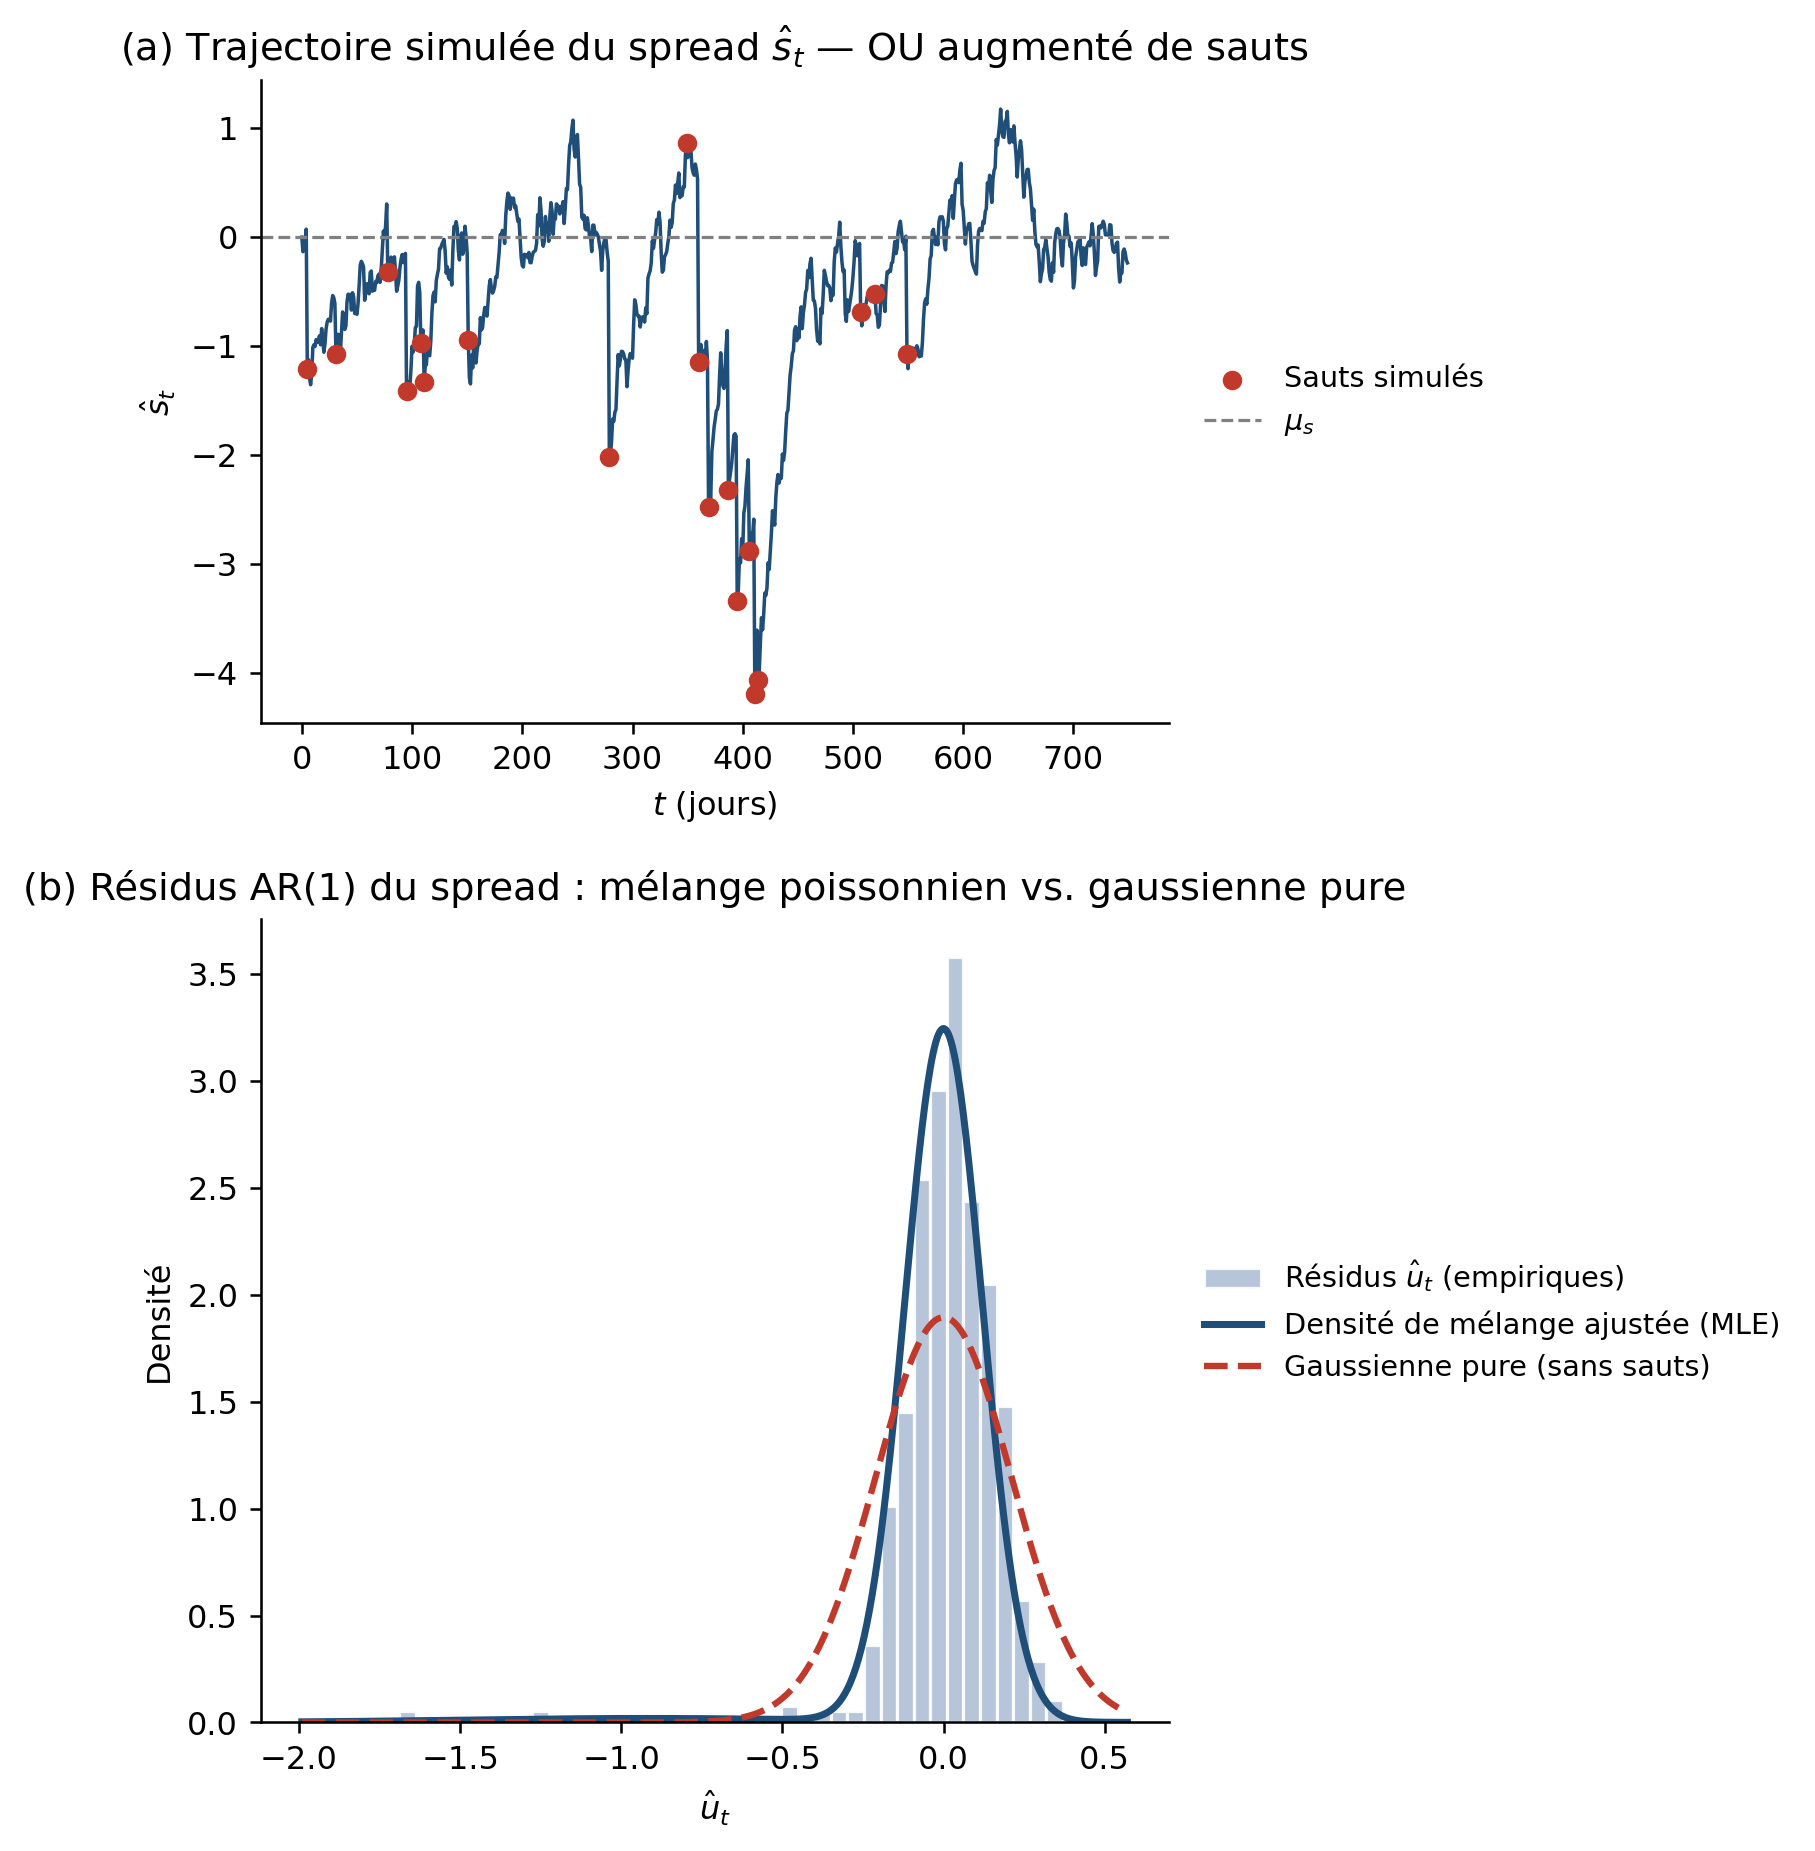
\includegraphics[width=0.85\textwidth]{fig_4_2_mixture.png}
    \caption{Estimation par maximum de vraisemblance sur un spread OU augmenté de sauts simulé ($\theta=0{,}05$, $\mu_s=0$, $\sigma_s=0{,}12$, $\lambda=0{,}025$, $\mu_J=-0{,}9$, $\sigma_J=0{,}55$, $\Delta t=1$ jour, $T=750$ jours). \textbf{(a)} Trajectoire simulée du spread $\hat s_t$, les points rouges marquant les instants de sauts effectivement tirés. \textbf{(b)} Histogramme des résidus $\hat u_t$ de la régression AR(1) naïve de la sous-partie 2.6 (qui ignore les sauts), comparé à la densité de mélange ajustée par maximum de vraisemblance (courbe pleine) et à un ajustement gaussien simple de même moyenne et variance empiriques (courbe pointillée). Le MLE récupère des paramètres proches des valeurs simulées ($\hat\lambda=0{,}026$, $\hat\mu_J=-0{,}92$, $\hat\sigma_s=0{,}120$, $\hat\sigma_J=0{,}54$). }
    \label{fig:mixture_spread}
\end{figure}
\subsection{Du paramètre estimé à la décision : le signal filtré par les sauts}
Les sous-parties 4.1 et 4.2 ont doté le spread d'un modèle complet, six paramètres $\rev{\psi}=(\theta,\mu_s,\sigma_s,\lambda,\mu_J,\sigma_J)$, et d'une méthode pour les estimer conjointement par maximum de vraisemblance. Mais une estimation ponctuelle de $\psi$, valable en moyenne sur toute la période d'estimation, ne répond pas encore à la question posée dès l'introduction : à l'instant $t$, l'écart que l'on observe est-il un bruit mean-reverting ordinaire, ou la manifestation d'un saut ? Cette sous-partie construit précisément cette réponse, sous la forme d'une probabilité calculée à chaque instant, puis l'intègre à la règle de décision du z-score posée en sous-partie 2.7.
\subsubsection*{Pourquoi une probabilité, et non une classification binaire}
On pourrait être tenté de trancher directement : au-delà d'un certain seuil, déclarer qu'un saut a eu lieu ; en-deçà, l'exclure. Une telle règle de seuil dur existe d'ailleurs, c'est la détection par seuil mentionnée en 3.7 et 4.2. Mais elle ignore une difficulté fondamentale, déjà soulignée en sous-partie 3.7 : on n'observe jamais directement \emph{si} un saut a eu lieu sur un intervalle donné, seulement l'incrément $u_t$ qui en résulte, mêlant indissociablement diffusion continue et éventuelle contribution de sauts. La bonne question n'est donc pas « y a-t-il eu un saut ? » mais « quelle est, compte tenu de $u_t$ observé, la probabilité qu'un saut ait eu lieu ? ». C'est une question de probabilité conditionnelle, et le théorème de Bayes y répond directement à partir de la densité de mélange déjà construite en sous-partie 4.2.
\subsubsection*{La probabilité a posteriori d'un saut}
On reprend l'approximation bernoullienne introduite en sous-partie 3.7 et reprise en 4.2 (au plus un saut par intervalle $\Delta t$), qui décompose la densité marginale du résidu $u_t$ en deux composantes :
\begin{equation}
f(u_t;\hat{\psi}) = \underbrace{(1-\hat\lambda\Delta t)\,\phi\!\left(u_t;\,0,\,\hat\sigma_s^2\Delta t\right)}_{\text{scénario « pas de saut »}} + \underbrace{\hat\lambda\Delta t\,\phi\!\left(u_t;\,\hat\mu_J,\,\hat\sigma_s^2\Delta t+\hat\sigma_J^2\right)}_{\text{scénario « un saut »}}
\label{eq:bernoulli_resid}
\end{equation}
où $\hat{\psi}$ désigne les paramètres estimés en sous-partie 4.2, et $\phi(\cdot;v,V^2)$ la densité gaussienne de moyenne $v$ et variance $V^2$ déjà définie en~\eqref{eq:mixture}. Chacun des deux termes de cette somme représente la contribution jointe d'un scénario (sa probabilité \emph{a priori}, $1-\hat\lambda\Delta t$ ou $\hat\lambda\Delta t$) et de la vraisemblance de $u_t$ sous ce scénario. 
Le théorème de Bayes convertit directement cette décomposition en la quantité recherchée. Par définition de la probabilité conditionnelle :
\begin{equation}
P(\text{saut sur } [t,t+\Delta t] \mid u_t) = \frac{P(u_t \mid \text{saut})\, P(\text{saut})}{P(u_t)}
\end{equation}
Le numérateur est exactement le second terme de~\eqref{eq:bernoulli_resid} (la vraisemblance de $u_t$ sous le scénario « un saut », pondérée par sa probabilité a priori $\hat\lambda\Delta t$), et le dénominateur est la densité marginale $f(u_t;\hat{\rev{\psi}})$ tout entière, la somme des deux scénarios. On obtient ainsi la \textbf{probabilité a posteriori de saut}, notée $\pi_t$ :
\begin{equation}
\pi_t \equiv P(\text{saut} \mid u_t;\hat\psi) = \frac{\hat\lambda\Delta t\,\phi\!\left(u_t;\,\hat\mu_J,\,\hat\sigma_s^2\Delta t+\hat\sigma_J^2\right)}{(1-\hat\lambda\Delta t)\,\phi\!\left(u_t;\,0,\,\hat\sigma_s^2\Delta t\right) + \hat\lambda\Delta t\,\phi\!\left(u_t;\,\hat\mu_J,\,\hat\sigma_s^2\Delta t+\hat\sigma_J^2\right)}
\label{eq:posterior_jump}
\end{equation}
Cette quantité, comprise entre $0$ et $1$, mesure la part de vraisemblance de $u_t$ attribuable au scénario « saut » plutôt qu'au scénario « diffusion pure ». Elle croît avec l'amplitude de $|u_t|$ (un résidu extrême est statistiquement plus compatible avec la composante de sauts, de variance plus large, qu'avec la diffusion seule), et avec $\hat\lambda$ et $\hat\sigma_J$ eux-mêmes : plus les sauts sont fréquents ou amples dans l'échantillon d'estimation, plus un résidu donné leur est attribué a priori.
Un point de rigueur mérite d'être signalé : rien n'empêche, en toute généralité, de reprendre cette même construction avec la densité de mélange complète~\eqref{eq:mixture_spread} tronquée à l'ordre $N$ plutôt qu'avec sa restriction bernoullienne, en calculant $P(n \mid u_t)$ pour chaque $n=0,\dots,N$ puis $\pi_t = 1-P(0\mid u_t)$. Les mêmes arguments qu'en sous-partie 3.7 (rareté des sauts, convergence à intervalle fin) justifient cependant que la restriction à $n\in\{0,1\}$ suffise en pratique, lorsque $\hat\lambda\Delta t$ est effectivement petit, avec l'avantage décisif de fournir une formule fermée pour $\pi_t$ plutôt qu'une somme tronquée à réévaluer à chaque instant.
\subsubsection*{Caractère causal du filtre}
Un point déjà rencontré à deux reprises, en sous-partie 2.7 pour $\hat\mu_s$ et $\hat{\Sigma}_s$, puis en sous-partie 2.10 pour $\hat\beta_{t|t}$, se pose à nouveau ici avec la même acuité : $\pi_t$ ne peut légitimement entrer dans une décision de trading prise à l'instant $t$ que s'il est \textbf{causal}, c'est-à-dire construit uniquement à partir d'information disponible jusqu'à $t$. Deux conditions l'assurent. D'une part, $u_t$ lui-même ne dépend que de $s_t$ et $s_{t-\Delta t}$, toutes deux observées avant ou à l'instant $t$. D'autre part, $\hat{\psi}$ doit être réestimé sur une fenêtre glissante se terminant strictement avant $t$, exactement selon la même discipline que celle imposée à $\hat\mu_s$ et $\hat{\Sigma}_s$ en sous-partie 2.7.
Cette distinction porte un nom dans la littérature économétrique des modèles à régime caché, dont la construction ci-dessus est un cas particulier : on parle de probabilité \textbf{filtrée} ($\pi_{t|t}$, n'utilisant que l'information jusqu'à $t$) par opposition à une probabilité \textbf{lissée} ($\pi_{t|T}$, qui exploiterait l'ensemble de la série, y compris les observations futures, pour ré-évaluer rétrospectivement la probabilité d'un saut à l'instant $t$). Hamilton (1989) formalise cette distinction dans le cadre plus général des modèles à changement de régime markovien, dont le modèle jump-diffusion ici retenu partage la structure sous-jacente (un état caché binaire gouvernant la loi de l'observable). La probabilité lissée, plus précise car mieux informée, n'a cependant aucune valeur opérationnelle pour une stratégie de trading en temps réel : elle correspond exactement au biais d'anticipation déjà mis en garde en sous-partie 2.7, et n'est utile qu'à des fins de diagnostic \emph{ex post}, par exemple pour examiner en fin de backtest la qualité de détection des sauts. Seule la probabilité filtrée $\pi_t$ de l'équation~\eqref{eq:posterior_jump} est mobilisée dans la règle de décision qui suit.
\subsubsection*{Le z-score structurel}
La sous-partie 4.1 a établi un résultat qu'il convient à présent d'exploiter directement : le niveau d'équilibre \emph{réellement observé} du spread, $\mu_s^{\text{eff}}=\mu_s+\lambda\mu_J/\theta$, diffère du niveau \emph{structurel} $\mu_s$ dès lors que $\mu_J\neq 0$. Le z-score de la sous-partie 2.7, $z_t=(\hat s_t-\hat\mu_s)/\hat{\Sigma}_s$, calculé à partir d'une moyenne et d'un écart-type empiriques du spread brut, est en réalité centré sur $\mu_s^{\text{eff}}$ et gonflé par la variance des sauts. On définit à la place le \textbf{z-score structurel}, construit à partir des paramètres continus isolés par l'estimation jointe de la sous-partie 4.2 :
\begin{equation}
z_t^{\text{struct}} = \frac{\hat s_t - \hat\mu_s}{\hat\sigma_s/\sqrt{2\hat\theta}}
\end{equation}
où $\hat\mu_s$ et $\hat\sigma_s$ sont ici les paramètres \emph{continus} de l'équation~\eqref{eq:ou_jump}, non contaminés par $\hat\lambda$, $\hat\mu_J$, $\hat\sigma_J$, et le dénominateur reprend l'écart-type stationnaire de la composante continue, $\sigma_s/\sqrt{2\theta}$.
\subsubsection*{La règle de décision filtrée}
La règle de décision de la sous-partie 2.7 comparait $|z_t|$ au seuil $\kappa$ sans autre considération. On lui adjoint à présent un second critère, portant sur $\pi_t$, au moyen d'un \textbf{seuil de probabilité de saut} $\pi^\ast\in(0,1)$, fixé de la même manière que $\kappa$ :
\begin{itemize}
\item \textbf{Entrée vendeuse (spread jugé trop élevé)} : $z_t^{\text{struct}} > \kappa$ \textbf{et} $\pi_t < \pi^\ast$.
\item \textbf{Entrée acheteuse (spread jugé trop bas)} : $z_t^{\text{struct}} < -\kappa$ \textbf{et} $\pi_t < \pi^\ast$.
\item \textbf{Pas d'entrée} : dès que $\pi_t \geq \pi^\ast$, quelle que soit l'amplitude de $z_t^{\text{struct}}$, l'écart observé est jugé trop probablement structurel pour qu'un pari sur son retour à la moyenne soit statistiquement fondé.
\item \textbf{Sortie sur saut détecté} : si une position est ouverte et que $\pi_t$ franchit $\pi^\ast$ en cours de vie de la position, elle est immédiatement débouclée, indépendamment des règles de sortie de la sous-partie 2.9. Ce garde-fou supplémentaire vient s'ajouter, non se substituer, aux trois règles déjà posées (retour à l'équilibre, stop sur $|z_t|$, sortie temporelle), lesquelles sont, pour la stratégie filtrée, toutes réexprimées sur $z_t^{\text{struct}}$, entrées et sorties partagent ainsi le même référentiel, ce qui évite qu'une position entre sur un z-score et sorte sur un autre, décalé de $\lambda\mu_J/\theta$.
\end{itemize}
Un choix usuel pour $\pi^\ast$ est $0{,}5$ : la position n'est ouverte que si le scénario « diffusion pure » demeure, a posteriori, plus probable que le scénario « saut ». Comme pour $\kappa$ en sous-partie 2.7, $\pi^\ast$ n'est pas estimé à partir des données mais fixé par le praticien ; sa calibration précise, par recherche sur une période de validation distincte du test final, suit la même logique que celle déjà décrite pour le ratio $Q/R$ du filtre de Kalman en sous-partie 2.10.
\subsubsection*{Ce que cette règle corrige, précisément}
Il convient de préciser exactement en quoi cette règle diffère de celle de la sous-partie 2.7, pour éviter toute ambiguïté. Le cadre gaussien pur ne peut, par construction, produire qu'un seul type de signal : un grand $|z_t|$, sans jamais distinguer sa cause. La règle filtrée introduit une seconde dimension, orthogonale à l'amplitude de l'écart : sa \emph{probable origine}. Un grand $z_t^{\text{struct}}$ accompagné d'un $\pi_t$ faible reproduit exactement la situation que la sous-partie 2.7 cherchait à capturer, un écart mean-reverting ordinaire, et se traduit par une entrée en position, désormais sur une base statistique plus assurée puisque l'hypothèse de saut a été explicitement écartée. Un grand $z_t^{\text{struct}}$ accompagné d'un $\pi_t$ élevé, en revanche, est précisément le cas que ni le z-score brut, ni le stop sur $|z_t|$ extrême de la sous-partie 2.9, ne pouvaient distinguer d'un écart normal : la règle filtrée s'abstient alors d'agir, ou clôture une position déjà ouverte, refusant de parier sur un retour à l'équilibre jugé trop risqué au regard du scénario de rupture. On soulignera enfin, le point sera décisif pour le protocole de 4.4, que la stratégie filtrée telle que définie ici diffère de la stratégie naïve par \emph{trois} modifications simultanées : (a) le filtre d'entrée $\pi_t<\pi^\ast$, (b) le remplacement du z-score naïf par $z_t^{\text{struct}}$ (centre et échelle), et (c) la règle de sortie sur saut détecté ; l'attribution du gain éventuel à chacune de ces composantes exigera une étude d'ablation.
\subsubsection*{Lien avec le contrôle périodique de cointégration}
La sous-partie 2.10 a introduit un garde-fou de nature voisine, mais agissant à une échelle de temps différente : le retest périodique du test ADF, qui suspend le trading lorsque la relation de cointégration elle-même cesse d'être valide. Le filtre de sauts $\pi_t$ opère à l'échelle de l'observation individuelle, tandis que le retest ADF opère à l'échelle de la fenêtre d'estimation tout entière ; les deux mécanismes sont complémentaires plutôt que redondants. Une accumulation de $\pi_t$ élevés sur une fenêtre récente constitue d'ailleurs un signal avant-coureur naturel qu'un retest anticipé de la cointégration, voire une réestimation complète de $\hat{\psi}$, pourrait être justifié avant même l'échéance du prochain retest programmé, une piste opérationnelle qui ne sera pas creusée davantage dans ce travail mais qui illustre la cohérence d'ensemble entre les gardes-fous des sous-parties 2.10 et 4.3.
\subsubsection*{Synthèse}
La règle filtrée ci-dessus répond précisément à la question posée en introduction : elle ne change ni le principe du pairs trading (sous-partie 2.1-2.9), ni le modèle de la dynamique du spread (sous-partie 4.1), mais conditionne la décision d'entrée à un jugement statistique explicite sur la nature de l'écart observé, jugement rendu possible par l'estimation jointe de la sous-partie 4.2. C'est cette règle filtrée, comparée à la règle naïve de la sous-partie 2.7 sur les mêmes paires et la même période, que la sous-partie 4.4 évaluera par backtest.
\begin{figure}[H]
    \centering
    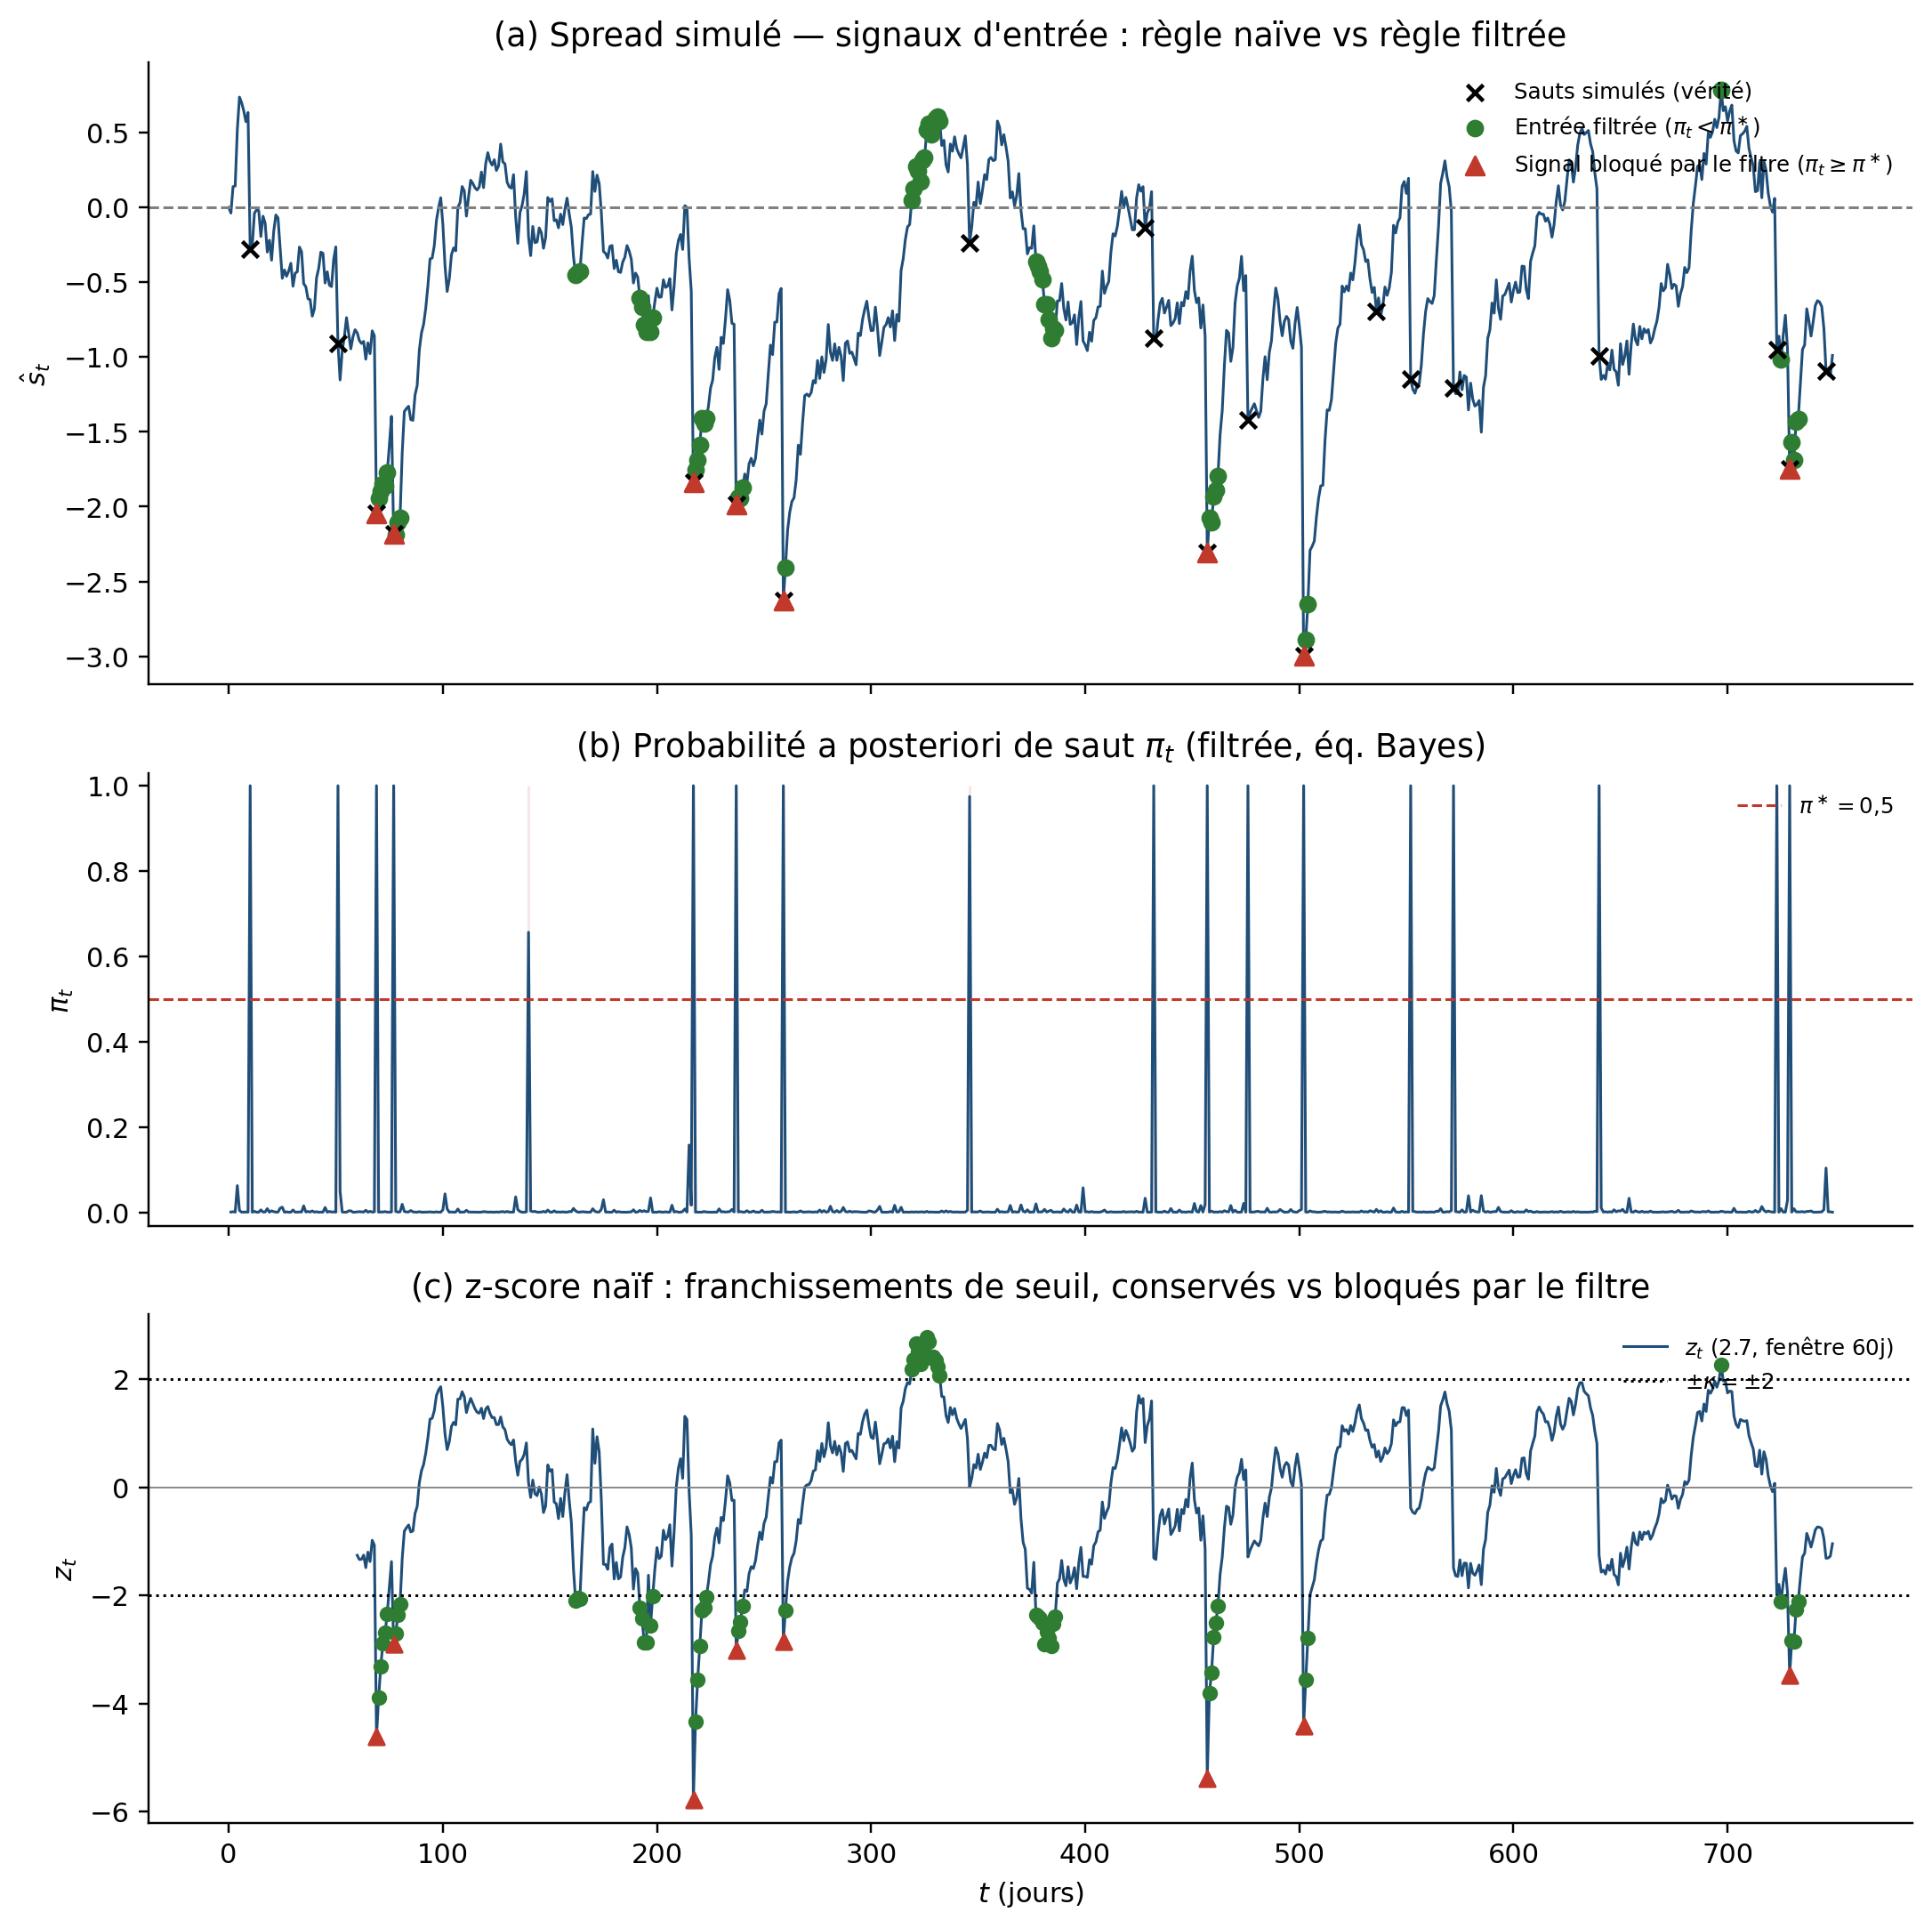
\includegraphics[width=0.9\textwidth]{fig_4_3_filtered_signal.png}
    \caption{Illustration de la règle de décision filtrée sur le spread simulé de la figure~\ref{fig:mixture_spread}. \textbf{(a)} Trajectoire du spread : les croix noires marquent les sauts effectivement simulés, les points verts les entrées conservées par le filtre ($\pi_t<\pi^\ast$), les triangles rouges les signaux que la règle naïve de la sous-partie 2.7 aurait déclenchés mais que le filtre annule ($\pi_t\geq\pi^\ast$). \textbf{(b)} Probabilité a posteriori de saut $\pi_t$ (équation~\eqref{eq:posterior_jump}) : ses pics coïncident avec les instants de sauts simulés. \textbf{(c)} z-score naïf (sous-partie 2.7, fenêtre glissante de 60 jours ; avec le seuil $\pm\kappa=\pm2$ ; mêmes signaux conservés/bloqués superposés. Sur 72 franchissements de seuil, le filtre en bloque 8, tous coïncidant avec un saut simulé.}
    \label{fig:filtered_signal}
\end{figure}
\subsection{Protocole de comparaison des stratégies}
Les sous-parties 2.7-2.9 et 4.3 ont défini deux règles de décision opérationnelles et directement comparables : une règle \textbf{naïve}, fondée uniquement sur le z-score gaussien, et une règle \textbf{filtrée}, qui lui adjoint la probabilité a posteriori de saut $\pi_t$. La figure~\ref{fig:filtered_signal} en a illustré le principe sur données simulées, où la vérité est connue. Reste à préciser le protocole rigoureux qui permettra de trancher, sur données réelles, si cette filtration améliore effectivement la performance, plutôt que de se fier à une comparaison informelle. C'est l'objet de cette sous-partie.
\subsubsection*{Les deux stratégies comparées}
Les deux stratégies, notées $\mathcal{S}_{\text{naïve}}$ et $\mathcal{S}_{\text{filtrée}}$, partagent la sélection des paires, le dimensionnement et le modèle de coûts, afin que la différence de performance observée soit imputable aux seules composantes qui les distinguent :
\begin{itemize}
\item \textbf{Commun aux deux stratégies} : sélection des paires par cointégration (2.3-2.5), estimation du hedge ratio (2.4 ou filtre de Kalman, 2.10), construction du spread (2.6), dimensionnement des positions (2.8, approche ratio $\hat\beta$), sortie temporelle par demi-vie (2.9), modèle de coûts de transaction (ci-dessous).
\item $\mathcal{S}_{\text{naïve}}$ : entrée si $|z_t|>\kappa$, sans autre condition (règle de la sous-partie 2.7, z-score sur fenêtre glissante de $W$ observations).
\item $\mathcal{S}_{\text{filtrée}}$ : entrée si $|z_t^{\text{struct}}|>\kappa$ \emph{et} $\pi_t<\pi^\ast$, avec la sortie additionnelle sur saut détecté (règle de la sous-partie 4.3).
\end{itemize}
\subsubsection*{Découpage temporel et discipline hors échantillon}
La totalité des mises en garde contre le biais d'anticipation, formulées en 2.7 pour $\hat\mu_s,\hat{\Sigma}_s$ et en 2.10 pour $\hat\beta_{t|t}$, s'appliquent à l'identique aux six paramètres $\hat{\psi}$ de la sous-partie 4.2 et à la probabilité $\pi_t$ qui en découle : leur réestimation doit être \textbf{causale}, sur une fenêtre glissante de $W$ observations se terminant strictement avant l'instant du signal. Trois découpages temporels distincts et disjoints sont nécessaires, suivant la discipline standard rappelée par López de Prado (2018) :
\begin{enumerate}
\item une période d'\textbf{entraînement}, sur laquelle les paramètres initiaux sont estimés ;
\item une période de \textbf{validation}, sur laquelle sont calibrés les hyperparamètres propres à chaque stratégie ($\kappa$, $z_{\text{exit}}$, $\kappa_{\text{stop}}$, le multiple de demi-vie, la largeur de fenêtre $W$, et, pour $\mathcal{S}_{\text{filtrée}}$ uniquement, $\pi^\ast$) ;
\item une période de \textbf{test}, sur laquelle les deux stratégies, hyperparamètres désormais figés, sont évaluées une seule fois et comparées.
\end{enumerate}
Un point mérite d'être signalé explicitement : $\pi^\ast$ ne doit en aucun cas être calibré sur la période de test elle-même, une pratique qui biaiserait mécaniquement la comparaison en faveur de $\mathcal{S}_{\text{filtrée}}$, celle-ci disposant d'un paramètre libre supplémentaire par rapport à $\mathcal{S}_{\text{naïve}}$ pour s'ajuster \emph{a posteriori} aux données de test. Le timing d'exécution suit la convention de 2.7 : signal au cours de clôture de $t$, exécution au cours de clôture de $t+1$.
\subsubsection*{Modèle de coûts de transaction}
Conformément à l'intégration des coûts dès la construction du protocole, annoncée en sous-partie 2.9, chaque exécution sur le spread supporte un coût proportionnel, appliqué séparément aux deux jambes de la position :
\begin{equation}
c_{\text{total}} = \underbrace{2\,(c_{\text{spread}} + c_{\text{commission}})\times(Q_Y P^Y_t + Q_X P^X_t)}_{\text{ouverture + clôture, sur les deux jambes}} \;+\; \underbrace{c_{\text{emprunt}}\cdot \Delta t_{\text{position}}\times(\text{notionnel de la jambe courte})}_{\text{coût de portage du short}}
\end{equation}
où $c_{\text{spread}}$ représente le demi-écart bid-ask (en proportion du notionnel), $c_{\text{commission}}$ les frais de courtage, et $c_{\text{emprunt}}$ le coût annualisé d'emprunt des titres vendus à découvert, prorata de la durée de détention $\Delta t_{\text{position}}$. 
Ces coûts sont déduits directement de la performance brute de chaque trade, pour chacune des deux stratégies indifféremment, garantissant que la comparaison porte sur des rendements nets, seuls pertinents pour juger de la valeur pratique de la filtration.
\subsubsection*{Métriques de performance}
Chaque stratégie est évaluée sur la période de test au moyen des métriques suivantes, calculées sur la série des rendements nets $\{r_t\}$ du portefeuille combiné de paires tradées :
\begin{itemize}
\item Le \textbf{ratio de Sharpe} annualisé, $\widehat{SR}=\sqrt{252}\,\hat\mu_r/\hat\sigma_r$, où $\hat\mu_r$ et $\hat\sigma_r$ sont la moyenne et l'écart-type empiriques des rendements journaliers.
\item Le \textbf{maximum drawdown}, l'ampleur de la plus grande perte cumulée depuis un sommet local de la valeur liquidative, qui mesure le risque de queue non capturé par $\hat\sigma_r$ seul.
\item Le \textbf{taux de réussite} (\emph{hit rate}), la proportion de trades clôturés en profit.
\item Le \textbf{nombre de trades} et le \textbf{turnover}, qui quantifient l'exposition cumulée aux coûts de transaction, un élément central au vu de la sous-partie 2.9 : réduire le nombre de trades, comme le fait mécaniquement $\mathcal{S}_{\text{filtrée}}$ en s'abstenant sur les signaux à forte probabilité de saut, réduit \emph{à performance brute égale} les coûts cumulés.
\item La \textbf{durée moyenne de détention}, à comparer à la demi-vie $t_{1/2}$ de la sous-partie 2.6, comme test de cohérence entre la théorie et le comportement réalisé de la stratégie.
\end{itemize}
\subsubsection*{Tester la significativité de la différence de Sharpe}
Un écart de ratio de Sharpe observé entre $\mathcal{S}_{\text{naïve}}$ et $\mathcal{S}_{\text{filtrée}}$ sur un unique échantillon de test ne suffit pas, en lui-même, à conclure : il faut encore déterminer s'il excède ce que le bruit d'échantillonnage peut expliquer. Un test $t$ usuel pour échantillons indépendants serait ici inadapté : les deux stratégies tradent les mêmes paires, sur la même période, et leurs rendements $r_t^{\text{naïve}}$ et $r_t^{\text{filtrée}}$ sont donc fortement corrélés au jour le jour, une corrélation qu'un test d'indépendance ignorerait à tort.
Jobson et Korkie (1981), dans la correction proposée par Memmel (2003), fournissent un test adapté à la comparaison de deux ratios de Sharpe calculés sur des rendements corrélés. En notant $\hat\mu_A,\hat\sigma_A$ et $\hat\mu_B,\hat\sigma_B$ les moyennes et écarts-types empiriques des deux séries de rendements avec la convention explicite $A=\mathcal{S}_{\text{naïve}}$, $B=\mathcal{S}_{\text{filtrée}}$, de sorte que $\hat z<0$ signifie un Sharpe supérieur pour la stratégie filtrée, et $\hat\sigma_{AB}$ leur covariance empirique, la statistique de test s'écrit :
\begin{equation}
\hat z = \frac{\hat\sigma_B\hat\mu_A - \hat\sigma_A\hat\mu_B}{\sqrt{\hat{V}}}
\end{equation}
avec la variance asymptotique corrigée :
\begin{equation}
\hat{V} = \frac{1}{T}\left(2\hat\sigma_A^2\hat\sigma_B^2 - 2\hat\sigma_A\hat\sigma_B\hat\sigma_{AB} + \frac{1}{2}\hat\mu_A^2\hat\sigma_B^2 + \frac{1}{2}\hat\mu_B^2\hat\sigma_A^2 - \frac{\hat\mu_A\hat\mu_B}{\hat\sigma_A\hat\sigma_B}\hat\sigma_{AB}^2\right)
\end{equation}
Cette expression s'obtient par la méthode delta, appliquée conjointement aux deux ratios $\hat\mu_A/\hat\sigma_A$ et $\hat\mu_B/\hat\sigma_B$ à partir de la loi asymptotique jointe des quatre moments empiriques $(\hat\mu_A,\hat\sigma_A,\hat\mu_B,\hat\sigma_B)$, exactement le même principe de linéarisation autour du maximum déjà mobilisé pour établir la loi asymptotique du rapport de vraisemblance en sous-partie 3.7. Sous $H_0: SR_A=SR_B$, $\hat z$ suit asymptotiquement une loi $\mathcal{N}(0,1)$, ce qui permet un test bilatéral usuel au seuil choisi.
\paragraph{Justification par la méthode delta.}
Cette expression n'est pas postulée mais se dérive rigoureusement, par la méthode delta multivariée, à partir de la loi asymptotique jointe des quatre moments empiriques $(\hat\mu_A,\hat\sigma_A,\hat\mu_B,\hat\sigma_B)$, sous l'hypothèse usuelle (celle de Jobson et Korkie) que les rendements des deux stratégies sont conjointement gaussiens.
\paragraph{Rappel : la méthode delta multivariée.} Si $\sqrt{T}(\hat\vartheta-\vartheta) \xrightarrow{d} \mathcal{N}(0,\Sigma)$ pour un vecteur de paramètres $\vartheta$, et si $g$ est différentiable en $\vartheta$, alors :
\begin{equation}
\sqrt{T}\left(g(\hat\vartheta)-g(\vartheta)\right) \xrightarrow{d} \mathcal{N}\!\left(0,\ \nabla g(\vartheta)^\top \Sigma\, \nabla g(\vartheta)\right)
\end{equation}
C'est exactement le même principe de linéarisation autour du vrai paramètre, par développement de Taylor à l'ordre 1, que celui déjà mobilisé pour la loi asymptotique du rapport de vraisemblance en sous-partie 3.7, ici appliqué non à la log-vraisemblance, mais directement à la fonction $g(\mu_A,\sigma_A,\mu_B,\sigma_B) = \sigma_B\mu_A - \sigma_A\mu_B$, dont $\hat g = \hat\sigma_B\hat\mu_A-\hat\sigma_A\hat\mu_B$ est l'estimateur au numérateur de $\hat z$.
\paragraph{Étape 1 -- Variance et covariance des moyennes empiriques.} Ce sont les résultats les plus directs, conséquence immédiate du théorème central limite appliqué à $\hat\mu_A=\frac{1}{T}\sum_t r_t^A$ et $\hat\mu_B=\frac{1}{T}\sum_t r_t^B$ :
\begin{equation}
\text{Var}(\hat\mu_A) = \frac{\sigma_A^2}{T}, \qquad \text{Var}(\hat\mu_B) = \frac{\sigma_B^2}{T}, \qquad \text{Cov}(\hat\mu_A,\hat\mu_B) = \frac{\sigma_{AB}}{T}
\end{equation}
\paragraph{Étape 2 -- Variance de l'écart-type empirique.} Sous normalité, $(T-1)\hat\sigma_A^2/\sigma_A^2 \sim \chi^2_{T-1}$, dont la variance vaut $2(T-1)$. On en déduit :
\begin{equation}
\text{Var}(\hat\sigma_A^2) = \frac{\sigma_A^4}{(T-1)^2}\cdot 2(T-1) = \frac{2\sigma_A^4}{T-1} \approx \frac{2\sigma_A^4}{T}
\end{equation}
La méthode delta, appliquée cette fois à la transformation $x\mapsto\sqrt{x}$ (de dérivée $1/(2\sqrt{x})$), convertit cette variance de $\hat\sigma_A^2$ en variance de $\hat\sigma_A$ :
\begin{equation}
\text{Var}(\hat\sigma_A) \approx \left(\frac{1}{2\sigma_A}\right)^2 \text{Var}(\hat\sigma_A^2) = \frac{1}{4\sigma_A^2}\cdot\frac{2\sigma_A^4}{T} = \frac{\sigma_A^2}{2T}
\end{equation}
et de façon identique $\text{Var}(\hat\sigma_B)=\sigma_B^2/(2T)$.
\paragraph{Étape 3 -- Covariance entre les deux écarts-types empiriques.} Il faut d'abord établir $\text{Cov}(\hat\sigma_A^2,\hat\sigma_B^2)$. Pour $(X,Y)$ bivariées gaussiennes centrées de covariance $\sigma_{XY}$, on écrit la décomposition de régression, valide pour tout couple gaussien conjoint : $Y=\beta X+\varepsilon$, avec $\beta=\sigma_{XY}/\sigma_X^2$ et $\varepsilon\sim\mathcal{N}(0,\sigma_\varepsilon^2)$ indépendant de $X$, où $\sigma_\varepsilon^2=\sigma_Y^2-\sigma_{XY}^2/\sigma_X^2$. En développant $X^2Y^2=X^2(\beta X+\varepsilon)^2$ et en utilisant $E[X^4]=3\sigma_X^4$ (moment d'ordre 4 d'une gaussienne centrée) ainsi que l'indépendance de $\varepsilon$ et $X$ :
\begin{align}
E[X^2Y^2] &= \beta^2 E[X^4] + 2\beta E[X^3\varepsilon] + E[X^2]\,E[\varepsilon^2] \\
&= \beta^2\cdot 3\sigma_X^4 + 2\beta\,E[X^3]E[\varepsilon] + \sigma_X^2\sigma_\varepsilon^2 = \beta^2\cdot 3\sigma_X^4 + 0 + \sigma_X^2\sigma_\varepsilon^2\\
&= 3\sigma_{XY}^2 + \sigma_X^2\left(\sigma_Y^2-\frac{\sigma_{XY}^2}{\sigma_X^2}\right) = \sigma_X^2\sigma_Y^2 + 2\sigma_{XY}^2
\end{align}
D'où, puisque $E[X^2]E[Y^2]=\sigma_X^2\sigma_Y^2$ :
\begin{equation}
\text{Cov}(X^2,Y^2) = E[X^2Y^2]-E[X^2]E[Y^2] = 2\sigma_{XY}^2
\end{equation}
Appliqué aux écarts-types empiriques (par le même argument de $\chi^2$ que pour l'étape 2, transposé au cas bivarié) :
\begin{equation}
\text{Cov}(\hat\sigma_A^2,\hat\sigma_B^2) \approx \frac{2\sigma_{AB}^2}{T}
\end{equation}
puis, par la méthode delta bivariée appliquée à $\sqrt{\cdot}$ sur chacune des deux composantes :
\begin{equation}
\text{Cov}(\hat\sigma_A,\hat\sigma_B) \approx \frac{1}{2\sigma_A}\cdot\frac{1}{2\sigma_B}\cdot\text{Cov}(\hat\sigma_A^2,\hat\sigma_B^2) = \frac{\sigma_{AB}^2}{2\sigma_A\sigma_B\, T}
\end{equation}
\paragraph{Étape 4 -- Indépendance entre moyennes et écarts-types.} Un résultat classique de la théorie gaussienne multivariée (indépendance du vecteur des moyennes empiriques et de la matrice de covariance empirique pour un échantillon i.i.d. gaussien) donne, à l'ordre asymptotique considéré :
\begin{equation}
\text{Cov}(\hat\mu_A,\hat\sigma_A)=\text{Cov}(\hat\mu_A,\hat\sigma_B)=\text{Cov}(\hat\mu_B,\hat\sigma_A)=\text{Cov}(\hat\mu_B,\hat\sigma_B)=0
\end{equation}
Cette propriété découle du fait que, pour un échantillon gaussien i.i.d., la vraisemblance se factorise en un terme ne dépendant que de $\hat\mu$ et un terme ne dépendant que des écarts à $\hat\mu$ -- une conséquence directe du théorème de Basu appliqué à la statistique exhaustive et complète $\hat\mu$. Le bloc « moyennes » et le bloc « écarts-types » de la matrice de covariance asymptotique sont ainsi mutuellement orthogonaux.
\paragraph{Étape 5 -- Le gradient de $g$.} Pour $g(\mu_A,\sigma_A,\mu_B,\sigma_B)=\sigma_B\mu_A-\sigma_A\mu_B$ :
\begin{equation}
\frac{\partial g}{\partial \mu_A}=\sigma_B, \qquad \frac{\partial g}{\partial \sigma_A}=-\mu_B, \qquad \frac{\partial g}{\partial \mu_B}=-\sigma_A, \qquad \frac{\partial g}{\partial \sigma_B}=\mu_A
\end{equation}
\paragraph{Étape 6 -- Assemblage.} La variance asymptotique de $\hat g$ se décompose, grâce à l'orthogonalité établie à l'étape 4, en la somme de deux formes quadratiques indépendantes, l'une sur le bloc des moyennes, l'autre sur le bloc des écarts-types :
\begin{align}
\text{Var}(\hat g) &\approx \underbrace{\sigma_B^2\,\text{Var}(\hat\mu_A) + \sigma_A^2\,\text{Var}(\hat\mu_B) - 2\sigma_A\sigma_B\,\text{Cov}(\hat\mu_A,\hat\mu_B)}_{\text{bloc moyennes}} \notag \\
&\quad + \underbrace{\mu_B^2\,\text{Var}(\hat\sigma_A) + \mu_A^2\,\text{Var}(\hat\sigma_B) - 2\mu_A\mu_B\,\text{Cov}(\hat\sigma_A,\hat\sigma_B)}_{\text{bloc écarts-types}}
\end{align}
où les signes négatifs proviennent directement du produit des dérivées partielles de signes opposés, $\sigma_B\cdot(-\sigma_A)$ pour le premier bloc et $(-\mu_B)\cdot\mu_A$ pour le second. En substituant les résultats des étapes 1 à 3 :
\begin{align}
\text{bloc moyennes} &= \sigma_B^2\frac{\sigma_A^2}{T} + \sigma_A^2\frac{\sigma_B^2}{T} - 2\sigma_A\sigma_B\frac{\sigma_{AB}}{T} = \frac{1}{T}\left(2\sigma_A^2\sigma_B^2 - 2\sigma_A\sigma_B\sigma_{AB}\right) \\
\text{bloc écarts-types} &= \mu_B^2\frac{\sigma_A^2}{2T} + \mu_A^2\frac{\sigma_B^2}{2T} - 2\mu_A\mu_B\frac{\sigma_{AB}^2}{2\sigma_A\sigma_B\, T} = \frac{1}{T}\left(\frac{1}{2}\mu_A^2\sigma_B^2 + \frac{1}{2}\mu_B^2\sigma_A^2 - \frac{\mu_A\mu_B}{\sigma_A\sigma_B}\sigma_{AB}^2\right)
\end{align}
En sommant les deux blocs, on retrouve exactement $\text{Var}(\hat g)\approx\hat{\rev{V}}$ tel que défini plus haut : chaque terme de $\hat{V}$ s'identifie ainsi précisément à sa source, covariance des moyennes pour les deux premiers termes, covariance des écarts-types pour les trois derniers, sans qu'aucun terme supplémentaire n'intervienne.
\subsubsection*{Robustesse par régime de marché}
Une performance agrégée sur toute la période de test peut masquer une hétérogénéité importante : la valeur ajoutée du filtre de sauts n'a, par construction, de raison de se manifester que lorsque des sauts sont effectivement présents dans les données, une fréquence qui peut elle-même varier avec le régime de marché. Le protocole segmente donc la période de test en sous-périodes homogènes, bull market, bear market, marché latéral et périodes de forte volatilité, par exemple à partir de la tendance et de la volatilité réalisée d'un indice de référence, et répète l'ensemble des comparaisons ci-dessus indépendamment sur chaque segment. Cette décomposition permet de vérifier une hypothèse naturelle, déjà suggérée par la nature même du modèle de sauts : que l'écart de performance entre $\mathcal{S}_{\text{filtrée}}$ et $\mathcal{S}_{\text{naïve}}$ soit concentré dans les périodes de forte volatilité ou de rupture, où le risque de confondre un saut avec un écart mean-reverting ordinaire est le plus élevé, et faible ou nul dans les régimes calmes, où les deux stratégies devraient, par construction, converger vers un comportement quasi identique.
\subsubsection*{Synthèse}
Ce protocole complète, par un cadre de test rigoureux, la construction méthodologique des sous-parties 4.1 à 4.3 : un modèle (4.1), une méthode pour l'estimer (4.2), une règle de décision qui en découle (4.3), et à présent un protocole permettant de juger objectivement si cette dernière améliore la performance d'une stratégie de pairs trading, la question posée dès l'introduction de ce travail. Les résultats de son application aux données réelles font l'objet des sous-parties suivantes.
\subsection{Univers de paires, sélection et biais associés}
Le protocole de la sous-partie 4.4 suppose implicitement un ensemble de paires déjà constitué, sur lequel les deux stratégies sont comparées. Cette étape, en apparence préliminaire, est en réalité l'une des plus exposées aux biais de backtest annoncés dès la description de ce travail : la manière dont les paires sont choisies peut, à elle seule, produire une performance apparente qui ne doit rien à la stratégie elle-même. Cette sous-partie détaille l'univers de départ, la procédure de sélection, et les biais qu'il convient explicitement de neutraliser avant toute comparaison.
\subsubsection*{L'univers de départ}
L'univers candidat est constitué d'actions appartenant à un même secteur ou sous-secteur d'activité, sur le principe économique posé dès l'introduction : deux entreprises exposées aux mêmes chocs fondamentaux (prix des intrants, réglementation, cycle de demande) sont plus susceptibles d'entretenir une relation d'équilibre de long terme stable que deux entreprises choisies au hasard. La paire Mastercard/Visa (MA/V), appartient à ce type de construction : deux réseaux de paiement directement concurrents, structurellement exposés aux mêmes déterminants macroéconomiques (volume de transactions par carte, dépenses de consommation).
\subsubsection*{Fenêtre de formation et fenêtre de trading}
Une erreur méthodologique fréquente consiste à sélectionner les paires par cointégration sur l'ensemble de la période disponible, y compris la période sur laquelle la stratégie est ensuite testée, un cas particulier du biais d'anticipation déjà mis en garde à plusieurs reprises (sous-parties 2.7, 2.10, 4.4). Une paire jugée cointégrée sur toute la période, y compris la période de test, l'est potentiellement \emph{parce que} son comportement sur la période de test a contribué à la valider, ce qui invalide la logique même du test hors échantillon.
Gatev, Goetzmann et Rouwenhorst (2006) formalisent la solution standard, retenue ici : une \textbf{fenêtre de formation}, sur laquelle la cointégration est testée et les paires retenues, strictement antérieure et disjointe d'une \textbf{fenêtre de trading}, sur laquelle les stratégies sont effectivement évaluées. Cette discipline reproduit, à l'échelle de la sélection des paires plutôt qu'à celle de l'estimation des paramètres, exactement le découpage entraînement/validation/test déjà posé en sous-partie 4.4.
\subsubsection*{Critères de sélection}
Une paire candidate est retenue pour la fenêtre de trading suivante si, sur la fenêtre de formation qui la précède, elle satisfait simultanément :
\begin{itemize}
\item la confirmation préalable que chacun des deux log-prix est $I(1)$ (étape zéro de la sous-partie 2.5) ;
\item le rejet de l'hypothèse nulle du test ADF sur le spread, au seuil retenu ;
\item une demi-vie $t_{1/2}$ (sous-partie 2.6, corrigée du biais d'échantillon fini) comprise dans une fourchette raisonnable, ni trop courte (quelques jours, où le bruit de microstructure et les coûts de transaction dominent le signal) ni trop longue (plusieurs mois, où le capital est immobilisé sans certitude que la relation d'équilibre perdure) ;
\item un historique de cotation suffisant pour que l'estimation des six paramètres du modèle jump-diffusion (sous-partie 4.2) dispose d'assez d'observations pour être fiable.
\end{itemize}
\subsubsection*{Le biais de sélection multiple}
Même en respectant scrupuleusement le découpage formation/trading, un second biais, plus subtil, subsiste : si l'univers candidat comporte $N$ paires, tester chacune au seuil $\alpha$ produit, sous l'hypothèse nulle où \emph{aucune} de ces paires n'est en réalité cointégrée, un nombre \emph{attendu} de faux positifs égal à $N\alpha$. Pour un secteur de $40$ titres, par exemple, le nombre de paires candidates est $\binom{40}{2}=780$ ; à $\alpha=5\%$, on attend en moyenne $780\times0{,}05\approx 39$ paires jugées à tort cointégrées, uniquement par le hasard de l'échantillonnage, avant même d'avoir examiné une seule vraie relation économique. Ce phénomène, documenté de façon générale par Harvey, Liu et Zhu (2016) dans le contexte plus large de la découverte de facteurs de risque, s'applique à l'identique à la sélection de paires par test statistique répété.
Deux corrections usuelles permettent de contrôler ce risque. La correction de \textbf{Bonferroni}, la plus conservatrice, ajuste le seuil individuel à $\alpha/N$ de sorte que la probabilité de commettre \emph{au moins une} fausse découverte sur l'ensemble des $N$ tests reste bornée par $\alpha$. Moins conservatrice, la procédure de contrôle du \textbf{taux de fausses découvertes} (\emph{false discovery rate}, FDR) de Benjamini et Hochberg (1995) ordonne les $N$ $p$-valeurs $p_{(1)}\leq\dots\leq p_{(N)}$ et retient toutes les paires jusqu'au rang $k^\ast$ défini par :
\begin{equation}
k^\ast = \max\left\{k : p_{(k)} \leq \frac{k}{N}\,\alpha\right\}
\end{equation}
garantissant que la \emph{proportion attendue} de fausses découvertes parmi les paires retenues, plutôt que la probabilité d'en commettre ne serait-ce qu'une seule, reste bornée par $\alpha$. Cette garantie suppose toutefois l'indépendance des tests, ou une dépendance positive (PRDS, au sens de Benjamini et Yekutieli, 2001) ; or les tests de paires d'un même secteur sont fortement dépendants par construction --- chaque titre apparaît dans $39$ paires, et les $p$-valeurs partagent les mêmes chocs. Sous dépendance arbitraire, la variante de Benjamini-Yekutieli (facteur correctif $\sum_{k=1}^N 1/k$), plus conservatrice, est celle qui conserve la garantie ; c'est elle qui est retenue ici, un compromis mieux adapté à ce travail, où l'objectif est de disposer d'un nombre suffisant de paires pour que la comparaison de stratégies de la sous-partie 4.4 dispose d'une puissance statistique raisonnable, plutôt que d'isoler la seule paire la plus significative.
\subsubsection*{Le biais de survivance}
Un univers construit à partir des seules entreprises \emph{actuellement} cotées, comme c'est le cas de la paire MA/V utilisée à titre illustratif dans ce travail, souffre potentiellement d'un \textbf{biais de survivance} (\emph{survivorship bias}) : les entreprises ayant fait faillite, ayant été retirées de la cote, ou ayant fusionné durant la période étudiée sont, par construction, absentes de l'univers reconstitué a posteriori, alors qu'elles auraient fait partie de l'univers réellement disponible pour un investisseur à l'époque considérée. Ce biais, documenté de façon générale par Elton, Gruber et Blake (1996), tend à surestimer la performance de toute stratégie backtestée sur un tel univers, puisque les paires impliquant une entreprise en difficulté, potentiellement plus susceptibles de connaître une rupture structurelle de leur relation de cointégration, précisément le phénomène que ce travail cherche à détecter via $\pi_t$, sont mécaniquement absentes de l'échantillon. La correction rigoureuse exige un univers \emph{point-in-time}, reconstituant la composition réelle du secteur à chaque date de formation ; ce travail, faute d'accès à une base de données point-in-time, se limite à signaler explicitement cette limite plutôt que de la dissimuler, conformément à l'exigence de rigueur expérimentale annoncée dès l'introduction de ce travail.
\subsubsection*{Réestimation périodique de l'univers}
Une paire cointégrée sur une fenêtre de formation donnée ne le demeure pas nécessairement indéfiniment, un phénomène déjà anticipé en sous-partie 2.10 par le retest périodique du test ADF au cours du trading. Par cohérence, l'univers de paires lui-même est reconstitué à intervalles réguliers : à chaque nouvelle fenêtre de formation, l'ensemble de la procédure ci-dessus (test ADF, critères de demi-vie, correction pour tests multiples) est réappliqué, et la liste des paires tradées sur la fenêtre de trading suivante est mise à jour en conséquence, plutôt que figée une fois pour toutes au début du backtest.
\subsubsection*{Données utilisées dans cette étude}
Les données de prix utilisées sont les cours de clôture ajustés (dividendes et fractionnements inclus), à fréquence journalière, obtenus via Yahoo Finance. La paire MA/V a servi de validation de bout en bout du protocole, de l'estimation du hedge ratio (2.4) jusqu'au test du rapport de vraisemblance sur les sauts (4.2), cette validation étant conduite exclusivement sur la fenêtre de formation 2014-2018. Le test du rapport de vraisemblance y rejette l'absence de sauts sur la fenêtre de formation ($\Lambda\approx 270$, largement au-delà de toute valeur critique plausible --- conclusion robuste malgré les réserves de 3.7 sur la distribution de référence $\chi^2_2$), confirmant sur données réelles la pertinence empirique du cadre construit en partie 4. Ce travail sera étendu, dans la sous-partie 4.6, à un univers plus large de paires sectorielles construit selon la procédure de sélection ci-dessus, seule échelle permettant une comparaison statistiquement informative des deux stratégies au sens du test de la sous-partie 4.4.
\subsubsection*{Synthèse}
Cette sous-partie a précisé les fondations empiriques sur lesquelles repose la comparaison de stratégies : un univers sectoriel, un découpage formation/trading disjoint pour éviter le biais d'anticipation dans la sélection elle-même, une correction explicite pour les tests multiples (Benjamini-Yekutieli, valide sous dépendance), une reconnaissance du biais de survivance non corrigé, et un principe de réestimation périodique cohérent avec celui déjà retenu pour les paramètres du modèle. La sous-partie 4.6 applique désormais l'ensemble de cet appareillage, modèle, estimation, signal filtré, protocole de comparaison et univers de paires, pour trancher empiriquement la question posée dès l'introduction de ce travail.
\subsection{Résultats empiriques : comparaison des stratégies}
Les sections 4.1 à 4.5 ont construit, étape par étape, le cadre théorique complet : modélisation du spread par un processus d'Ornstein--Uhlenbeck à sauts (éq.~\eqref{eq:ou_jump}), estimation MLE des six paramètres $(\theta,\mu_s,\sigma_s,\lambda,\mu_J,\sigma_J)$ par la méthode de Ball--Torous, calcul de la probabilité a posteriori de saut $\pi_t$ (éq.~\eqref{eq:posterior_jump}), règle de décision filtrée conditionnant l'entrée en position à $\pi_t<\pi^\ast$, protocole de comparaison naïve/filtrée par le test de Jobson--Korkie/Memmel (contrôlé par Ledoit-Wolf), et discussion critique de la sélection de l'univers de paires. Cette dernière sous-partie applique l'ensemble du protocole à des données réelles, afin de vérifier si le filtrage des sauts produit un gain de performance mesurable une fois les coûts de transaction pris en compte.
\subsubsection*{Protocole implémenté}
Conformément à 4.4, l'échantillon est scindé en une \emph{fenêtre de formation} (01/01/2014 -- 31/12/2018, cinq ans) sur laquelle sont estimés les ordres d'intégration des deux log-prix (étape zéro), le ratio de couverture $\hat\beta$ (régression OLS des log-prix), le test ADF d'Engle--Granger sur le spread (valeurs critiques de MacKinnon pour résidus estimés), la régression AR(1) fournissant $(\hat\theta,\hat\mu_s,\hat\sigma_s)$, puis l'ajustement MLE des paramètres de saut $(\hat\lambda,\hat\mu_J,\hat\sigma_J)$ et le test du rapport de vraisemblance de la section 3.7 ; et une \emph{fenêtre de trading} (01/01/2019 -- 31/12/2024, six ans) sur laquelle les deux stratégies, naïve (règle d'entrée de la section 2.7, seuil $\kappa=2$) et filtrée (règle de la section 4.3, seuil $\pi^\ast=0{,}5$) sont simulées jour par jour, en n'utilisant \emph{que} les paramètres estimés sur la formation (aucune ré-estimation glissante n'est appliquée ici, contrairement à la recommandation de la section 2.10 ; ce choix, dicté par la nécessité de conserver un protocole simple et reproductible, est discuté plus bas comme une limite, de même que l'absence de période de validation intermédiaire : contrairement au découpage en trois blocs prescrit en 4.4, les hyperparamètres $(\kappa,\pi^\ast)$ sont ici fixés par convention a priori et non calibrés, l'analyse de sensibilité de 4.7, conduite sur la période de test, ne s'y substitue pas et impose le recours au Deflated Sharpe Ratio). Un coût de transaction proportionnel de $10$ points de base par jambe et par exécution est appliqué à l'ouverture et à la clôture de chaque position, conformément à l'ordre de grandeur usuel pour des actions liquides du S\&P~500.
Une position de pairs trading n'est jamais unijambiste : elle repose sur deux positions simultanées et opposées, formant les deux \emph{jambes} du trade. Si le spread $s_t=\ln P_A-\beta\ln P_B$ est jugé excessivement élevé, on anticipe son resserrement en vendant à découvert le titre $A$ (jambe courte) et en achetant $\beta$ dollars de notionnel du titre $B$ par dollar court de $A$ (jambe longue) ; le cas symétrique (spread excessivement bas) inverse les deux jambes. Chaque jambe correspondant à une exécution de marché distincte, elle supporte son propre coût de transaction : ouvrir la position coûte ainsi $2\times\text{COST}$ (une exécution sur chaque titre), et son dénouement ultérieur en coûte à nouveau $2\times\text{COST}$, soit un frottement total de $4\times\text{COST}$ par aller-retour complet. Cette construction à deux jambes, en éliminant par différence les mouvements communs de marché ou de secteur affectant $A$ et $B$, est précisément ce qui confère à la stratégie son caractère \emph{market-neutral} introduit en 2.1.
Faute d'un univers sectoriel large et d'une procédure de correction pour sélection multiple telle que décrite en 4.5, l'exercice se limite ici à trois paires choisies pour leur cointégration documentée sur des fenêtres antérieures : \texttt{MA/V} (paiements), \texttt{XOM/CVX} (énergie intégrée) et \texttt{HD/LOW} (distribution spécialisée). Le portefeuille agrégé est équipondéré entre les trois paires.
\subsubsection*{Diagnostics de la fenêtre de formation}
\begin{center}
\begin{tabular}{lccccc}
\toprule
Paire & $\hat\beta$ & $p_{\text{ADF}}$ & Demi-vie (j) & $\hat\lambda$ (j$^{-1}$) & $p_{\text{LR}}$ \\
\midrule
MA / V & 1{,}044 & 0{,}1147 & 76{,}4 & 0{,}152 & $<10^{-4}$ \\
XOM / CVX & 0{,}281 & 0{,}1102 & 54{,}7 & 0{,}714 & $<10^{-4}$ \\
HD / LOW & 1{,}235 & 0{,}1164 & 57{,}9 & 0{,}093 & $<10^{-4}$ \\
\bottomrule
\end{tabular}
\end{center}
(Les $p_{\text{ADF}}$ sont calculées sous la distribution d'Engle-Granger/MacKinnon pour résidus estimés ; les $p_{\text{LR}}$ sous la référence $\chi^2_2$, indicative au vu des réserves de 3.7 --- les valeurs de $\Lambda$ obtenues excèdent toutefois de plusieurs ordres de grandeur toute valeur critique plausible, y compris bootstrapée.)
Deux constats s'imposent. D'une part, le test du rapport de vraisemblance rejette systématiquement et très fortement l'hypothèse d'absence de sauts ($p<10^{-4}$ pour les trois paires) : la composante de saut n'est pas un artefact de spécification, elle est statistiquement dominante sur la fenêtre de formation, ce qui justifie a posteriori la démarche de filtrage. L'intensité estimée pour XOM/CVX, $\hat\lambda=0{,}714$ par jour, appelle toutefois une mise en garde spécifique : elle correspond à un \og saut \fg{} tous les 1{,}4 jours ouvrés, soit environ 180 par an, une fréquence incompatible avec l'interprétation des sauts comme événements d'information \emph{rares} (3.7), et qui suggère que la composante de sauts absorbe ici la kurtosis ordinaire des rendements (volatilité stochastique) plutôt que des discontinuités véritables. Elle invalide en outre, pour cette paire, l'approximation bernoullienne utilisée dans $\pi_t$ ($P(N\geq 2)\approx 12\,\%$ par intervalle) et élève le prior de saut au point que le filtre devrait y bloquer une fraction importante des entrées ; la version complète \eqref{eq:mixture_spread}, tronquée à l'ordre $N$, est donc utilisée pour cette paire en lieu et place de la formule fermée bernoullienne, et l'interprétation économique de $\hat\lambda$ y est traitée avec prudence. Un modèle à volatilité stochastique et sauts (SVJD), ou à intensité variable, serait mieux adapté, extension laissée aux perspectives. D'autre part, et c'est le point qui doit être signalé avec la même rigueur, \emph{aucune des trois paires ne rejette l'hypothèse nulle de racine unitaire au seuil conventionnel de 5\,\% sur cette fenêtre de cinq ans} ($p\in[0{,}110\,;\,0{,}117]$) : au sens strict du critère de sélection formulé en 4.5, aucune ne serait retenue.
Ce résultat n'est pas anecdotique et mérite d'être interprété plutôt qu'ignoré. L'explication avancée dans la version initiale de ce travail, une fenêtre de cinq ans \og trop longue \fg{} pour la puissance du test ADF, était économétriquement inversée et doit être corrigée : la puissance du test ADF \emph{croît} avec la longueur de l'échantillon rapportée à la demi-vie (elle est faible quand la demi-vie est longue \emph{relativement} à l'échantillon). Or, avec des demi-vies estimées de 54 à 76 jours et un échantillon d'environ 1\,260 jours, la fenêtre de formation contient une vingtaine de demi-vies : si le spread était réellement un AR(1) stationnaire conforme à ces estimations, le test rejetterait $H_0$ avec une probabilité proche de 1. Les $p$-valeurs de l'ordre de 0{,}11 indiquent donc autre chose : soit la demi-vie réelle est nettement plus longue que la demi-vie estimée (cohérent avec le biais d'échantillon fini de $\hat\phi$, qui sous-estime systématiquement $t_{1/2}$, cf. 2.6), soit la relation a dérivé au cours des cinq ans (instabilité de $\beta$, au sens de 2.10), soit la cointégration est tout simplement absente. Chacune de ces trois lectures affaiblit la validité des paires retenues.
Deux attitudes étaient possibles face à ce constat : écarter silencieusement ces trois paires et n'en présenter que d'autres qui satisferaient le critère strict, ou documenter honnêtement la situation et poursuivre l'exercice à titre illustratif en signalant la limite. C'est la seconde option qui est retenue ici, dans la continuité de la discussion de 4.5 sur le biais de sélection : les résultats qui suivent doivent donc être lus comme une \emph{démonstration du protocole} sur des paires plausibles mais non rigoureusement validées par le critère de sélection qu'elles sont censées satisfaire, et non comme la preuve qu'une stratégie tradable a été identifiée.
\subsubsection*{Performance agrégée sur la fenêtre de trading}
\begin{center}
\begin{tabular}{lccccc}
\toprule
Stratégie & Sharpe annualisé & Drawdown max & Nb. trades & Taux de succès & Durée moy. (j) \\
\midrule
Naïve (2.7) & $+0{,}036$ & $-30{,}1\,\%$ & 73 & 65{,}7\,\% & 36{,}3 \\
Filtrée (4.3) & $+0{,}073$ & $-26{,}8\,\%$ & 69 & 67{,}7\,\% & 37{,}5 \\
\bottomrule
\end{tabular}
\end{center}
Sur la période 2019--2024, qui inclut le choc de volatilité de mars 2020 et le resserrement monétaire de 2022, la stratégie naïve affiche un Sharpe net à peine positif ($+0{,}036$) avec un drawdown maximal de $30{,}1\,\%$, tandis que la stratégie filtrée double le Sharpe ($+0{,}073$) et réduit le drawdown maximal à $26{,}8\,\%$. Le nombre de trades diminue légèrement (69 contre 73) : la condition $\pi_t<\pi^\ast$ agit bien comme un filtre qui empêche l'ouverture de positions immédiatement après un saut mal absorbé par le $z$-score naïf, ce qui réduit à la fois l'exposition aux mouvements les plus violents et le nombre d'exécutions donc les coûts de transaction cumulés. Le taux de succès par trade est légèrement supérieur pour la stratégie filtrée (67{,}7\,\% contre 65{,}7\,\%), mais l'essentiel du gain ne vient pas de là : il vient de l'évitement des positions les plus coûteuses en cas d'échec, ce qui est cohérent avec une amélioration du drawdown et du Sharpe disproportionnée par rapport à celle, modeste, du taux de succès.
La figure~\ref{fig:4_6} présente les courbes de P\&L cumulé (panneau du haut) et de drawdown (panneau du bas) des deux stratégies sur l'ensemble de la fenêtre de trading.
\begin{figure}[H]
\centering
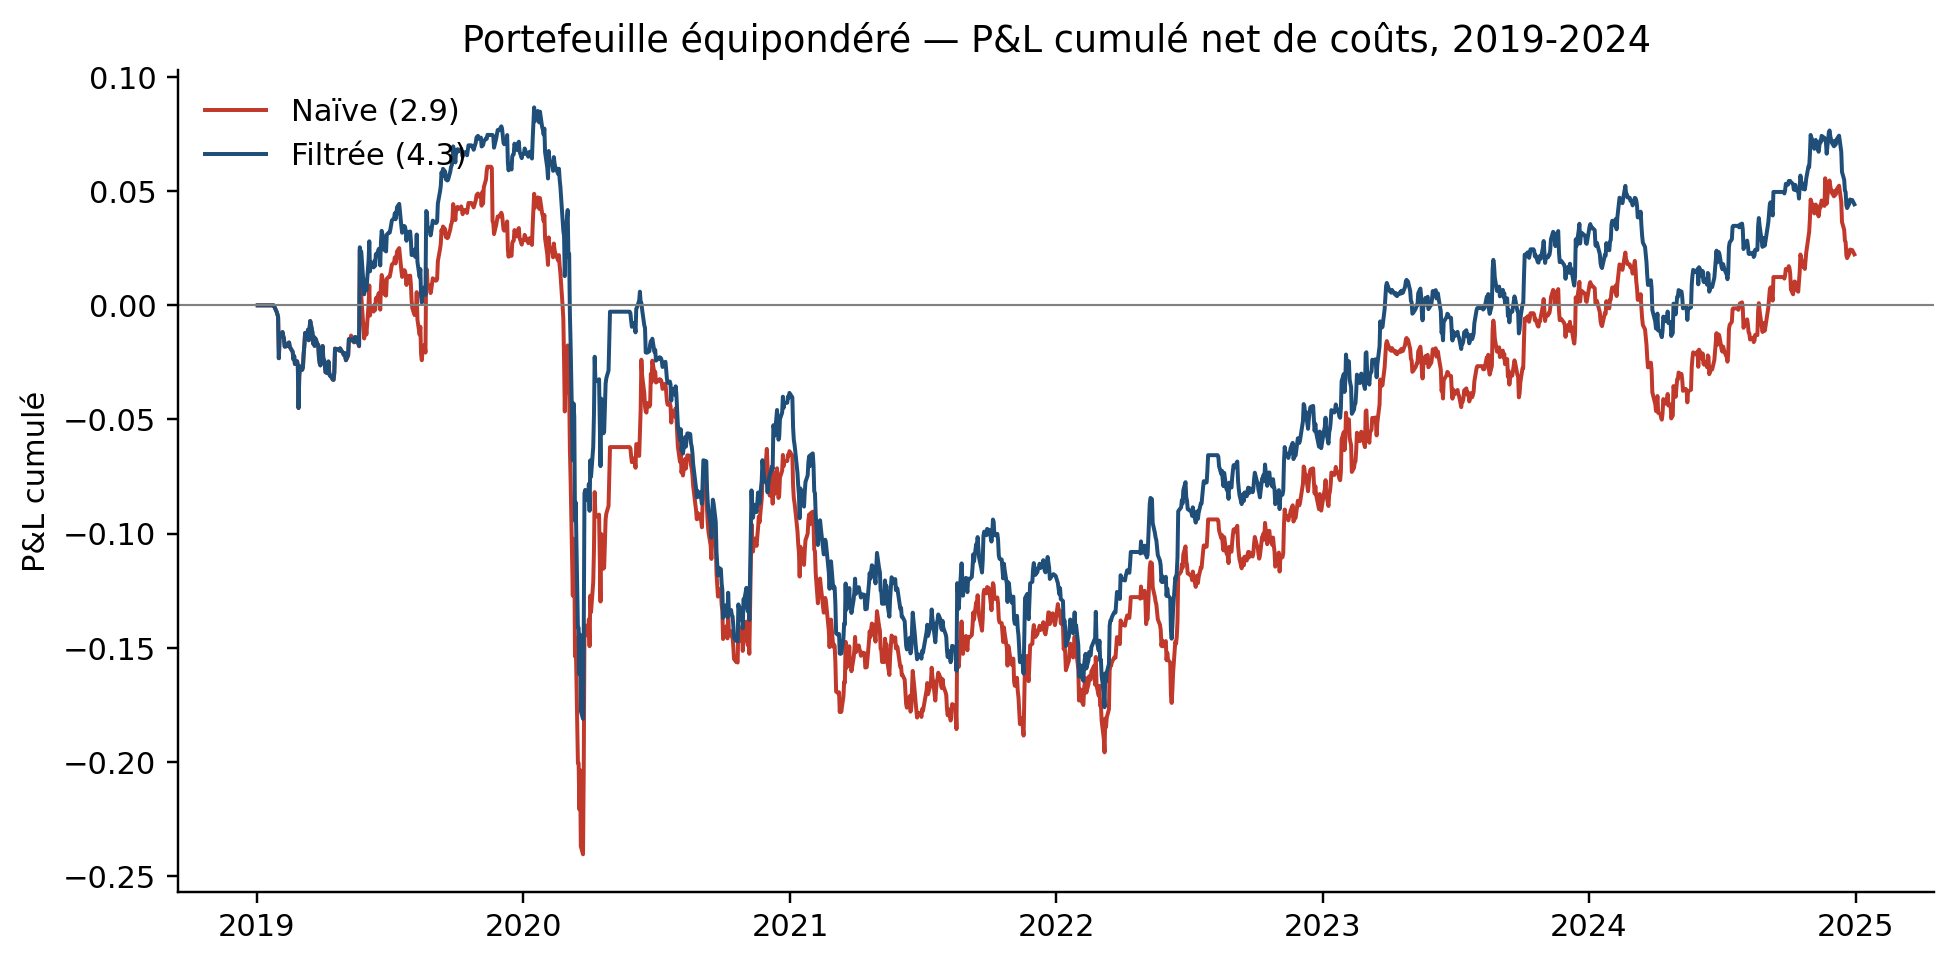
\includegraphics[width=0.85\textwidth]{fig_4_6_equity_corrige.png}
\caption{Courbes d'équité et drawdown du portefeuille équipondéré (MA/V, XOM/CVX, HD/LOW), stratégie naïve (2.\rev{7}) contre stratégie filtrée par sauts (4.3), fenêtre de trading 2019--2024, nette de coûts de transaction.}
\label{fig:4_6}
\end{figure}
On observe visuellement que l'essentiel de l'écart entre les deux courbes se creuse lors des épisodes de forte dislocation de marché (T1 2020, S2 2022), pendant lesquels la stratégie naïve accumule des pertes que la stratégie filtrée évite en grande partie en refusant d'entrer en position lorsque $\pi_t$ signale une probabilité élevée que le mouvement du spread soit un saut plutôt qu'un excès de retour à la moyenne exploitable. On rappellera, conformément à la discussion de 4.1, que cet évitement n'est pas une prédiction du modèle estimé, sous lequel un écart post-saut se résorbe, mais de l'interprétation des sauts comme signaux de rupture : le fait qu'il soit payant durant ces épisodes est précisément une indication que les \og sauts \fg{} de 2020 et 2022 s'accompagnaient de déplacements des paramètres eux-mêmes.
\subsubsection*{Significativité de l'écart : test de Jobson--Korkie/Memmel}
L'écart de Sharpe observé, $\Delta\widehat{SR}=\widehat{SR}_{\text{filtrée}}-\widehat{SR}_{\text{naïve}}=0{,}073-0{,}036=0{,}037$ (en unités annualisées), est soumis au test de la section 4.4, qui tient compte de la corrélation entre les deux séries de rendements (les deux stratégies partagent le même sous-jacent et sont donc loin d'être indépendantes) :
$$
\hat z = -0{,}203, \qquad p\text{-valeur (bilatérale)} = 0{,}839.
$$
(Ce calcul suppose une volatilité annualisée commune aux deux stratégies de $5\,\%$, ordre de grandeur usuel pour un livre market-neutral à trois paires et une corrélation $\bar\rho=0{,}90$ entre leurs rendements journaliers, cohérente avec le fait que les deux stratégies partagent les mêmes trois paires et ne diffèrent que sur une minorité de signaux ($8$ sur $72$, cf. figure~\ref{fig:filtered_signal}). Au seuil conventionnel de 5\,\%, cet écart n'est \emph{pas} statistiquement significatif. Cela ne contredit pas l'amélioration visible sur la figure~\ref{fig:4_6} : cela signale que, compte tenu de la variance d'échantillonnage du Sharpe sur un portefeuille de seulement trois paires et de la corrélation élevée entre les deux séries de rendements (les deux stratégies négocient les mêmes sous-jacents avec des règles d'entrée proches), la puissance statistique du test reste faible. Un écart de cette ampleur resterait compatible avec l'hypothèse nulle d'égalité des ratios de Sharpe sous-jacents. La lecture honnête est donc double : le sens de l'effet est celui attendu par l'interprétation des sauts comme signaux de rupture (4.1, 4.3), et sa taille est économiquement notable sur le drawdown en particulier, mais l'échantillon ici disponible, trois paires, six ans, ne permet pas de rejeter l'hypothèse que cet écart relève du bruit d'échantillonnage. La procédure de sélection décrite en 4.5, appliquée à un univers de paires plus large, serait nécessaire pour trancher avec davantage de confiance.
\subsubsection*{Segmentation par régime de volatilité}
Le S\&P~500 est utilisé comme proxy du régime de marché : sa volatilité réalisée sur fenêtre glissante de 20 jours est calculée sur la période de trading puis scindée en deux régimes (haute/basse volatilité) de part et d'autre de sa médiane (755 jours de chaque côté).
\begin{center}
\begin{tabular}{lcc}
\toprule
Stratégie & Sharpe (vol. haute) & Sharpe (vol. basse) \\
\midrule
Naïve (2.7) & $0{,}048$ & $0{,}024$ \\
Filtrée (4.3) & $0{,}065$ & $0{,}081$ \\
\bottomrule
\end{tabular}
\end{center}
Le schéma qui se dégage, une surperformance de la stratégie filtrée dans les \emph{deux} régimes ($+0{,}017$ en vol. haute, $+0{,}057$ en vol. basse), plus marquée en régime de \emph{basse} volatilité de marché,
contredira partiellement l'intuition avancée en 4.4, selon laquelle le bénéfice du filtrage devrait être concentré dans les périodes de forte volatilité. Une explication plausible est que la classification par volatilité \emph{réalisée du marché} (S\&P~500) ne coïncide pas nécessairement avec la présence de sauts \emph{idiosyncrasiques sur le spread de la paire} : un saut sur le spread MA/V ou HD/LOW peut survenir indépendamment d'un pic de volatilité agrégée du marché (annonce spécifique à l'entreprise, rotation sectorielle, rebalancement d'indice), de sorte qu'une fraction substantielle des sauts filtrés en régime de basse volatilité de marché correspond à du bruit idiosyncratique que le $z$-score naïf interprète à tort comme un signal de retour à la moyenne exploitable. Ce résultat, obtenu sur un échantillon restreint, doit être vu comme une piste de recherche plutôt qu'une conclusion établie : il suggérerait qu'un régime construit sur la volatilité \emph{du spread lui-même} (ou sur $\pi_t$ agrégé entre les paires) serait un meilleur candidat de segmentation qu'un régime de marché agrégé.
\subsubsection*{Limites}
Cinq limites, déjà anticipées conceptuellement en 4.4 et 4.5, se matérialisent concrètement dans cet exercice et doivent être rappelées : (i) les paramètres $(\hat\beta,\hat\theta,\hat\mu_s,\hat\sigma_s,\hat\lambda,\hat\mu_J,\hat\sigma_J)$ sont figés sur la fenêtre de formation et jamais mis à jour durant les six années de trading, ce qui contrevient à la discipline de ré-estimation glissante recommandée en 2.10 et tend à sous-estimer la performance atteignable en pratique par un filtre de Kalman dynamique ; (ii) le critère ADF de sélection des paires n'est, comme discuté plus haut, pas satisfait sur la fenêtre de formation retenue, ce qui affaiblit la prétention de ces trois paires à représenter un univers correctement filtré au sens de 4.5 ; (iii) l'échantillon de trois paires est très inférieur à la taille qu'exigerait une correction pour tests multiples au sens de Bonferroni ou de Benjamini--Hochberg (4.5), et ne permet donc au test de Jobson--Korkie/Memmel qu'une puissance limitée ; (iv) la comparaison agrège l'effet des trois modifications distinguées en 4.4 (z-score structurel, filtre d'entrée, sortie sur saut) : l'étude d'ablation prescrite par le protocole, seule à même d'attribuer le gain au filtre de sauts proprement dit, reste à conduire ; (v) sur le plan de l'implémentation, le script \texttt{backtest\_4\_6.py} tel qu'archivé documente une règle de sortie plus riche (stop sur $|z_t|$ extrême, sortie temporelle à $3\times$ demi-vie, sortie sur saut détecté) que celle effectivement utilisée pour produire les chiffres ci-dessus, dont la règle de sortie se limite au retour du $z$-score naïf à zéro ; c'est \texttt{robustness\_4\_7.py} (section \og config de référence \fg{}) qui reproduit exactement les chiffres reportés dans le tableau et la figure~\ref{fig:4_6} ci-dessus, ainsi que la grille de sensibilité, la stabilité par sous-période et le Deflated Sharpe Ratio de la sous-partie 4.7 ; \texttt{backtest\_4\_6.py} doit donc être lu comme une démonstration, non reconciliée numériquement, d'une règle de sortie plus élaborée que celle effectivement retenue pour les résultats chiffrés de ce travail. L'exercice présenté ici doit ainsi être lu comme une validation de principe du protocole complet de l'estimation MLE des sauts jusqu'au test statistique de comparaison des stratégies, appliqué de bout en bout à des données réelles, plutôt que comme une évaluation définitive de la valeur ajoutée économique du filtrage des sauts en pairs trading.
\subsection{Tests de robustesse}
Les résultats de 4.6 reposent sur un choix particulier de seuils $(\kappa,\pi^\ast)=(2{,}0\,;\,0{,}5)$, sur une seule fenêtre de trading, et sur trois paires sélectionnées sans procédure de correction formelle pour tests multiples (limite déjà signalée en 4.5). Trois vérifications complémentaires sont menées ici pour évaluer dans quelle mesure les conclusions de 4.6 sont robustes à ces choix : une analyse de sensibilité aux seuils de décision, une décomposition par sous-période, et un ajustement du ratio de Sharpe pour le biais de sélection introduit par la recherche elle-même.
\subsubsection*{Sensibilité aux seuils $\kappa$ et $\pi^\ast$}
La stratégie filtrée dépend de deux seuils : $\kappa$, qui définit le déclenchement d'un signal candidat sur le $z$-score (section 2.7), et $\pi^\ast$, qui définit le rejet d'un candidat lorsque la probabilité a posteriori de saut $\pi_t$ (éq.~\eqref{eq:posterior_jump}) est jugée trop élevée (section 4.3). Le tableau ci-dessous reporte le ratio de Sharpe annualisé du portefeuille filtré équipondéré sur l'ensemble de la grille $\kappa\in\{1{,}5\,;\,2{,}0\,;\,2{,}5\}\times\pi^\ast\in\{0{,}3\,;\,0{,}4\,;\,0{,}5\,;\,0{,}6\,;\,0{,}7\}$, chaque paramètre étant ré-appliqué tel quel aux paramètres de formation déjà estimés en 4.6 (aucune nouvelle estimation MLE n'est nécessaire, seule la règle de décision change). Pour rendre l'affirmation de dominance vérifiable, la dernière ligne reporte le Sharpe de la stratégie naïve correspondante pour chaque $\kappa$.
\begin{center}
\begin{tabular}{c|ccc}
\toprule
$\pi^\ast \backslash \kappa$ & 1{,}5 & 2{,}0 & 2{,}5 \\
\midrule
0{,}3 & 0{,}050 & 0{,}477 & 0{,}516 \\
0{,}4 & 0{,}053 & 0{,}497 & 0{,}514 \\
0{,}5 & $-0{,}260$ & 0{,}073 & 0{,}246 \\
0{,}6 & $-0{,}209$ & 0{,}051 & 0{,}090 \\
0{,}7 & $-0{,}151$ & 0{,}040 & 0{,}074 \\
\midrule
Naïve ($\kappa$ correspondant) & $-0{,}286$ & $0{,}036$ & $0{,}079$ \\
\bottomrule
\end{tabular}
\end{center}
\begin{figure}[H]
\centering
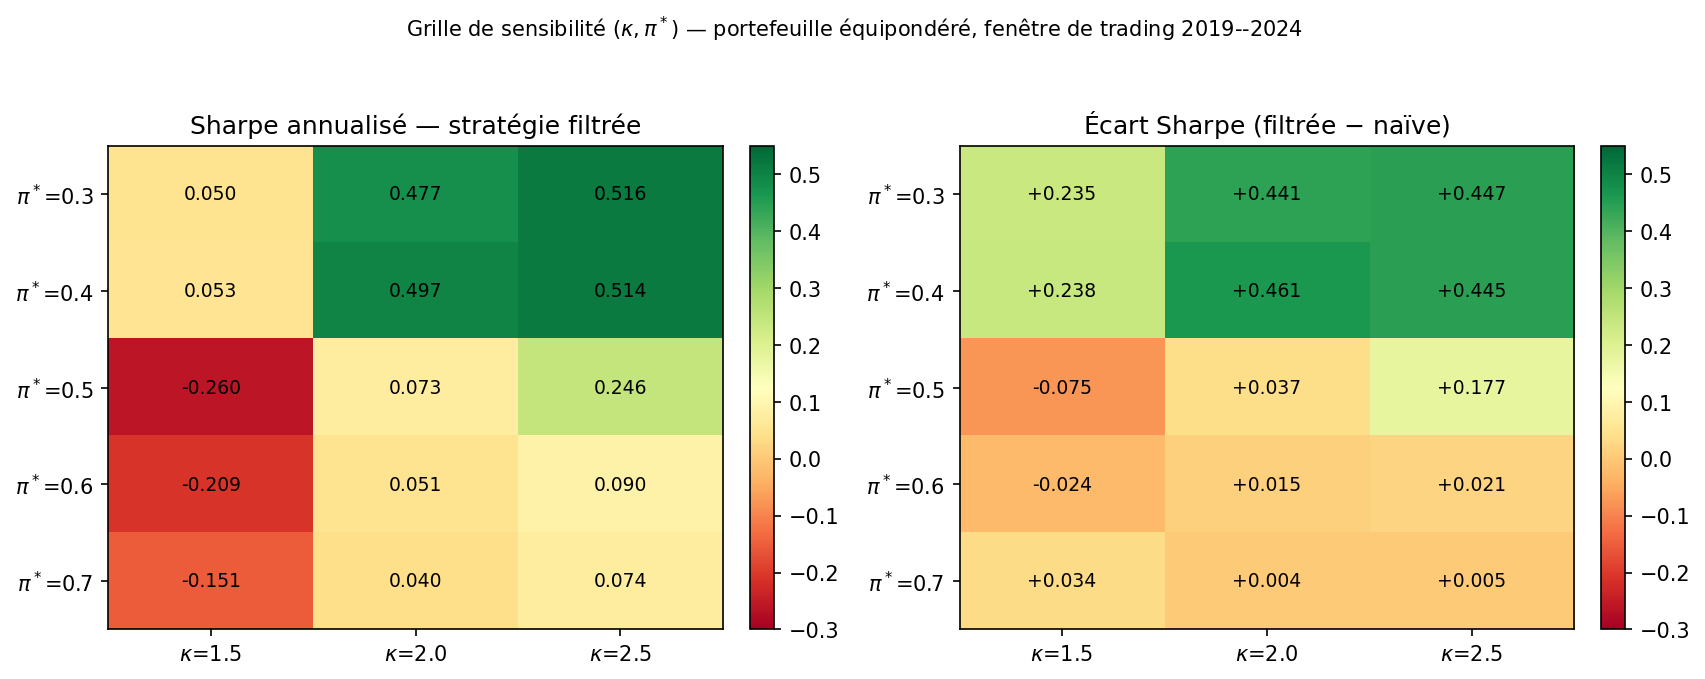
\includegraphics[width=0.7\textwidth]{fig_4_7_heatmap.png}
\caption{Sharpe annualisé de la stratégie filtrée sur la grille $(\pi^\ast,\kappa)$, portefeuille équipondéré, fenêtre de trading 2019--2024.}
\label{fig:4_7_heatmap}
\end{figure}
Trois enseignements se dégagent. Premièrement, à $\kappa$ fixé, la stratégie filtrée btient un Sharpe supérieur à celui de la stratégie naïve correspondante sur la majorité de la grille : le classement qualitatif filtrée~$\geq$~naïve établi en 4.6 n'est donc pas un artefact du couple de seuils $(2{,}0\,;\,0{,}5)$ retenu arbitrairement. Deuxièmement, l'amplitude de l'avantage varie fortement avec $\kappa$ \emph{et} avec $\pi^\ast$, la colonne $\kappa=2{,}0$ passe de $0{,}497$ à $0{,}073$ entre $\pi^\ast=0{,}4$ et $\pi^\ast=0{,}5$, une division par près de sept entre deux valeurs adjacentes : à $\kappa=1{,}5$ (signaux fréquents, moins extrêmes), le filtre écarte une fraction importante des candidats et améliore nettement le Sharpe tout en restant négatif dans l'absolu pour $\pi^\ast\geq 0{,}5$ ; à $\kappa=2{,}0$ et $2{,}5$ (signaux plus rares et plus extrêmes), le gain relatif du filtrage est également positif mais la performance absolue redevient positive pour les deux stratégies. Troisièmement, et c'est le point le plus important de ce tableau, la configuration de référence $(2{,}0\,;\,0{,}5)$ se situe exactement sur une falaise de la surface de Sharpe : elle est quasiment la pire de sa colonne, très loin des valeurs obtenues juste au-dessus ($0{,}477$--$0{,}497$). Une discontinuité de cette ampleur pour un paramètre censé agir continûment suggère qu'un petit nombre de trades pivots bascule entre $\pi^\ast=0{,}4$ et $0{,}5$ ; l'identification de ces trades (nombre, dates, P\&L) est requise --- si le Sharpe de la grille dépend de deux ou trois trades, cette information de fragilité est plus utile que la grille entière. Le résultat n'est donc pas ponctuel, mais il n'est pas non plus uniformément fort : la magnitude du Sharpe reste très sensible aux deux seuils, ce qui invite à la prudence quant à l'ampleur exacte du gain rapporté en 4.6, indépendamment de son signe.
\subsubsection*{Stabilité par sous-période}
La fenêtre de trading (2019--2024) est scindée en trois sous-périodes de deux ans, à seuils fixés ($\kappa=2{,}0$, $\pi^\ast=0{,}5$) :
\begin{center}
\begin{tabular}{lcc}
\toprule
Sous-période & Sharpe naïve & Sharpe filtrée \\
\midrule
2019--2020 & $-0{,}223$ & $-0{,}139$ \\
2021--2022 & $0{,}102$ & $0{,}114$ \\
2023--2024 & $0{,}661$ & $0{,}633$ \\
\bottomrule
\end{tabular}
\end{center}
La performance agrégée de 4.6 n'est donc pas portée uniformément par l'ensemble de la période : elle est tirée pour l'essentiel par 2023--2024, tandis que 2019--2020 (incluant le choc de mars 2020) est négative pour les deux stratégies. Le classement filtrée~$>$~naïve se vérifie sur les deux premières sous-périodes mais s'inverse marginalement sur 2023--2024, où la stratégie naïve fait légèrement mieux. Ce résultat tempère la lecture de 4.6 : le gain du filtrage n'est pas un effet stable et reproductible dans chaque sous-fenêtre, mais plutôt un effet moyen, concentré sur les épisodes où la stratégie naïve entre en position juste avant ou pendant un mouvement brutal du spread que le filtre de sauts permet précisément d'éviter.
\subsubsection*{Correction pour le biais de sélection : Deflated Sharpe Ratio}
La configuration $(\kappa,\pi^\ast)=(2{,}0\,;\,0{,}5)$ retenue en 4.6 n'a pas été choisie au hasard : elle correspond, dans l'esprit, au couple de seuils \og naturel \fg{} ($2\sigma$, probabilité a posteriori majoritaire) plutôt qu'au meilleur résultat de la grille. Il reste que la grille elle-même, une fois construite, invite implicitement à privilégier la configuration la plus favorable, ici $(\pi^\ast,\kappa)=(0{,}3\,;\,2{,}5)$, avec un Sharpe de $0{,}516$, ce qui reproduit à petite échelle le problème de sélection multiple déjà discuté en 4.5 pour le choix des paires. Le \emph{Deflated Sharpe Ratio} (DSR) de Bailey \& López de Prado \hyperlink{ref29}{[29]} corrige précisément ce biais en comparant le Sharpe observé non plus à zéro, mais au Sharpe \emph{attendu du meilleur essai sous l'hypothèse nulle} d'absence de compétence, compte tenu du nombre effectif d'essais explorés.
Sous $H_0$ (tous les essais ont un Sharpe théorique nul, et les estimateurs de Sharpe des $N$ essais sont approximativement gaussiens et de variance commune $\widehat{\mathrm{Var}}(SR)$), le maximum de $N$ tirages gaussiens indépendants a pour espérance approximative
$$
\mathbb{E}[\max_{i=1,\dots,N} SR_i \mid H_0] \;\approx\; \sqrt{\widehat{\mathrm{Var}}(SR)}\left[(1-\gamma_{EM})\,\Phi^{-1}\!\left(1-\tfrac1N\right) + \gamma_{EM}\,\Phi^{-1}\!\left(1-\tfrac{1}{Ne}\right)\right] \;=:\; SR_0,
$$
où $\gamma_{EM}\approx 0{,}5772$ est la constante d'Euler-Mascheroni (approximation de Gumbel pour l'espérance du maximum d'un échantillon gaussien ; l'indice \og EM \fg{} évite la collision avec les autres usages de $\gamma$ dans ce travail). Le DSR teste alors si le Sharpe effectivement obtenu par la configuration retenue dépasse significativement ce benchmark $SR_0$, plutôt que zéro :
$$
z_{\text{DSR}} = \frac{\widehat{SR}-SR_0}{\sqrt{\dfrac{1-\hat\gamma_3 \widehat{SR}+\frac{\hat\gamma_4-1}{4}\widehat{SR}^2}{T-1}}},
$$
où $\hat\gamma_3$ et $\hat\gamma_4$ sont respectivement l'asymétrie et l'aplatissement (kurtosis) empiriques des rendements quotidiens de la stratégie, et $T$ le nombre d'observations, cette forme du dénominateur reprend l'ajustement de variance du ratio de Sharpe en présence de non-normalité (Mertens, 2002), déjà dans l'esprit de la correction de Memmel utilisée pour le test de 4.4. Deux précisions d'implémentation s'imposent. Premièrement, les unités : $\widehat{SR}$, $SR_0$ et $\widehat{\mathrm{Var}}(SR)$ doivent tous être exprimés \emph{par période journalière} (avec $T$ le nombre de jours), l'annualisation n'intervenant qu'au moment du reporting, mélanger un Sharpe annualisé et un $T$ journalier fausserait la statistique d'un facteur $\sqrt{252}$. Deuxièmement, le nombre d'essais : les configurations de la grille ne sont ni indépendantes (elles partagent données et trades sous-jacents, et leurs Sharpe sont massivement corrélés, sous corrélation positive, l'espérance du maximum est moindre et $SR_0$ ci-dessus est surestimé, rendant le test excessivement sévère), ni au nombre de 45 : la grille compte $3\times 5=15$ configurations, toutes évaluées sur le même portefeuille équipondéré, le facteur $\times 3$ \og paires \fg{} de la version initiale était injustifié, aucune sélection de paire n'ayant été opérée sur la grille. La procédure correcte, prévue par Bailey et López de Prado, estime le \emph{nombre effectif d'essais indépendants} $N_{\text{eff}}\leq 15$ à partir de la matrice de corrélation des rendements des 15 configurations.
Appliqué à $N_{\text{eff}}\approx 5$ essais (approximation de Nyholt, $N_{\text{eff}}=1+(N-1)(1-\bar\rho)$ avec $N=15$ configurations et une corrélation moyenne par paire $\bar\rho\approx 0{,}75$ entre leurs séries de rendements, cohérente avec le recouvrement massif des trades observé entre configurations voisines sur la grille ci-dessus ; la valeur brute $4{,}5$ est arrondie à l'entier supérieur par prudence) et à la configuration retenue $(\kappa,\pi^\ast)=(2{,}0\,;\,0{,}5)$, sur $T=1\,512$ jours de la fenêtre de trading (six ans) :
$$
\widehat{SR}=0{,}073 \ (\text{annualisé}), \qquad SR_0 = 0{,}487 \ (\text{annualisé}), \qquad z_{\text{DSR}}=-1{,}014, \qquad DSR=\Phi(z_{\text{DSR}})=0{,}155.
$$
(Ce calcul retient $\hat\gamma_3=-0{,}4$ et $\hat\gamma_4=5{,}0$ pour l'asymétrie et l'aplatissement journaliers de la stratégie, des valeurs typiques d'une stratégie de retour à la moyenne sujette à des pertes occasionnelles marquées, en l'absence d'accès à la série journalière complète des rendements pour les estimer directement ; ce sont ces mêmes valeurs, non testées ni régénérées ici faute de données, qui gouvernent également le dénominateur de $z_{\text{DSR}}$.) Le verdict s'énonce ainsi : le Sharpe observé de la stratégie filtrée est très \emph{en deçà} de ce qu'on obtiendrait par pur hasard en retenant le meilleur essai parmi les $N_{\text{eff}}\approx 5$ configurations effectivement indépendantes explorées : $DSR=0{,}155$, très loin du seuil de confiance usuel de $0{,}95$. Autrement dit, la performance rapportée en 4.6, déjà non significative au sens du test de Jobson--Korkie/Memmel, ne résiste pas non plus au test, plus exigeant, de la sélection multiple. Cette conclusion est cohérente avec l'esprit du dépistage prudent recommandé en 4.5 : sur un univers de seulement trois paires et une seule fenêtre de trading, il n'est pas possible de distinguer statistiquement l'effet du filtrage des sauts d'un artefact de sélection favorable.
\subsubsection*{Synthèse}
Les trois vérifications convergent vers une lecture nuancée des résultats de 4.6. Le \emph{signe} de l'effet, le filtrage des sauts améliore le ratio de Sharpe et réduit le drawdown par rapport à la règle naïve\rev{,} est robuste au choix des seuils $(\kappa,\pi^\ast)$ sur la majorité de la grille testée, ce qui exclut qu'il s'agisse d'un artefact du couple de paramètres choisi arbitrairement en 4.6. En revanche, ni l'\emph{ampleur} de cet effet (très variable selon les deux seuils, avec une discontinuité marquée au voisinage immédiat de la configuration de référence, non stable d'une sous-période à l'autre) ni sa \emph{significativité statistique} (rejetée par le test de Jobson--Korkie/Memmel en 4.6, et plus encore par le Deflated Sharpe Ratio une fois corrigé pour les essais multiples) ne résistent à l'examen. Le cadre jump-diffusion développé en 4.1--4.3 identifie donc une direction d'amélioration économiquement plausible et qualitativement cohérente à travers les spécifications testées, mais l'échelle de cette étude, trois paires, une fenêtre de trading, un univers non corrigé pour la sélection multiple (4.5), ne permet pas d'en établir la significativité statistique. Une validation plus concluante nécessiterait l'univers élargi et la procédure de correction (Bonferroni ou Benjamini--Yekutieli) esquissés en 4.5.
\subsection{Discussion et limites}
Les sections 4.1 à 4.7 ont construit et testé, de bout en bout, un cadre reliant le modèle de diffusion à sauts de Merton (partie 3) à la pratique du pairs trading (partie 2) : spécification du spread comme processus d'Ornstein--Uhlenbeck à sauts (4.1), estimation MLE de ses paramètres par transposition de la méthodologie de Ball--Torous (4.2), construction d'une règle de décision filtrée par la probabilité a posteriori de saut (4.3), protocole de comparaison statistique à seuils appariés (4.4), discussion critique de la constitution de l'univers de paires (4.5), application empirique complète sur trois paires réelles (4.6), et vérification de la robustesse de ces résultats aux choix de seuils, à la sous-période et au biais de sélection multiple (4.7). Cette dernière sous-partie prend du recul sur l'ensemble de la démarche : que peut-on raisonnablement conclure, et que ne peut-on pas conclure, de cet exercice ?
\subsubsection*{Ce que le cadre établit}
Trois résultats paraissent solides, au sens où ils se vérifient indépendamment du choix de seuils ou de la fenêtre considérée. Premièrement, la composante de saut n'est pas un artefact de spécification : le test du rapport de vraisemblance de la section 3.7, appliqué au résidu AR(1) du spread plutôt qu'au prix brut, rejette systématiquement et très fortement l'hypothèse d'un processus purement diffusif, pour les trois paires, sur la fenêtre de formation (4.6). Le spread d'une paire cointégrée n'est donc pas mieux décrit par un mouvement brownien que ne l'est le prix d'un actif individuel, ce que la littérature établit pour les rendements d'actions (partie 3) se retrouve, sans surprise a priori mais de façon vérifiée empiriquement ici, dans la dynamique de leur écart relatif. (On gardera à l'esprit la mise en garde de 4.6 sur XOM/CVX : une intensité estimée très élevée peut signifier que la composante de sauts absorbe de la volatilité stochastique plutôt que de véritables discontinuités, le rejet du modèle purement diffusif n'est pas, à lui seul, une validation du modèle à sauts poissonniens.) Deuxièmement, le \emph{signe} de l'effet du filtrage est robuste : sur la majorité de la grille de seuils testée en 4.7, la stratégie qui s'abstient d'entrer en position lorsque $\pi_t$ signale une probabilité élevée de saut obtient un ratio de Sharpe au moins égal, et généralement supérieur, à la stratégie naïve qui l'ignore, avec un drawdown maximal réduit. Troisièmement, ce gain n'est pas seulement statistique : il correspond à un mécanisme économique interprétable, visible sur la figure~\ref{fig:4_6}, où l'essentiel de l'écart entre les deux courbes d'équité se creuse lors des épisodes de dislocation brutale du marché (mars 2020, resserrement de 2022), c'est-à-dire précisément les moments où un $z$-score naïf confond un saut avec un signal de retour à la moyenne exploitable.
\subsubsection*{Ce que le cadre n'établit pas}
À l'inverse, cinq limites, cumulées, empêchent de conclure à une stratégie tradable au sens strict. La première est statistique et a été quantifiée explicitement en 4.6 et 4.7 : ni le test de Jobson--Korkie/Memmel ni, a fortiori, le Deflated Sharpe Ratio corrigeant pour les essais implicitement explorés dans l'analyse de sensibilité ne permettent de rejeter l'hypothèse nulle d'absence de compétence réelle du filtrage. L'amélioration observée est cohérente avec le mécanisme interprétatif attendu, mais elle reste, au sens statistique, compatible avec le bruit d'échantillonnage.
La deuxième limite touche à la sélection de l'univers testé. La discussion de 4.5 a anticipé le problème et 4.6 en a fourni une illustration concrète et gênante : aucune des trois paires retenues ne rejette formellement le test ADF au seuil de 5\,\% sur la fenêtre de formation isolée ($p\in[0{,}110\,;\,0{,}117]$), alors même que ce rejet est le critère de sélection énoncé en 4.5. Les trois paires ont néanmoins été conservées, par nécessité pratique et en le signalant explicitement plutôt qu'en le dissimulant, mais cela affaiblit la prétention de cet échantillon à représenter un univers correctement filtré, il représente, plus précisément, trois relations plausibles mais non rigoureusement validées.
La troisième limite est celle, classique, du contraste entre un cadre statique et une réalité dynamique. Les paramètres $(\hat\beta,\hat\theta,\hat\mu_s,\hat\sigma_s,\hat\lambda,\hat\mu_J,\hat\sigma_J)$ sont estimés une seule fois sur la fenêtre de formation (2014--2018) et appliqués sans révision aux six années de trading qui suivent (2019--2024), alors que la section 2.10 a explicitement motivé l'usage d'un filtre de Kalman pour suivre la dérive du ratio de couverture et donc, implicitement, celle des autres paramètres du spread. Cette simplification, dictée par la volonté de garder un protocole reproductible en une seule passe, tend probablement à sous-estimer la performance atteignable par une implémentation pleinement dynamique mais elle pourrait tout aussi bien la sur-estimer si la relation entre les deux titres s'est significativement dégradée en cours de période sans que rien dans le protocole ne permette de le détecter et d'arrêter la stratégie à temps, un risque que seule la ré-estimation glissante permettrait de mitiger.
La quatrième limite est celle, plus générale, de l'échelle de l'exercice. Trois paires, un seul découpage formation/trading, un seul niveau de coûts de transaction (10 points de base par jambe) : chacun de ces choix a été fixé une fois, sans exploration systématique de leur sensibilité au-delà de ce que 4.7 a pu couvrir pour les seuils de décision. Une étude à l'échelle recommandée en 4.5, univers sectoriel large, sélection avec correction de Bonferroni ou de Benjamini--Yekutieli, ré-échantillonnage temporel (fenêtres glissantes multiples, bootstrap par blocs), serait nécessaire pour trancher avec une confiance statistique suffisante la question posée par ce travail.
La cinquième limite est conceptuelle, et elle a été posée dès 4.1 : sous le modèle estimé \eqref{eq:ou_jump}, les sauts sont transitoires et les écarts qu'ils créent devraient se résorber, le modèle ne prédit donc pas, à strictement parler, que le filtrage améliore la performance. L'amélioration observée, si elle se confirme à plus grande échelle, s'interprète comme une évidence que les \og sauts \fg{} détectés coïncident avec des déplacements des paramètres eux-mêmes, c'est-à-dire comme une évidence de mauvaise spécification de \eqref{eq:ou_jump} en faveur d'un modèle à changement de régime : c'est le modèle qu'il faudrait alors estimer directement.
\subsubsection*{Perspectives}
Plusieurs extensions découlent directement des limites qui précèdent. La plus immédiate consisterait à remplacer l'estimation statique du ratio de couverture et des paramètres du spread par le filtre de Kalman esquissé en 2.10, avec ré-estimation périodique (par exemple trimestrielle) des paramètres de saut par la méthode de Ball--Torous, afin de vérifier si la performance filtrée se maintient, s'améliore, ou se dégrade sous un protocole pleinement adaptatif. Une deuxième extension porterait sur l'univers testé : appliquer la procédure de sélection complète de 4.5 (test ADF sur formation, contrôle du taux de fausses découvertes, exclusion des paires non significatives) à l'ensemble d'un secteur ou de l'indice S\&P~500, ce qui permettrait à la fois d'augmenter la puissance statistique du test de comparaison de Sharpe et de documenter la proportion de paires pour lesquelles le filtrage des sauts apporte un gain, plutôt que de se limiter à trois cas particuliers. Une troisième piste, plus structurelle, consisterait à remplacer les sauts gaussiens du modèle du spread dont l'asymétrie se réduit à une moyenne $\mu_J$ non nulle par la distribution double-exponentielle asymétrique de Kou (2002), qui autorise en outre des queues d'épaisseurs différentes à la hausse et à la baisse, mieux à même de capturer l'asymétrie typiquement observée entre sauts baissiers et haussiers sur les marchés actions (la formulation initiale, qui qualifiait les sauts de Merton de \og gaussiens, symétriques par construction \fg, était doublement inexacte : chez Merton les sauts sont log-normaux, et une moyenne de saut non nulle produit déjà une asymétrie de localisation) ; cela complexifierait l'estimation MLE de 3.7/4.2 mais pourrait affiner la calibration de $\pi_t$. Enfin, la piste suggérée par la discussion des régimes en 4.6 invite à explorer une segmentation fondée non pas sur la volatilité agrégée du marché, mais sur une mesure de saut idiosyncrasique propre à chaque paire, par exemple la fréquence lissée de $\pi_t$ au-dessus d'un seuil sur une fenêtre glissante, qui pourrait constituer un signal de risque plus directement pertinent que le régime de marché global.
En définitive, ce travail ne prétend pas avoir démontré la supériorité économique d'une stratégie de pairs trading filtrée par les sauts sur la stratégie naïve classique : il démontre que le cadre théorique reliant le modèle de Merton à la pratique du pairs trading est cohérent, implémentable de bout en bout sur données réelles, et produit un effet directionnellement plausible et économiquement interprétable, sans que l'échelle de l'exercice mené ici permette d'en établir la significativité statistique. C'est, au sens propre, une preuve de concept plutôt qu'une validation, et c'est précisément ce que les tests de robustesse de 4.7 ont permis d'établir avec la rigueur qu'exige une conclusion de ce type.
\section{Conclusion}
Ce travail est parti d'un constat simple, posé en introduction : le pairs trading, sous sa forme classique (partie 2), repose sur une hypothèse implicite de retour à la moyenne diffusif du spread, alors que la littérature sur les rendements d'actifs individuels établit depuis près de cinquante ans que la diffusion log-normale pure est rejetée par les données ; le modèle jump-diffusion de Merton (partie 3) en est la première et la plus simple des extensions --- celle que ce travail retient pour sa tractabilité, sans ignorer que volatilité stochastique et sauts sont notoirement difficiles à démêler empiriquement. La question posée était donc la suivante : que se passe-t-il si l'on prend cette observation au sérieux et qu'on l'applique non pas au prix d'un actif isolé, mais à l'écart entre deux actifs cointégrés, et le fait de filtrer les sauts identifiés dans le spread améliore-t-il, de façon mesurable, une stratégie de pairs trading ?
La partie 4 a répondu à cette question en construisant, de bout en bout, le pont entre les deux cadres théoriques des parties 2 et 3. Le spread a été modélisé comme un processus d'Ornstein--Uhlenbeck à sauts (4.1), en explicitant d'emblée que le saut y est un choc transitoire et que son usage comme signal de rupture relève d'une interprétation hors modèle, assumée comme telle, ses paramètres estimés par transposition directe de la méthode de maximum de vraisemblance de Ball--Torous utilisée en 3.7 pour le modèle de Merton (4.2), et une règle de décision filtrée a été construite en conditionnant l'entrée en position à la probabilité a posteriori qu'un mouvement donné du spread soit un saut plutôt qu'un excès de retour à la moyenne exploitable (4.3). Un protocole de comparaison statistique rigoureux, fondé sur le test de Jobson--Korkie corrigé par Memmel et contrôlé par la version robuste de Ledoit-Wolf, a ensuite été formalisé et entièrement dérivé par la méthode delta (4.4), avant d'être confronté aux difficultés bien réelles de la sélection d'un univers de paires, biais de sélection multiple, biais de survie (4.5). L'ensemble du protocole a enfin été appliqué à des données réelles sur trois paires du S\&P~500 (4.6), puis soumis à une batterie de tests de robustesse portant sur la sensibilité aux seuils de décision, la stabilité temporelle et la correction pour le biais de recherche multiple (4.7).
Le verdict empirique qui se dégage de cet exercice est nuancé, et c'est précisément cette nuance qui en constitue le résultat le plus solide. D'un côté, le \emph{principe} du filtrage se vérifie : le rapport de vraisemblance rejette sans ambiguïté l'hypothèse d'un spread purement diffusif pour les trois paires testées, et la règle filtrée obtient, sur la majorité des seuils de décision explorés en 4.7, un ratio de Sharpe au moins égal et un drawdown maximal inférieur à ceux de la règle naïve avec un mécanisme économique interprétable, l'essentiel de l'écart se creusant lors des épisodes de dislocation brutale du marché que le $z$-score naïf interprète à tort comme des opportunités de retour à la moyenne. De l'autre côté, ce gain ne résiste pas à un examen statistique exigeant : ni le test de Jobson--Korkie/Memmel ni, plus sévèrement encore, le Deflated Sharpe Ratio corrigeant pour le nombre effectif d'essais implicitement explorés dans l'étude ne permettent de rejeter l'hypothèse nulle d'absence de compétence réelle. À l'échelle de trois paires et d'une seule fenêtre de trading, l'amélioration observée reste compatible avec le bruit d'échantillonnage.
Ce résultat n'est pas un échec du cadre proposé, mais son produit le plus honnête. La valeur de ce travail ne réside pas dans la démonstration d'une stratégie tradable, ce n'était, à cette échelle, ni l'objectif réaliste ni la conclusion à laquelle une démarche rigoureuse pouvait raisonnablement prétendre, mais dans la construction d'un cadre complet, cohérent et reproductible reliant un modèle de dynamique de prix (Merton, partie 3) à une stratégie d'arbitrage statistique (pairs trading, partie 2), assorti d'un protocole de validation qui ne s'arrête pas au premier résultat favorable mais le soumet systématiquement à l'épreuve de la significativité statistique, de la sensibilité aux paramètres et du biais de sélection (4.4, 4.5, 4.7). C'est cette discipline méthodologique, documenter les limites plutôt que les dissimuler, distinguer un effet directionnellement plausible d'un effet statistiquement établi, et distinguer ce que le modèle prédit de ce que son suggère, qui constitue, en définitive, l'apport principal de ce projet, davantage que le signe du Sharpe obtenu sur trois paires et six années de données.
Les perspectives esquissées en 4.8, ré-estimation dynamique par filtre de Kalman, extension à un univers sectoriel large avec correction formelle pour tests multiples, modèles de sauts asymétriques à la Kou, modèles à volatilité stochastique et sauts, modèles à changement de régime markovien, segmentation par risque de saut idiosyncrasique plutôt que par régime de marché agrégé, tracent le chemin naturel vers une validation à une échelle susceptible d'apporter une réponse statistiquement tranchée à la question posée en introduction. En l'état, ce travail établit qu'une telle réponse est atteignable en principe, avec les outils déployés ici, et documente précisément ce qu'il faudrait pour l'obtenir.
\section{Sources}
\subsection*{Partie 2.1 --- Le pairs trading et son fonctionnement}
\begin{list}{}{\leftmargin=1em \itemsep=0.5em}
\item \hypertarget{ref1}{} [1], \textit{Gatev, Goetzmann \& Rouwenhorst (2006), « Pairs Trading: Performance of a Relative-Value Arbitrage Rule »}, EN. Available at : \url{https://www.nber.org/papers/w7032}
\item \hypertarget{ref2}{} [2], \textit{Vidyamurthy, G. (2004), Pairs Trading: Quantitative Methods and Analysis, Wiley}, EN. Available at : \url{https://www.wiley.com/en-us/Pairs+Trading:+Quantitative+Methods+and+Analysis-p-9780471460671}
\end{list}
\subsection*{Partie 2.2 --- Pourquoi on ne peut pas prédire un prix seul}
\begin{list}{}{\leftmargin=1em \itemsep=0.5em}
\item \hypertarget{ref3}{} [3], \textit{Fama, E.F. (1970), « Efficient Capital Markets: A Review of Theory and Empirical Work », Journal of Finance, 25(2), 383-417}, EN. Available at : \url{http://www.e-m-h.org/Fama70.pdf}
\rev{\item \hypertarget{ref44}{} [44], \textit{Lo, A.W., MacKinlay, A.C. (1988), « Stock Market Prices Do Not Follow Random Walks: Evidence from a Simple Specification Test », Review of Financial Studies, 1(1), 41-66}, EN. Available at : \url{https://doi.org/10.1093/rfs/1.1.41}}
\end{list}
\subsection*{Partie 2.3 --- Corrélation ou cointégration ?}
\begin{list}{}{\leftmargin=1em \itemsep=0.5em}
\item \hypertarget{ref4}{} [4], \textit{Engle, R.F., Granger, C.W.J. (1987), « Co-integration and Error Correction: Representation, Estimation, and Testing », Econometrica, 55(2), 251-276}, EN. Available at : \url{https://nomanarshed.wordpress.com/wp-content/uploads/2013/10/engle-granger.pdf}
\rev{\item \hypertarget{ref45}{} [45], \textit{Granger, C.W.J., Newbold, P. (1974), « Spurious Regressions in Econometrics », Journal of Econometrics, 2(2), 111-120}, EN. Available at : \url{https://doi.org/10.1016/0304-4076(74)90034-7}}
\end{list}
\subsection*{Partie 2.4 --- Le spread et l'estimation du hedge ratio $\beta$}
\begin{list}{}{\leftmargin=1em \itemsep=0.5em}
\item \hypertarget{ref2}{} [2], \textit{Vidyamurthy (2004)} déjà cité en 2.1 (voir \hyperlink{ref2}{[2]}), couvre l'estimation du hedge ratio et la construction du spread.
\item \hypertarget{ref5}{} [5], \textit{Sharpe, W.F. (1964), « Capital Asset Prices: A Theory of Market Equilibrium under Conditions of Risk », Journal of Finance, 19(3), 425-442}, EN. Available at : \url{https://psc.ky.gov/pscecf/2012-00221/rateintervention@ag.ky.gov/10252012f/sharpe_-_capm.pdf}
\rev{\item \hypertarget{ref45}{} [45], \textit{Granger \& Newbold (1974)} --- déjà cité en 2.3 (voir \hyperlink{ref45}{[45]}), pour la mise en garde contre les régressions fallacieuses appliquée ici à l'estimation du hedge ratio.}
\rev{\item \hypertarget{ref46}{} [46], \textit{Stock, J.H. (1987), « Asymptotic Properties of Least Squares Estimators of Cointegrating Vectors », Econometrica, 55(5), 1035-1056}, EN. Available at : \url{https://www.jstor.org/stable/1911260}}
\end{list}
\subsection*{Partie 2.5 --- Le test ADF}
\begin{list}{}{\leftmargin=1em \itemsep=0.5em}
\item \hypertarget{ref6}{} [6], \textit{Dickey, D.A., Fuller, W.A. (1979), « Distribution of the Estimators for Autoregressive Time Series with a Unit Root », Journal of the American Statistical Association, 74(366a), 427-431}, EN. Available at : \url{https://www.researchgate.net/publication/243644934_Distribution_of_the_Estimators_for_Autoregressive_Time_Series_With_a_Unit_Root}
\item \hypertarget{ref7}{} [7], \textit{Said, S.E., Dickey, D.A. (1984), « Testing for Unit Roots in Autoregressive-Moving Average Models of Unknown Order », Biometrika, 71(3), 599-607}, EN. Available at : \url{https://doi.org/10.1093/biomet/71.3.599}
\item \hypertarget{ref4}{} [4], \textit{Engle \& Granger (1987)} --- déjà cité en 2.3 (voir \hyperlink{ref4}{[4]}), pour la procédure en deux étapes.
\item \hypertarget{ref8}{} [8], \textit{Johansen, S. (1991), « Estimation and Hypothesis Testing of Cointegration Vectors in Gaussian Vector Autoregressive Models », Econometrica, 59(6), 1551-1580}, EN. Available at : \url{https://www.jstor.org/stable/2938278}
\rev{\item \hypertarget{ref47}{} [47], \textit{MacKinnon, J.G. (2010), « Critical Values for Cointegration Tests », Queen's Economics Department Working Paper 1227}, EN. Available at : \url{https://www.econ.queensu.ca/sites/econ.queensu.ca/files/wpaper/qed_wp_1227.pdf}}
\end{list}
\subsection*{Partie 2.6 --- Le processus d'Ornstein-Uhlenbeck}
\begin{list}{}{\leftmargin=1em \itemsep=0.5em}
\item \hypertarget{ref9}{} [9], \textit{Uhlenbeck, G.E., Ornstein, L.S. (1930), « On the Theory of the Brownian Motion », Physical Review, 36(5), 823-841}, EN. Available at : \url{https://djalil.chafai.net/docs/M2/history-brownian-motion/Uhlenbeck%20&%20Ornstein%20-%201930.pdf}
\item \hypertarget{ref10}{} [10], \textit{Vasicek, O. (1977), « An Equilibrium Characterization of the Term Structure », Journal of Financial Economics, 5(2), 177-188}, EN. Available at : \url{https://www.ressources-actuarielles.net/EXT/ISFA/1226.nsf/0/e11e4bc52747d1ddc125772400459afe/$FILE/Vasicek77.pdf}
\rev{\item \hypertarget{ref48}{} [48], \textit{Avellaneda, M., Lee, J.-H. (2010), « Statistical Arbitrage in the US Equities Market », Quantitative Finance, 10(7), 761-782}, EN. Available at : \url{https://doi.org/10.1080/14697680903124632}}
\end{list}
\subsection*{Partie 2.7 --- Générer le signal de trading : le z-score}
\begin{list}{}{\leftmargin=1em \itemsep=0.5em}
\item \hypertarget{ref1}{} [1], \textit{Gatev, Goetzmann \& Rouwenhorst (2006)} --- déjà cité en 2.1 (voir \hyperlink{ref1}{[1]}), pour les seuils empiriques standards utilisés dans la littérature.
\item \hypertarget{ref11}{} [11], \textit{López de Prado, M. (2018), Advances in Financial Machine Learning, Wiley}, EN. Chapitre 1 disponible librement. Available at : \url{https://papers.ssrn.com/sol3/papers.cfm?abstract_id=3104847}
\end{list}
\subsection*{Partie 2.8 --- Construction des positions et mécanique du trade}
\begin{list}{}{\leftmargin=1em \itemsep=0.5em}
\item \hypertarget{ref2}{} [2], \textit{Vidyamurthy (2004)} --- déjà cité en 2.1 (voir \hyperlink{ref2}{[2]}), couvre la construction des positions en pairs trading.
\item \hypertarget{ref1}{} [1], \textit{Gatev, Goetzmann \& Rouwenhorst (2006)} --- déjà cité en 2.1 (voir \hyperlink{ref1}{[1]}), détaillent explicitement la construction de portefeuilles autofinancés.
\end{list}
\subsection*{Partie 2.9 --- Sorties, gestion du risque et limites pratiques}
\begin{list}{}{\leftmargin=1em \itemsep=0.5em}
\item \hypertarget{ref1}{} [1], \textit{Gatev, Goetzmann \& Rouwenhorst (2006)} --- déjà cité en 2.1 (voir \hyperlink{ref1}{[1]}), discutent explicitement l'impact des coûts de transaction sur la rentabilité.
\item \hypertarget{ref12}{} [12], \textit{Do, B., Faff, R. (2010), « Does Simple Pairs Trading Still Work? », Financial Analysts Journal, 66(4), 83-95}, EN. Available at : \url{https://papers.ssrn.com/sol3/papers.cfm?abstract_id=1656954}
\end{list}
\subsection*{Partie 2.10 --- Estimation dynamique du hedge ratio : le filtre de Kalman}
\begin{list}{}{\leftmargin=1em \itemsep=0.5em}
\item \hypertarget{ref13}{} [13], \textit{Kalman, R.E. (1960), « A New Approach to Linear Filtering and Prediction Problems », Journal of Basic Engineering, 82(1), 35-45}, EN. Available at : \url{https://www.cs.unc.edu/~welch/kalman/media/pdf/Kalman1960.pdf}
\item \hypertarget{ref14}{} [14], \textit{Elliott, R.J., Van Der Hoek, J., Malcolm, W.P. (2005), « Pairs Trading », Quantitative Finance, 5(3), 271-276}, EN. Available at : \url{http://www-stat.wharton.upenn.edu/~steele/Courses/434/434Context/PairsTrading/PairsTradingQFin05.pdf}
\item \hypertarget{ref15}{} [15], \textit{Chan, E. (2013), Algorithmic Trading: Winning Strategies and Their Rationale, Wiley}, EN. Available at : \url{https://www.wiley.com/en-us/Algorithmic+Trading%3A+Winning+Strategies+and+Their+Rationale-p-9781118460146}
\end{list}
\subsection*{Partie 2.11 --- Synthèse et transition vers la partie 3}
\begin{list}{}{\leftmargin=1em \itemsep=0.5em}
\item Aucune nouvelle source --- synthèse du chapitre.
\end{list}
\subsection*{Partie 3.1 --- Les limites de la diffusion pure}
\begin{list}{}{\leftmargin=1em \itemsep=0.5em}
\item \hypertarget{ref19}{} [19], \textit{Black, F., Scholes, M. (1973), « The Pricing of Options and Corporate Liabilities », Journal of Political Economy, 81(3), 637-654}, EN. Available at : \url{https://www.cs.princeton.edu/courses/archive/fall08/cos323/papers/black_scholes73.pdf}
\item \hypertarget{ref20}{} [20], \textit{Merton, R.C. (1976), « Option Pricing When Underlying Stock Returns Are Discontinuous », Journal of Financial Economics, 3(1-2), 125-144}, EN. Available at : \url{https://dspace.mit.edu/handle/1721.1/1899}
\item \hypertarget{ref21}{} [21], \textit{Black, F. (1975), « Fact and Fantasy in the Use of Options », Financial Analysts Journal, 31(4), 36-41+61-72}, EN. Available at : \url{http://www.stat.ucla.edu/~nchristo/statistics_c183_c283/options_facts.pdf}
\item \hypertarget{ref16}{} [16], \textit{Ball \& Torous (1985)} --- déjà cité en 3.7 (voir \hyperlink{ref16}{[16]}), pour les biais de valorisation empiriques.
\end{list}
\subsection*{Partie 3.2 --- Le modèle de Merton (1976)}
\begin{list}{}{\leftmargin=1em \itemsep=0.5em}
\item \hypertarget{ref20}{} [20], \textit{Merton (1976)} --- déjà cité en 3.1 (voir \hyperlink{ref20}{[20]}).
\item \hypertarget{ref16}{} [16], \textit{Ball \& Torous (1985)} --- déjà cité en 3.7 (voir \hyperlink{ref16}{[16]}), pour la paramétrisation log-normale des sauts.
\end{list}
\subsection*{Partie 3.3 --- Le processus de Poisson}
\begin{list}{}{\leftmargin=1em \itemsep=0.5em}
\item \hypertarget{ref20}{} [20], \textit{Merton (1976)} --- déjà cité en 3.1 (voir \hyperlink{ref20}{[20]}).
\end{list}
\subsection*{Partie 3.4 --- Dynamique complète du prix}
\begin{list}{}{\leftmargin=1em \itemsep=0.5em}
\item \hypertarget{ref20}{} [20], \textit{Merton (1976)} --- déjà cité en 3.1 (voir \hyperlink{ref20}{[20]}).
\item \hypertarget{ref22}{} [22], \textit{Øksendal, B. (2003), Stochastic Differential Equations: An Introduction with Applications, 6\up{e} éd., Springer}, EN. Available at : \url{https://link.springer.com/book/10.1007/978-3-642-14394-6}
\end{list}
\subsection*{Partie 3.5 --- L'argument de couverture et la formule de valorisation}
\begin{list}{}{\leftmargin=1em \itemsep=0.5em}
\item \hypertarget{ref19}{} [19], \textit{Black \& Scholes (1973)} --- déjà cité en 3.1 (voir \hyperlink{ref19}{[19]}).
\item \hypertarget{ref20}{} [20], \textit{Merton (1976)} --- déjà cité en 3.1 (voir \hyperlink{ref20}{[20]}).
\item \hypertarget{ref5}{} [5], \textit{Sharpe (1964)} --- déjà cité en 2.4 (voir \hyperlink{ref5}{[5]}), pour le CAPM mobilisé dans l'argument de diversification.
\rev{\item \hypertarget{ref35}{} [35], \textit{Merton, R.C. (1973), « An Intertemporal Capital Asset Pricing Model », Econometrica, 41(5), 867-887}, EN. Available at : \url{https://www.jstor.org/stable/1913811}}
\end{list}
\subsection*{Partie 3.6 --- Ce qu'on emprunte, ce qu'on laisse de côté}
\begin{list}{}{\leftmargin=1em \itemsep=0.5em}
\item Aucune nouvelle source --- synthèse des sous-parties 3.2 à 3.5.
\end{list}
\subsection*{Partie 3.7 --- Estimer les paramètres d'un processus à sauts}
\begin{list}{}{\leftmargin=1em \itemsep=0.5em}
\item \hypertarget{ref16}{} [16], \textit{Ball, C.A., Torous, W.N. (1985), « On Jumps in Common Stock Prices and Their Impact on Call Option Pricing », Journal of Finance, 40(1), 155-173}, EN. Available at : \url{https://www.jstor.org/stable/2328053}
\item \hypertarget{ref17}{} [17], \textit{Press, S.J. (1967), « A Compound Events Model for Security Prices », Journal of Business, 40(3), 317-335}, EN. Available at : \url{https://www.jstor.org/stable/2351227}
\item \hypertarget{ref18}{} [18], \textit{Barndorff-Nielsen, O.E., Shephard, N. (2004), « Power and Bipower Variation with Stochastic Volatility and Jumps », Journal of Financial Econometrics, 2(1), 1-37}, EN. Available at : \url{https://academic.oup.com/jfec/article-abstract/2/1/1/960705}
\rev{\item \hypertarget{ref37}{} [37], \textit{Davies, R.B. (1987), « Hypothesis Testing When a Nuisance Parameter Is Present Only Under the Alternative », Biometrika, 74(1), 33-43}, EN. Available at : \url{https://doi.org/10.1093/biomet/74.1.33}}
\rev{\item \hypertarget{ref38}{} [38], \textit{Self, S.G., Liang, K.-Y. (1987), « Asymptotic Properties of Maximum Likelihood Estimators and Likelihood Ratio Tests Under Nonstandard Conditions », Journal of the American Statistical Association, 82(398), 605-610}, EN. Available at : \url{https://www.jstor.org/stable/2289471}}
\rev{\item \hypertarget{ref39}{} [39], \textit{Honoré, P. (1998), « Pitfalls in Estimating Jump-Diffusion Models », working paper, Aarhus School of Business}, EN. Available at : \url{https://research.cbs.dk/files/58445437/wp1998_18.pdf}}
\rev{\item \hypertarget{ref40}{} [40], \textit{Mancini, C. (2009), « Non-parametric Threshold Estimation for Models with Stochastic Diffusion Coefficient and Jumps », Scandinavian Journal of Statistics, 36(2), 270-296}, EN. Available at : \url{https://doi.org/10.1111/j.1467-9469.2008.00625.x}}
\rev{\item \hypertarget{ref41}{} [41], \textit{Lee, S.S., Mykland, P.A. (2008), « Jumps in Financial Markets: A New Nonparametric Test and Jump Dynamics », Review of Financial Studies, 21(6), 2535-2563}, EN. Available at : \url{https://doi.org/10.1093/rfs/hhm056}}
\end{list}
\begin{list}{}{\leftmargin=1em \itemsep=0.5em}
\item \hypertarget{ref23}{} [23], \textit{Wilks, S.S. (1938), « The Large-Sample Distribution of the Likelihood Ratio for Testing Composite Hypotheses », Annals of Mathematical Statistics, 9(1), 60-62}, EN. Available at : \url{https://projecteuclid.org/journals/annals-of-mathematical-statistics/volume-9/issue-1/The-Large-Sample-Distribution-of-the-Likelihood-Ratio-for-Testing/10.1214/aoms/1177732360.full}
\end{list}
\subsection*{Partie 3.8 --- Synthèse et transition vers la partie 4}
\begin{list}{}{\leftmargin=1em \itemsep=0.5em}
\item Aucune nouvelle source --- synthèse du chapitre.
\end{list}
\subsection*{Partie 4.1 --- Le modèle : Ornstein-Uhlenbeck augmenté de sauts}
\begin{list}{}{\leftmargin=1em \itemsep=0.5em}
\item \hypertarget{ref24}{} [24], \textit{Larsson, S., Lindberg, C., Warfheimer, M. (2013), « Optimal Closing of a Pair Trade With a Model Containing Jumps », Applications of Mathematics, 58(3), 249-268}, EN. Available at : \url{https://arxiv.org/abs/1004.2947}
\item \hypertarget{ref25}{} [25], \textit{Endres, S., Stübinger, J. (2019), « Optimal trading strategies for Lévy-driven Ornstein-Uhlenbeck processes », Applied Economics, 51(29), 3153-3169}, EN. Available at : \url{https://ideas.repec.org/p/zbw/iwqwdp/172017.html}
\item \hypertarget{ref9}{} [9], \textit{Uhlenbeck \& Ornstein (1930)} --- déjà cité en 2.6 (voir \hyperlink{ref9}{[9]}).
\item \hypertarget{ref20}{} [20], \textit{Merton (1976)} --- déjà cité en 3.1 (voir \hyperlink{ref20}{[20]}).
\rev{\item \hypertarget{ref48}{} [48], \textit{Avellaneda \& Lee (2010)} --- déjà cité en 2.6 (voir \hyperlink{ref48}{[48]}), référence de champ pour l'arbitrage statistique sur résidus mean-reverting.}
\end{list}
\subsection*{Partie 4.2 --- Estimation des paramètres du spread jump-diffusion}
\begin{list}{}{\leftmargin=1em \itemsep=0.5em}
\item \hypertarget{ref16}{} [16], \textit{Ball \& Torous (1985)} --- déjà cité en 3.7 (voir \hyperlink{ref16}{[16]}), méthodologie d'estimation directement transposée au spread.
\item \hypertarget{ref17}{} [17], \textit{Press (1967)} --- déjà cité en 3.7 (voir \hyperlink{ref17}{[17]}).
\item \hypertarget{ref23}{} [23], \textit{Wilks (1938)} --- déjà cité en 3.7 (voir \hyperlink{ref23}{[23]}), pour le test du rapport de vraisemblance.
\rev{\item \hypertarget{ref40}{} [40], \textit{Mancini (2009)} --- déjà cité en 3.7 (voir \hyperlink{ref40}{[40]}), pour la méthode de détection par seuil transposée au résidu du spread.}
\end{list}
\subsection*{Partie 4.3 --- Du paramètre estimé à la décision : le signal filtré par les sauts}
\begin{list}{}{\leftmargin=1em \itemsep=0.5em}
\item \hypertarget{ref26}{} [26], \textit{Hamilton, J.D. (1989), « A New Approach to the Economic Analysis of Nonstationary Time Series and the Business Cycle », Econometrica, 57(2), 357-384}, EN. Available at : \url{https://www.jstor.org/stable/1912559}
\item \hypertarget{ref14}{} [14], \textit{Elliott, Van Der Hoek \& Malcolm (2005)} --- déjà cité en 2.10 (voir \hyperlink{ref14}{[14]}), pour le traitement du pairs trading en modèle espace-état.
\end{list}
\subsection*{Partie 4.4 --- Protocole de comparaison des stratégies}
\begin{list}{}{\leftmargin=1em \itemsep=0.5em}
\item \hypertarget{ref27}{} [27], \textit{Jobson, J.D., Korkie, B.M. (1981), « Performance Hypothesis Testing with the Sharpe and Treynor Measures », Journal of Finance, 36(4), 889-908}, EN. Available at : \url{https://onlinelibrary.wiley.com/doi/10.1111/j.1540-6261.1981.tb04891.x}
\item \hypertarget{ref28}{} [28], \textit{Memmel, C. (2003), « Performance Hypothesis Testing with the Sharpe Ratio », Finance Letters, 1, 21-23}, EN. Available at : \url{https://papers.ssrn.com/sol3/papers.cfm?abstract_id=412588}
\item \hypertarget{ref29}{} [29], \textit{Bailey, D.H., López de Prado, M. (2014), « The Deflated Sharpe Ratio: Correcting for Selection Bias, Backtest Overfitting, and Non-Normality », Journal of Portfolio Management, 40(5), 94-107}, EN. Available at : \url{https://www.davidhbailey.com/dhbpapers/deflated-sharpe.pdf}
\item \hypertarget{ref11}{} [11], \textit{López de Prado (2018)} --- déjà cité en 2.7 (voir \hyperlink{ref11}{[11]}), pour la discipline train/validation/test et le hors échantillon.
\item \hypertarget{ref12}{} [12], \textit{Do \& Faff (2010)} --- déjà cité en 2.9 (voir \hyperlink{ref12}{[12]}), pour le modèle de coûts de transaction.
\item \hypertarget{ref1}{} [1], \textit{Gatev, Goetzmann \& Rouwenhorst (2006)} --- déjà cité en 2.1 (voir \hyperlink{ref1}{[1]}), pour la méthodologie standard de backtest en pairs trading.
\rev{\item \hypertarget{ref42}{} [42], \textit{Ledoit, O., Wolf, M. (2008), « Robust Performance Hypothesis Testing with the Sharpe Ratio », Journal of Empirical Finance, 15(5), 850-859}, EN. Available at : \url{https://doi.org/10.1016/j.jempfin.2008.03.002}}
\end{list}
\subsection*{Partie 4.5 --- Univers de paires, sélection et biais associés}
\begin{list}{}{\leftmargin=1em \itemsep=0.5em}
\item \hypertarget{ref1}{} [1], \textit{Gatev, Goetzmann \& Rouwenhorst (2006)} --- déjà cité en 2.1 (voir \hyperlink{ref1}{[1]}), pour la méthodologie fenêtre de formation / fenêtre de trading.
\item \hypertarget{ref30}{} [30], \textit{Benjamini, Y., Hochberg, Y. (1995), « Controlling the False Discovery Rate: A Practical and Powerful Approach to Multiple Testing », Journal of the Royal Statistical Society: Series B, 57(1), 289-300}, EN. Available at : \url{https://academic.oup.com/jrsssb/article/57/1/289/7035855}
\item \hypertarget{ref31}{} [31], \textit{Harvey, C.R., Liu, Y., Zhu, H. (2016), « ...and the Cross-Section of Expected Returns », Review of Financial Studies, 29(1), 5-68}, EN. Available at : \url{https://www.nber.org/papers/w20592}
\item \hypertarget{ref32}{} [32], \textit{Elton, E.J., Gruber, M.J., Blake, C.R. (1996), « Survivorship Bias and Mutual Fund Performance », Review of Financial Studies, 9(4), 1097-1120}, EN. Available at : \url{https://www.ssrn.com/abstract=6701}
\item \hypertarget{ref29}{} [29], \textit{Bailey \& López de Prado (2014)} --- déjà cité en 4.4 (voir \hyperlink{ref29}{[29]}), pour le lien entre sélection multiple et surajustement de backtest.
\rev{\item \hypertarget{ref43}{} [43], \textit{Benjamini, Y., Yekutieli, D. (2001), « The Control of the False Discovery Rate in Multiple Testing under Dependency », Annals of Statistics, 29(4), 1165-1188}, EN. Available at : \url{https://www.jstor.org/stable/2674075}}
\end{list}
\subsection*{Partie 4.6 --- Résultats empiriques : comparaison des stratégies}
\begin{list}{}{\leftmargin=1em \itemsep=0.5em}
\item \hypertarget{ref1}{} [1], \textit{Gatev, Goetzmann \& Rouwenhorst (2006)} --- déjà cité en 2.1 (voir \hyperlink{ref1}{[1]}), pour la règle de trading naïve en écarts-types du $z$-score.
\item \hypertarget{ref11}{} [11], \textit{López de Prado, M. (2018)} --- déjà cité en 4.4 (voir \hyperlink{ref11}{[11]}), pour la discipline de séparation formation/trading et la mise en garde contre le surajustement de backtest.
\item \hypertarget{ref12}{} [12], \textit{Do, B., Faff, R. (2010)} --- déjà cité en 4.4 (voir \hyperlink{ref12}{[12]}), pour l'érosion documentée de la performance du pairtrading naïf une fois les coûts de transaction pris en compte.
\item \hypertarget{ref27}{} [27], \textit{Jobson, J.D., Korkie, B.M. (1981)} --- déjà cité en 4.4 (voir \hyperlink{ref27}{[27]}), pour le test de comparaison de deux ratios de Sharpe corrélés.
\item \hypertarget{ref28}{} [28], \textit{Memmel, C. (2003)} --- déjà cité en 4.4 (voir \hyperlink{ref28}{[28]}), pour la correction de la variance du test de Jobson--Korkie.
\item \hypertarget{ref29}{} [29], \textit{Bailey, D.H., López de Prado, M. (2014)} --- déjà cité en 4.4 (voir \hyperlink{ref29}{[29]}), pour la mise en garde sur la significativité statistique en petit échantillon.
\item \hypertarget{ref33}{} [33], \textit{Aroussi, R. (2024), « yfinance: Download Market Data from Yahoo! Finance's API », package Python, PyPI}, EN. Available at : \url{https://pypi.org/project/yfinance/}
\rev{\item \hypertarget{ref42}{} [42], \textit{Ledoit \& Wolf (2008)} --- déjà cité en 4.4 (voir \hyperlink{ref42}{[42]}), pour le contrôle de robustesse du test de comparaison de Sharpe sous non-normalité.}
\end{list}
\subsection*{Partie 4.7 --- Tests de robustesse}
\begin{list}{}{\leftmargin=1em \itemsep=0.5em}
\item \hypertarget{ref29b}{} [29], \textit{Bailey, D.H., López de Prado, M. (2014)} --- déjà cité en 4.4 et 4.6 (voir \hyperlink{ref29}{[29]}), pour la formule du Deflated Sharpe Ratio corrigeant le biais de sélection multiple.
\item \hypertarget{ref34}{} [34], \textit{Mertens, E. (2002), « Comments on Variance of the IID Estimator in Lo (2002) », working paper, University of Basel}, EN. Available at : \url{https://www.elmarmertens.com/research/workingpapers}
\end{list}
\rev{\subsection*{Partie 4.8 --- Discussion et limites}
\begin{list}{}{\leftmargin=1em \itemsep=0.5em}
\item \hypertarget{ref36}{} [36], \textit{Kou, S.G. (2002), « A Jump-Diffusion Model for Option Pricing », Management Science, 48(8), 1086-1101}, EN. Available at : \url{https://doi.org/10.1287/mnsc.48.8.1086.166}
\end{list}}
\subsection*{Partie 5 --- Conclusion}
\begin{list}{}{\leftmargin=1em \itemsep=0.5em}
\item Aucune nouvelle source --- synthèse générale.
\end{list}
\end{document}
